\documentclass[12pt]{report}
\usepackage{url}
\usepackage{wrapfig,lipsum,booktabs}
\usepackage{floatrow}
\usepackage[table]{xcolor}
% Table float box with bottom caption, box width adjusted to content
\newfloatcommand{capbtabbox}{table}[][\FBwidth]
\usepackage{multirow}
\usepackage{blindtext}
\usepackage{wrapft}
\usepackage{epsfig}
\usepackage{setspace}               
\usepackage[superscript]{cite}      
\usepackage{graphicx}               
\usepackage[normalem]{ulem}   		
\graphicspath{ {Figures/} }         
\usepackage{caption} 
\usepackage{cite}
\usepackage{indentfirst} 
\usepackage{float}
\usepackage{subcaption}
\usepackage{amsmath}  				
\textwidth=6.5in                    
\oddsidemargin=0.0in 
\usepackage[margin=0.75in]{geometry}               
\usepackage{listings}
\usepackage{fancyhdr} 
\usepackage{longtable}
\usepackage[table]{xcolor}
\usepackage{hyperref}
\usepackage[
separate-uncertainty = true,
multi-part-units = repeat
]{siunitx}
\pagestyle{fancy}
\fancyhf{}
\lhead{SVM Report}
\rhead{Page \thepage}

\usepackage[table]{xcolor}
\usepackage{boldline}
\usepackage{color}   
\usepackage{hyperref}
\hypersetup{
	colorlinks=true,
	citecolor=black,
	linktoc=all, 
	linkcolor=black,
}
\usepackage{titlesec}
\newcommand{\chapfnt}{\fontsize{16}{19}}
\newcommand{\secfnt}{\fontsize{14}{14}}
\newcommand{\ssecfnt}{\fontsize{12}{14}}
\titleformat{\chapter}{\normalfont\chapfnt\bfseries}{\thechapter.}{15pt}{\chapfnt}

\titleformat{\section}
{\normalfont\secfnt\bfseries}{\thesection}{1em}{}

\titleformat{\subsection}
{\normalfont\ssecfnt\bfseries}{\thesubsection}{1em}{}

\titlespacing*{\chapter} {0pt}{-35pt}{10pt}
%\titlespacing*{\section} {0pt}{3.5ex plus 1ex minus .2ex}{2.0ex plus .2ex}
%\titlespacing*{\subsection} {0pt}{3.25ex plus 1ex minus .2ex}{1.5ex plus .2ex}
%\titlespacing*{\chapter} {0pt}{-35pt}{10pt}
\titlespacing*{\section} {0pt}{2.5ex plus 1ex minus .2ex}{3pt}
\titlespacing*{\subsection} {0pt}{2.5ex plus 1ex minus .2ex}{7 pt}
\renewcommand{\baselinestretch}{1}
\usepackage{enumitem}
\newlist{abbrv}{itemize}{1}
\pagenumbering{Roman} % Start roman numbering
\newcommand{\HRule}{\rule{\linewidth}{0.5mm}} 

\begin{document}
\vspace{5 cm}
	\begin{figure*}
		\vspace*{1cm}
		\begin{flushright}
			
\includegraphics[height=15mm]{KU Leuven logo}
		\end{flushright}
	\end{figure*}
	
	\begin{center}
		\vspace*{0.7cm}
		\textsc{\LARGE Master of Artificial Intelligence}\\[1.0cm]
		\vspace*{1cm}
		\HRule \\[0.4cm]
		{ \huge \bfseries Support Vector Machines Course Report}\\[0.15cm] 
		\HRule \\[1.5cm]
	\end{center}
	
	\begin{minipage}{0.5\textwidth}
		\vspace*{3cm}
		\begin{flushleft} \large
			{\bf Name :} Keerthitheja Samudrala Chandrasekar\\
			{\bf Student Number :} r0773368
		\end{flushleft}
	\end{minipage}
	\begin{minipage}{0.4\textwidth}
		\vspace*{3cm}
		\begin{flushright} \large
			Prof. Johan Suykens \\
			Artificial intelligence\\
			KU Leuven
			
		\end{flushright}
	\end{minipage}\\[2cm]
	\newpage
	\tableofcontents
	\newpage
	\pagenumbering{arabic}

	\chapter{Exercise 1 : SVM Classification}
\section{Exercise 1}
\subsection{Two Gaussians :}	
{\textbf{Obtain a line to classify the data by using what you know about the distributions of the data. In which sense is it optimal ?}
	
	There are lots of possibilities to draw a line that can separate these two data sets. But, selecting an optimal line among those possibilities is a challenge. A threshold can be fixed and the line can be drawn by calculating the midpoint between the closest points of the two classes. But, when outliers occur, this threshold based technique can give a lot of misclassifications. Therefore, for our problem we use Support Vector Classifier that can generate an optimally best hyperplane to separate the two data sets. It is also known as soft margin classifier. The margin is given by the closest distance between two observations of different classes. For data of N- dimensions, classification is done using Support Vector Machines and it gives the best hyperplane in N-dimensional space that separates all the classes from one another. Since, our problem has a 2-Dimensional data, our Support Vector Classifier is a line.
	 \begin{wrapfigure}{L}{0.5\textwidth}
	 	\begin{center}
	 		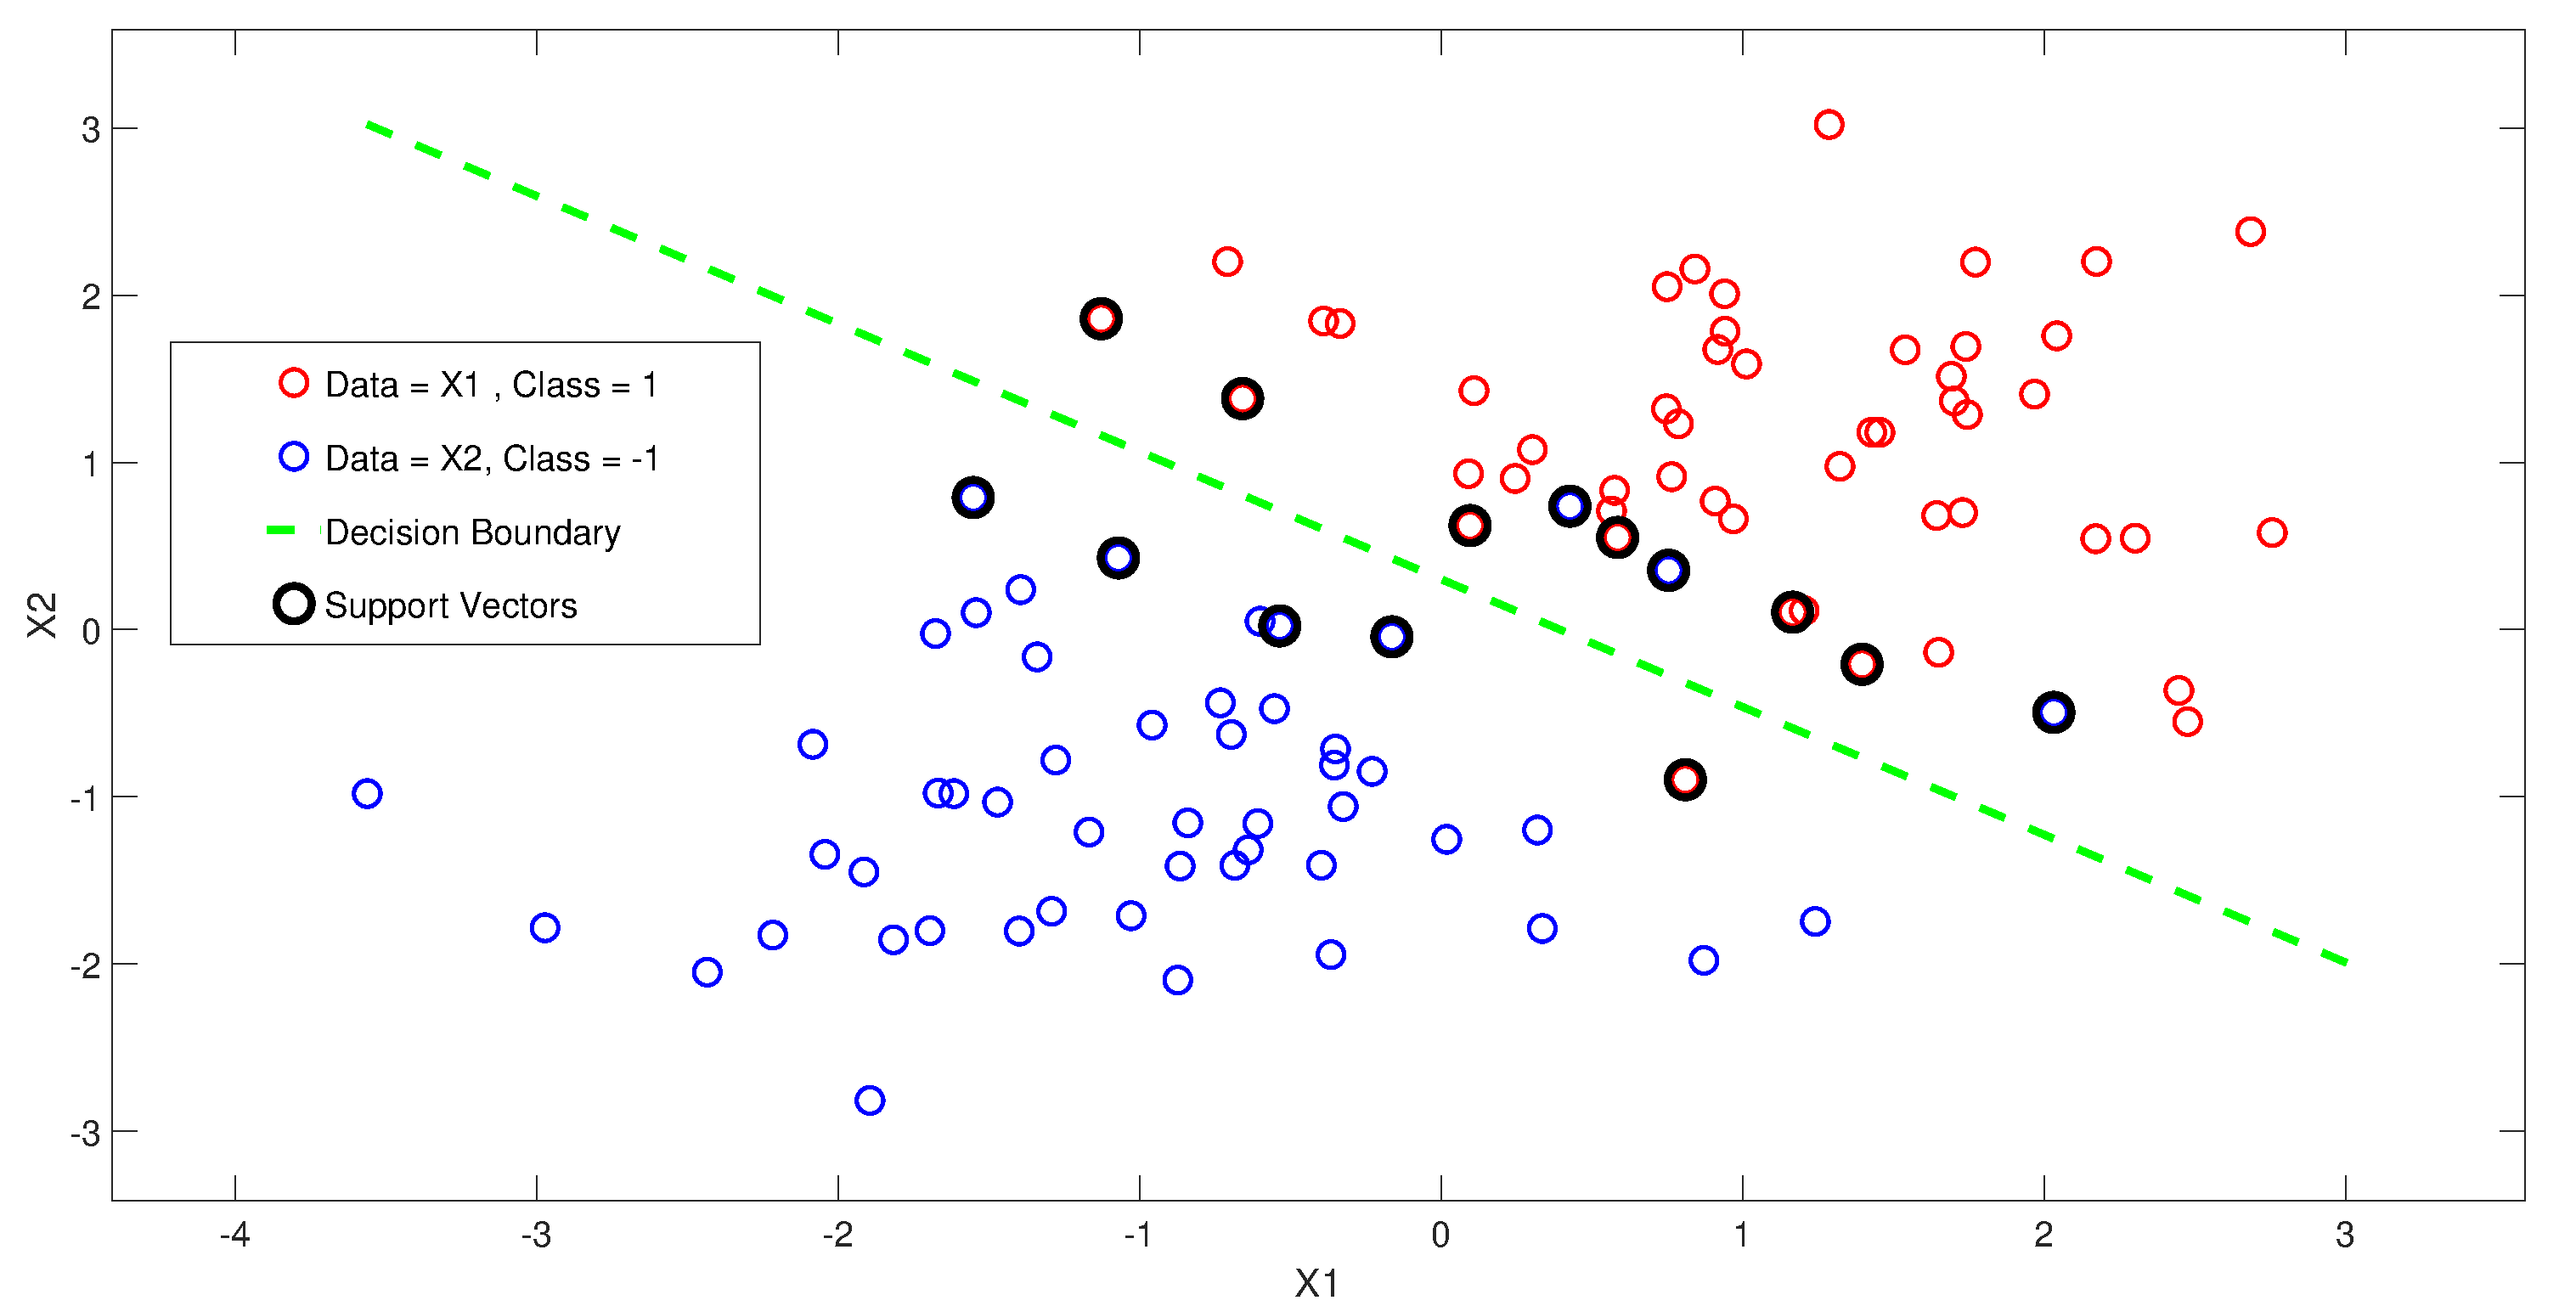
\includegraphics[height=5.5 cm,width= 9 cm]{Exercise1/Report/Ex1.1.eps} 
	 		\caption{Classification}
	 		\label{fig:SVC}
	 	\end{center}
	\end{wrapfigure}
 
	 SVM uses few data points from the training data as support vectors that determines the weights and position of hyper planes. The below equation define the hyper plane of a SVM.
	 \begin{equation}\label{eq:1}
	 \centering
	 f(x)=x{\beta}+b
	 \end{equation}
	  where $\beta$ is the linear predictor coefficient and $b$ is the bias term.  These $\beta$ and $b$ terms are the optimal values of a hyper plane learnt by the classifier as it maximizes the distance between the hyper plane and support vectors. This is done by solving the Lagrange equation using optimization techniques. We train the SVM classifier on our input data set using {\textit{ fitcsvm}} in Matlab. 
	  Hence, the separating line (in our case the green line in the figure \ref{fig:SVC}) that is drawn using the values of $\beta$ and $b$ is an optimal one that allows only few misclassifications as shown in the figure \ref{fig:SVC}.  
	  \subsection{Support Vector Machine Classifier:}	
	  For classes with linearly separable observations, SVM tries to classify the points with a line in such a way that the separation between those classes is maximum.
	  As we know from solving the Lagrangian equation, the solution must satisfy the following the relations
	  \begin{equation}\label{eq:2}
	  \centering
	  w = \sum_{i=1}^{N} \alpha_i y_i x_i , \sum_{i=1}^{N} \alpha_i y_i = 0
	  \end{equation}
	  Solving the above equation \ref{eq:2} using dual problem we get $\alpha_i$.

	   The below figures \ref{fig:lin_rbf1} and \ref{fig:lin_rbf2} shows SVM classifier with linear and RBF kernels. In figure \ref{fig:lin1} and \ref{fig:rbf1} it can be seen that the data points are on the right side of their respective classes. There is not much change in the decision boundary even after adding more points on the same side of the class. Both linear and RBF kernels produce same classification output.
	   

	  \begin{figure}[ht] 
	  	\centering
	  	\begin{subfigure}{.3\textwidth}
	  		\centering
	  		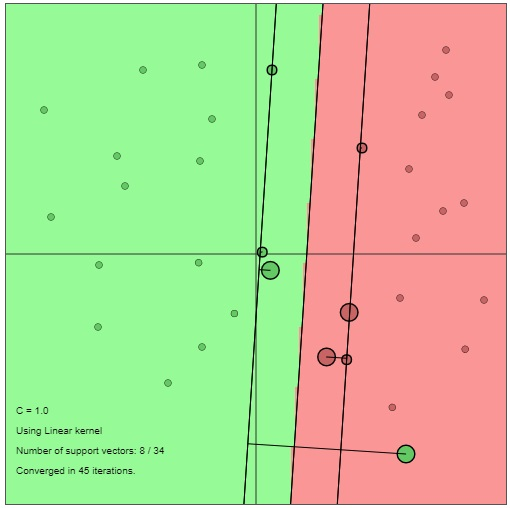
\includegraphics[width=.7\linewidth]{Exercise1/Report/linear_kernel_1.jpg}
	  		\caption{Points on right side}
	  		\label{fig:lin1}
	  	\end{subfigure}%
  		\begin{subfigure}{.3\textwidth}
  			\centering
  			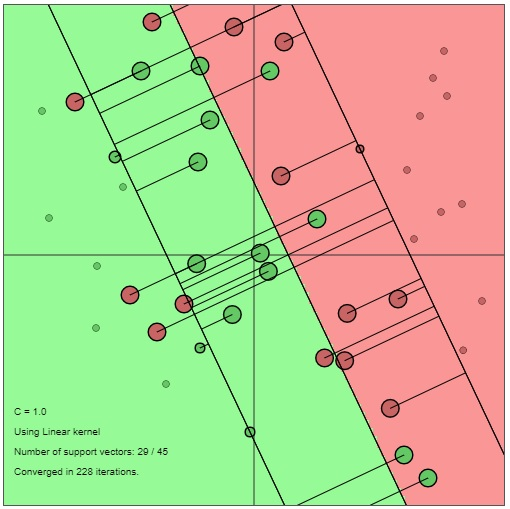
\includegraphics[width=.7\linewidth]{Exercise1/Report/linear_kernel_2.jpg}
  			\caption{Points on wrong side}
  			\label{fig:lin2}
  		\end{subfigure}%
  		\begin{subfigure}{.3\textwidth}
  			\centering
  			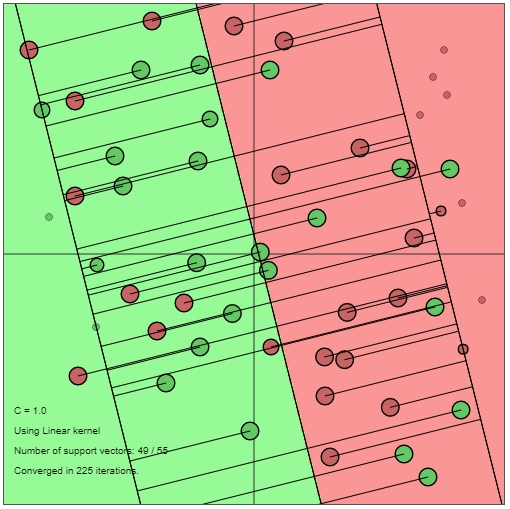
\includegraphics[width=.7\linewidth]{Exercise1/Report/linear_kernel_3.jpg}
  			\caption{More points on wrong side}
  			\label{fig:lin3}
  		\end{subfigure}%
  		\caption{SVM Classification with Linear Kernel}
  		\label{fig:lin_rbf1}
  	  \end{figure}
    
	   In figures \ref{fig:lin2} and \ref{fig:rbf2} few points of one class are added on the wrong sides of hyper plane. In this case, the new points influence the decision boundary and more number of non-zero elements of $\alpha_i$ occur from equation \ref{eq:2}. Also, the soft margin increases as seen in fig \ref{fig:lin2}. Since, the data points are not linearly separable, the SVM classifier with linear kernel takes more number of support vectors (elements with $\alpha_i \neq 0$) into account while deciding a decision boundary.  This accounts for few misclassifications. When it comes to the classifier with RBF kernel in fig \ref{fig:rbf2}, it classifies all the data points correctly with no misclassifications. 

     
	\begin{figure}[ht] 
		\centering
	 	\begin{subfigure}{.3\textwidth}
	 		\centering
	 		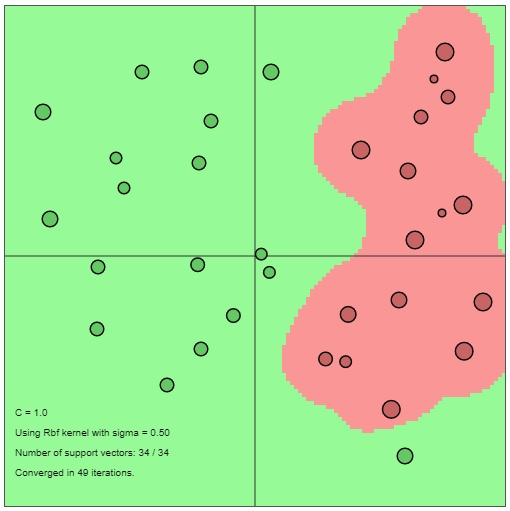
\includegraphics[width=.7\linewidth]{Exercise1/Report/RBF_kernel_1.jpg}
	 		\caption{Points on right side}
	 		\label{fig:rbf1}
	 	\end{subfigure}
		 \begin{subfigure}{.3\textwidth}
	 		\centering
	 		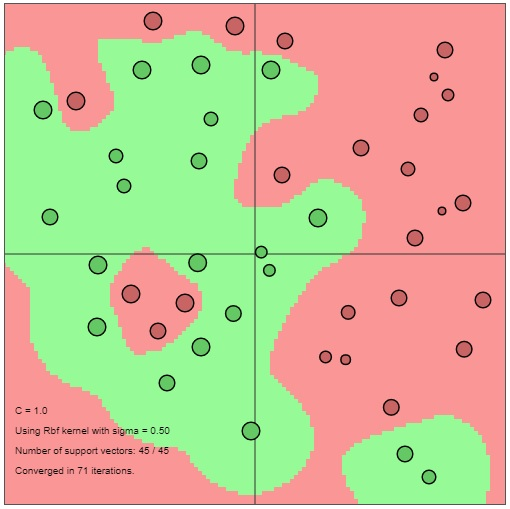
\includegraphics[width=.7\linewidth]{Exercise1/Report/RBF_kernel_2.jpg}
	 		\caption{Points on wrong side}
	 		\label{fig:rbf2}
	 	\end{subfigure}
	 	\begin{subfigure}{.3\textwidth}
 			\centering
 			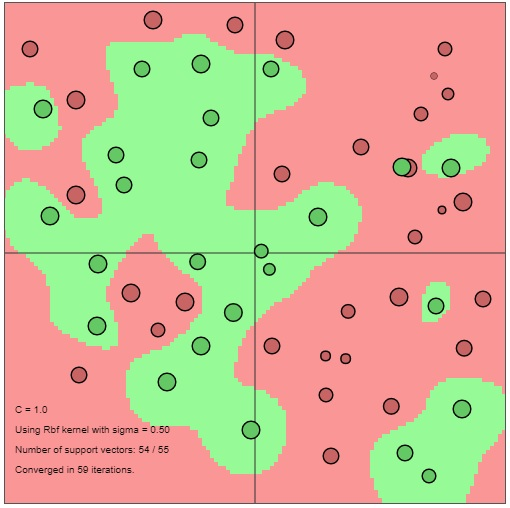
\includegraphics[width=.7\linewidth]{Exercise1/Report/RBF_kernel_3.jpg}
 			\caption{More points on wrong side}
 			\label{fig:rbf3}
 		\end{subfigure}
	 	\caption{SVM Classification with data points on wrong side of a hyperplane}
	 	\label{fig:lin_rbf2}
	\end{figure}
 
    
In figures \ref{fig:lin3} and \ref{fig:rbf3} more points of one class are added on the wrong sides of the hyper plane. Wrong data points affect the decision boundary to a great extent with linear kernel and the soft margin becomes wide in figure \ref{fig:lin3}. It can be observed in figure \ref{fig:lin3} that even though linear kernel takes almost every point as a support vector, it still fails to give a good decision boundary and a lot of misclassifications occur. This means, changing the support vectors can change the decision boundary. But the classifier with RBF kernel, classifies all the data points correctly with only one misclassification as seen in figure \ref{fig:rbf3}. \\\\
\textbf{Try out different values of the regularization hyperparameter C and the kernel parameter sigma. What is the role of the parameters? How do these parameters
affect the classification outcome?}
 
 The parameter C is responsible for optimization. It tells the SVM classifier about how much misclassification it can allow on a given data set. For some larger value of C, the SVM classifier will give us a hyperplane with smaller margin and classify all the training data points correctly. Conversely for some smaller value of C, the SVM will give us a hyperplane with wider margin and allows some misclassifications even if the training data is linearly separable.

Sigma determines the reach of a training data point. For a smaller value of sigma, the SVM classifier reaches to the training points that are further away from the margin. This can lead to over-fitting of the model. For larger values of sigma, the model looks for points that are closer and it will be able to generalize better. The effect of these hyper parameters C and sigma is explained in detail in the below question.\\\\
\textbf{Compare classification using the linear kernel with classification using the RBF kernel. Which performs better? Why?}
 	 
 	 As seen from figures \ref{fig:lin1} and \ref{fig:rbf1}, the classifier with RBF and linear kernels gives similar performance as the data points are linearly separable. But from figures \ref{fig:lin2}, \ref{fig:rbf2}, \ref{fig:lin3} and \ref{fig:rbf3} we can observe that the data is non-linearly separable and RBF out performs the classifier with linear kernel. What RBF does is, it creates a non-linear combination of the data features and project them onto a higher-dimensional space. It later separates the classes with a linear decision boundary(kernel trick) . Training the SVM classifier with linear kernel takes lesser time when compared to RBF kernel. Therefore, linear kernel can do the job for linearly separable data points. But, for non-linearly separable data RBF would be a better choice \\\\
\textbf{ What is a support vector? When does a particular datapoint become a support vector? When does the importance of the support vector change? Illustrate visually.}
	
\begin{wrapfigure}{r}{.4\textwidth}
	\begin{minipage}{\linewidth}
		\centering\captionsetup[subfigure]{justification=centering}
		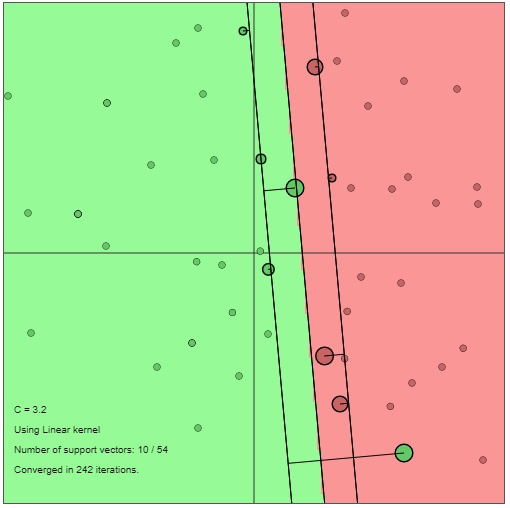
\includegraphics[height=0.6\linewidth, width=0.65\linewidth]{Exercise1/Report/lin_SV1.jpg}
		\subcaption{Linearly Separable Points}
		\label{fig:SV1}\par\vfill
		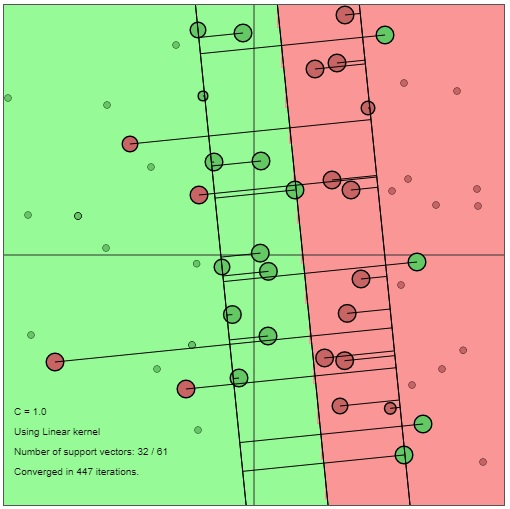
\includegraphics[height=0.6\linewidth, width=0.65\linewidth]{Exercise1/Report/lin_SV2.jpg}
		\subcaption{Non-linearly Separable Points}
		\label{fig:SV2}
	\end{minipage}
	\caption{Support Vectors during classification}
	\label{fig:SV}
\end{wrapfigure}
Support vectors are nothing but the training data points which lie on(or inside of) the margin line. SVM tries to find an optimal hyper plane $y(x) = w^Tx_i+b$ such that for an unknown value of $x$, it gives the class of $x$. Therefore, its goal is to estimate $w$. As given in equation \ref{eq:2} when we solve the Lagrangian dual of SVM, we get $w = \sum_{i=1}^{N} \alpha_i y_i x_i $. 
	Substituting the value of $w$ in $y(x)$ gives the below equation.
	 \begin{equation}\label{eq:3}
	\centering
	y(x)=\sum_{i=1}^{N} \alpha_i y_i x_i^T x+b
	\end{equation}
	Here $\alpha_i$ are the variables of duality. A data point becomes a support vector when the $\alpha_i$ value is non-zero and the point lie on or inside the margin line. Equation \ref{eq:3} denotes the sparse representation of SVM.
	It can be seen from eq \ref{eq:3} that our linear classifier is represented using only the points that lie on or inside the margin line. With this we can now  transform the  SVM into a non-linear classifier using the kernel trick and compute classification hyperplanes in large dimensional spaces as y(x) is now only a dot product of terms.  From figure \ref{fig:SV}, it can be seen that in the case of linearly separable points (fig \ref{fig:SV1}), the support vectors are fewer in number and the soft margin has a smaller width. The one misclassified green point is also considered as a support vector. Whereas, in the case of non-linearly separable points (fig \ref{fig:SV2}) every misclassified point is considered as a support vector and SVM takes lot more points in arriving at a decision boundary. Also, the width of the soft margin is huge in figure \ref{fig:SV1} compared to the one in figure \ref{fig:SV1}. Hence, we can say that the support vectors are responsible for the position and orientation of a hyper plane.\\\\
\textbf{What is the role of parameters C and sigma? What happens to the classification boundary if you change these parameters. Illustrate visually.}\\
The regularization parameter C controls the misclassifications done by SVM classifier. The effect of C is illustrated in the following figures.


\begin{figure}[!ht] 
	\centering
	\begin{subfigure}{.32\textwidth}
		\centering
		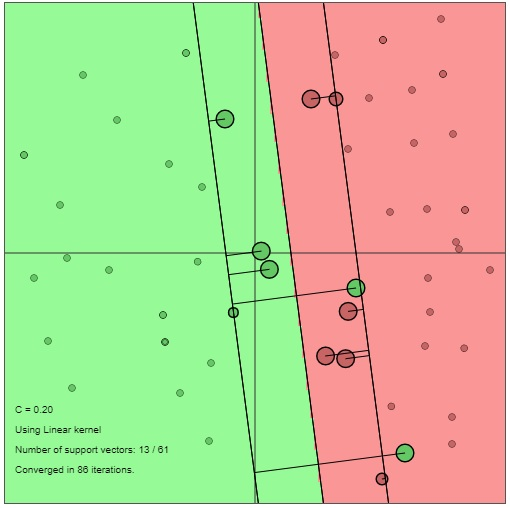
\includegraphics[width=.65\linewidth]{Exercise1/Report/lin_C(0.2).jpg}
		\caption{C = 0.2}
		\label{fig:C0.2}
	\end{subfigure}%
	\begin{subfigure}{.32\textwidth}
		\centering
		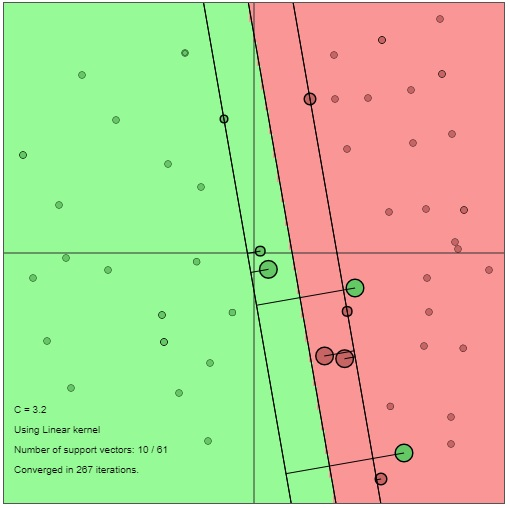
\includegraphics[width=.65\linewidth]{Exercise1/Report/lin_C(3.2).jpg}
		\caption{C = 3.2}
		\label{fig:C3.2}
	\end{subfigure}
	\begin{subfigure}{.32\textwidth}
		\centering
		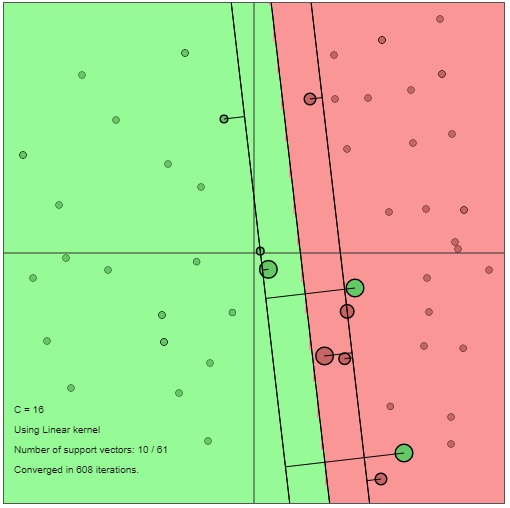
\includegraphics[width=.65\linewidth]{Exercise1/Report/lin_C(16).jpg}
		\caption{C = 16}
		\label{fig:C16}
	\end{subfigure}
	\caption{SVM with Linear Kernel and change in C values}
	\label{fig:C}
\end{figure}

\begin{figure}[!ht] 
	\centering
	\begin{subfigure}{.32\textwidth}
		\centering
		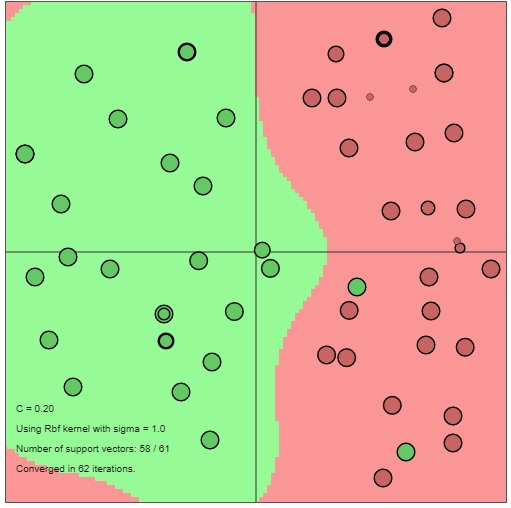
\includegraphics[width=.65\linewidth]{Exercise1/Report/RBF_C(0.2).jpg}
		\caption{C = 0.2}
		\label{fig:RBF0.2}
	\end{subfigure}%
	\begin{subfigure}{.32\textwidth}
		\centering
		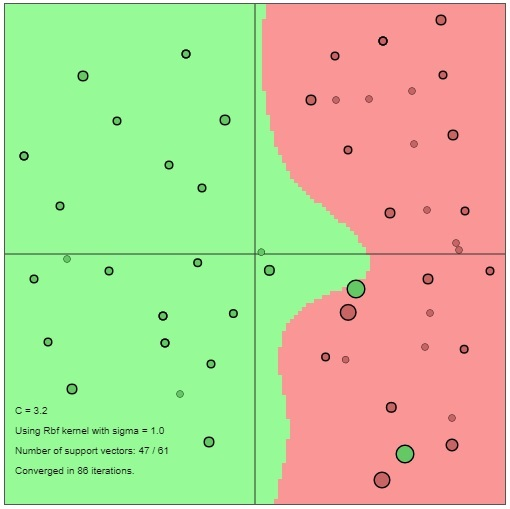
\includegraphics[width=.65\linewidth]{Exercise1/Report/RBF_C(3.2).jpg}
		\caption{C = 3.2}
		\label{fig:RBF3.2}
	\end{subfigure}
	\begin{subfigure}{.32\textwidth}
		\centering
		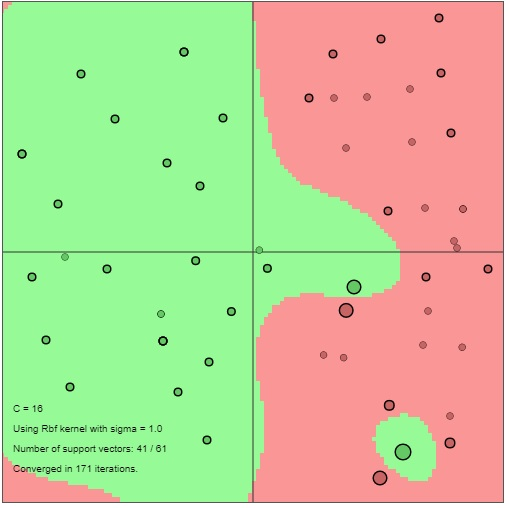
\includegraphics[width=.65\linewidth]{Exercise1/Report/RBF_C(16).jpg}
		\caption{C = 16}
		\label{fig:RBF16}
	\end{subfigure}
	\caption{SVM with RBF Kernel and change in C values}
	\label{fig:RBF}
\end{figure}

From figure \ref{fig:C16}, it can be seen that for a value of C=16, the decision boundary for a linear kernel has smaller margin and has less number of support vectors. For the same value of C in figure \ref{fig:RBF16}, the RBF kernel correctly classifies all the training points.
As the C value is reduced to 0.2 and 3.2 in figures \ref{fig:C0.2} and \ref{fig:C3.2}, the linear kernel uses more support vectors and also accounts to misclassifications. The soft margin becomes wider for lesser values of C. Similarly for the RBF kernel in figures \ref{fig:RBF0.2} and \ref{fig:RBF3.2}, misclassifications occur for smaller value of C. Therefore, from figures \ref{fig:C} and \ref{fig:RBF}, it can be said that the a larger value of C makes the model over-fit while a smaller value makes it under fit. 

The RBF kernel for SVM classifier in dual space is given as below
\begin{equation}\label{eq:4}
	k(x,x_i)= exp{\Bigg(-\dfrac{||x-x_i||^2_2}{\sigma^2} \Bigg)}
\end{equation}
From the above equation \ref{eq:4}, it can be seen that the value of $\sigma$ influences the distance between $x$ and $x_i$. The value of $k(x,x_i)$ tends to zero when $\sigma$ is much smaller than $||x-x_i||^2_2$. This can make the classifier reach points that are further away which leads to over fitting. As the value of $\sigma$ increases, the classifier will look for points that are closer and hence it will generalize better.\\
\begin{figure}[!ht] 
	\centering
	\begin{subfigure}{.255\textwidth}
		\centering
		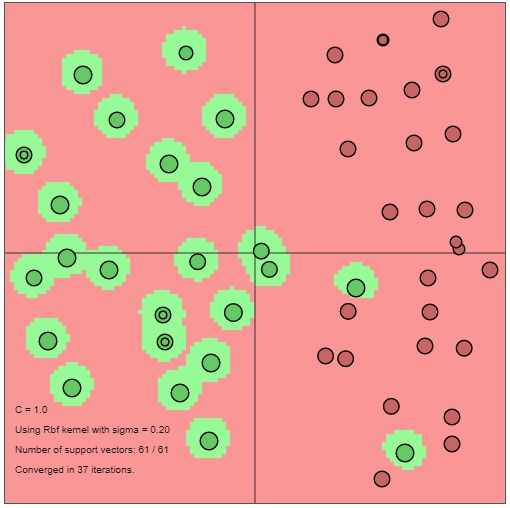
\includegraphics[width=0.8\linewidth]{Exercise1/Report/RBF_sigma(0.2).jpg}
		\caption{Sigma = 0.2}
		\label{fig:RBF_sig0.2}
	\end{subfigure}%
	\begin{subfigure}{.255\textwidth}
		\centering
		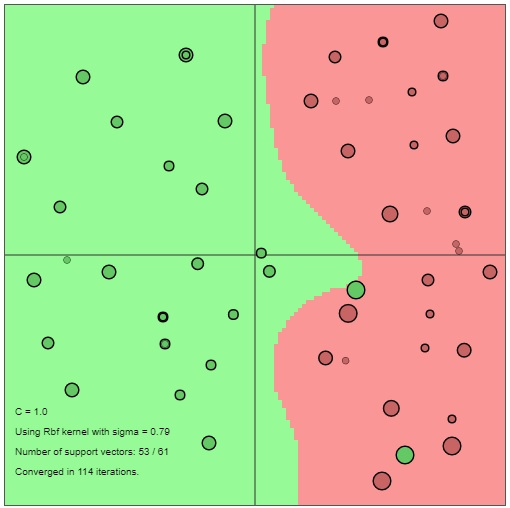
\includegraphics[width=0.8\linewidth]{Exercise1/Report/RBF_sigma(0.79).jpg}
		\caption{Sigma = 0.79}
		\label{fig:RBF_sig0.79}
	\end{subfigure}%
	\begin{subfigure}{.255\textwidth}
		\centering
		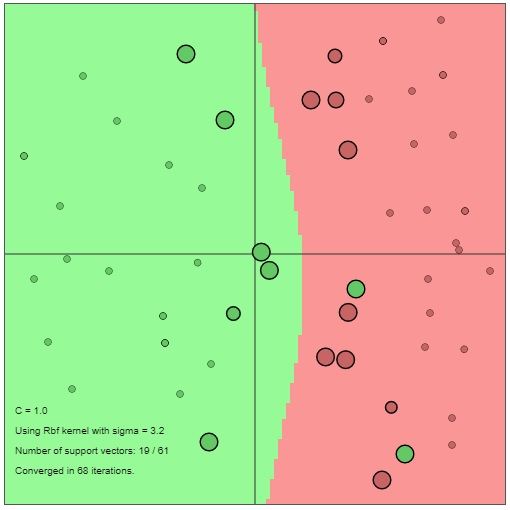
\includegraphics[width=0.8\linewidth]{Exercise1/Report/RBF_sigma(3.2).jpg}
		\caption{Sigma = 3.2}
		\label{fig:RBF_sig3.2}
	\end{subfigure}%
	\begin{subfigure}{.255\textwidth}
		\centering
		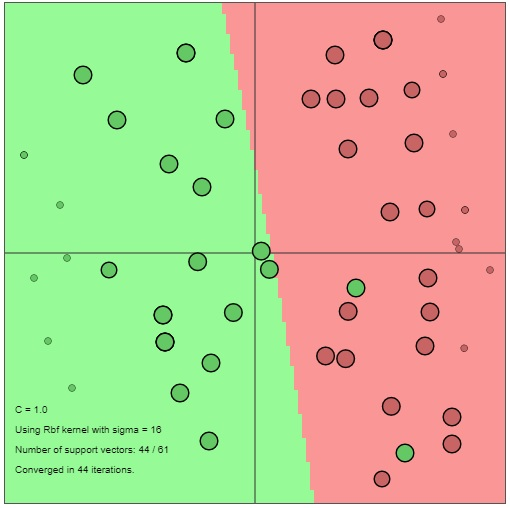
\includegraphics[width=0.8\linewidth]{Exercise1/Report/RBF_sigma(16).jpg}
		\caption{Sigma = 16}
		\label{fig:RBF_sig16}
	\end{subfigure}%
	\caption{SVM with RBF Kernel and change in sigma values}
	\label{fig:RBF_sig}
\end{figure}
In figure \ref{fig:RBF_sig}, it can be seen that for a smaller value of $\sigma = 0.2$
the classifier tries to fit all the data points which indicates over fitting. As the value of $\sigma$ increases to 0.79, 0.32 and 16, the model generalizes better. \\\\
\textbf{What happens to the classification boundary when sigma is taken very large? Why?}

As seen from figure \ref{fig:RBF_sig16}, for a higher value of $\sigma = 16$ the model generalizes better and gives almost a linear decision boundary. This means that the area of impact of support vectors will include only the support vectors.

\subsection{Least-Squares Support Vector Machine Classifier:}
\subsubsection{Influence of hyperparameters and kernel parameters }
\textbf{Try out a polynomial kernel with degree = 1; 2; 3; ... and t = 1 (fix gam = 1). Assess	the performance on the test set. What happens when you change the degree of the polynomial kernel?}

\begin{wraptable}{l}{8.5cm}
	\caption{Error rate of polynomial kernel on test set}\label{table:1}
	\begin{tabular}{|c|c|c|}
		\hline
		Degree & Misclassifications & Error Rate \\
		&&on test set (\%)\\ \hline
		1 &11 & 55.00 \\ \hline
		3 &0 & 0 \\  \hline
		5 &0 & 0 \\  \hline
		7 &0 & 0 \\  \hline
		9 &0 & 0 \\  \hline
		11 &0 & 0 \\ \hline
	\end{tabular}
\end{wraptable}
 From the figure \ref{fig:deg} and table \ref{table:1}, it can be observed that for degree = 1, the decision boundary is a linear one and a lot of misclassifications occur on the training data points. Even on test set the classifier gives 11 misclassifications with an error rate of 55 \%. As the degree value is increased, the model performs better and the number of misclassifications are reduced. The classifier gives exact predictions on the test sets for degree values greater than 1. Also, for the polynomial kernels with degree 9 and 11, the model tries to cover all the training samples with complex decision boundaries which indicates that it is moving towards over-fitting. Therefore, a good range of degree values can be between 3 and 9.\\
 \begin{figure}[!htbp] 
 	\centering
 	\begin{subfigure}{.33\textwidth}
 		\centering
 		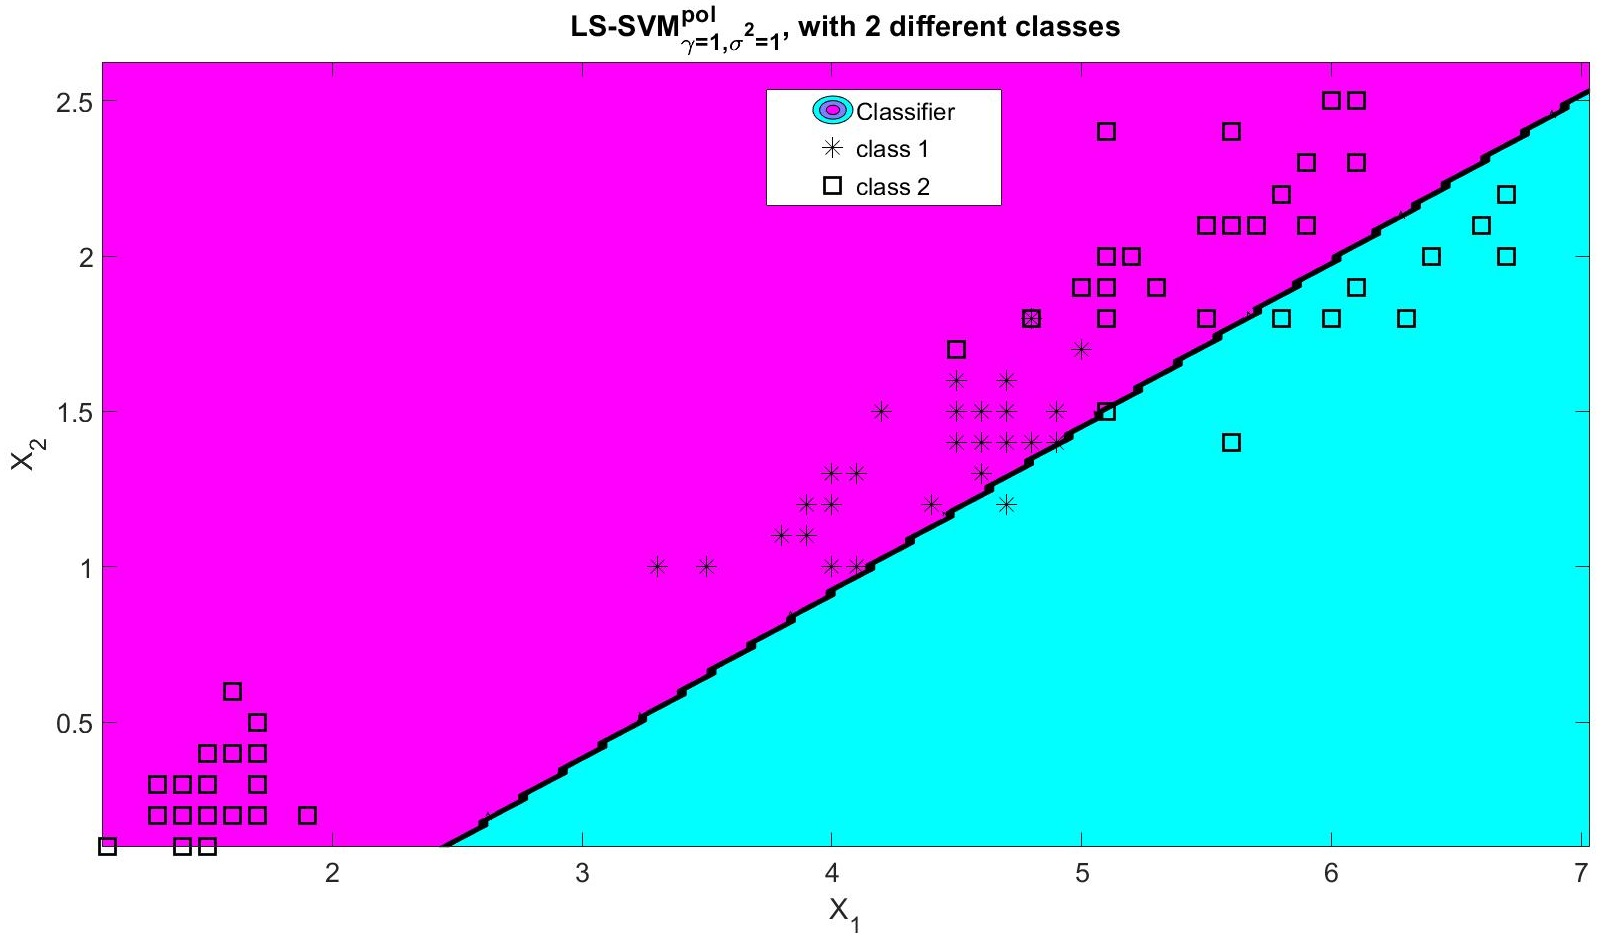
\includegraphics[height=0.8\linewidth,width=1\linewidth]{Exercise1/Report/Ex1.3_deg(1).jpg}
 		\caption{Degree = 1}
 		\label{fig:deg(1)}
 	\end{subfigure}%
 	\begin{subfigure}{.33\textwidth}
 		\centering
 		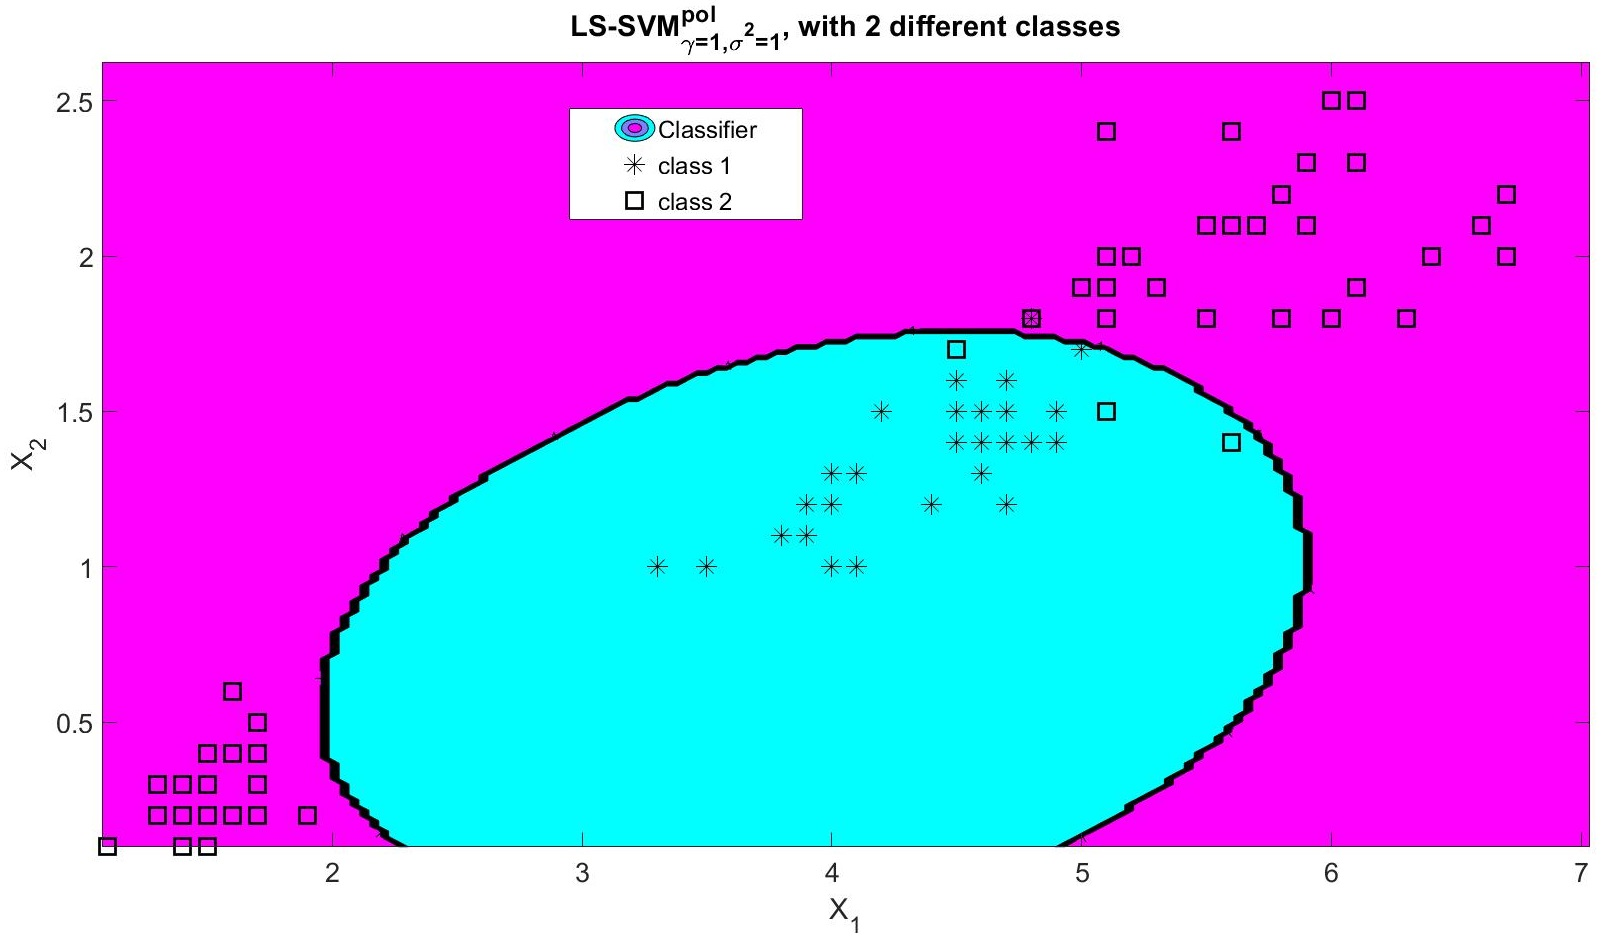
\includegraphics[height=0.8\linewidth,width=1\linewidth]{Exercise1/Report/Ex1.3_deg(3).jpg}
 		\caption{Degree = 3}
 		\label{fig:deg31)}
 	\end{subfigure}%
 	\begin{subfigure}{.33\textwidth}
 		\centering
 		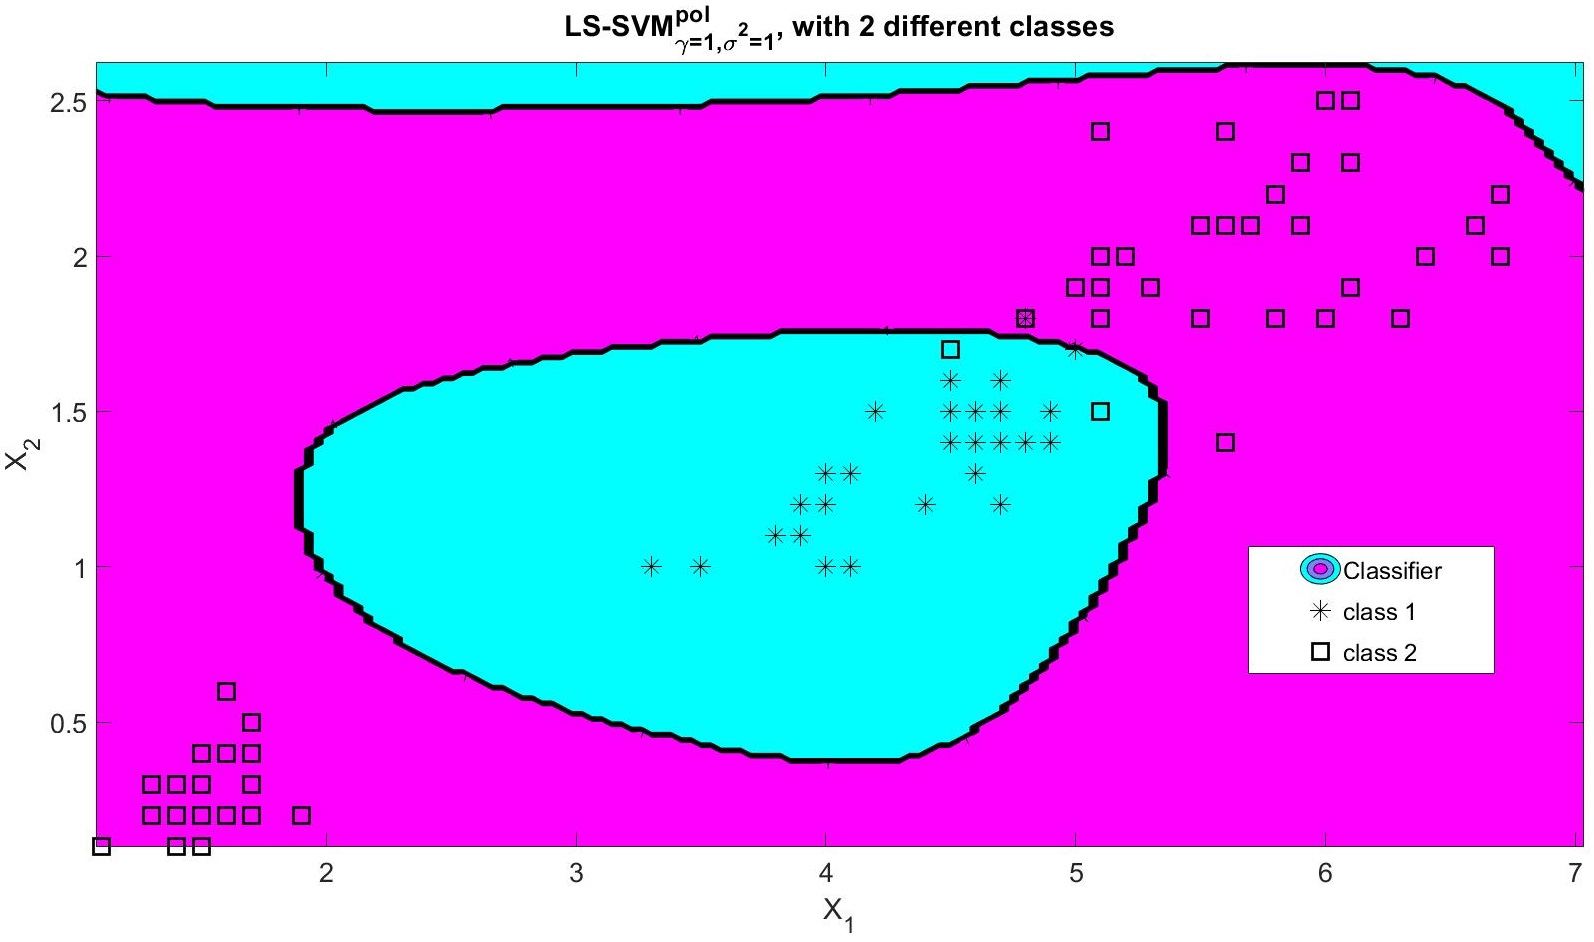
\includegraphics[height=0.8\linewidth,width=1\linewidth]{Exercise1/Report/Ex1.3_deg(5).jpg}
 		\caption{Degree = 5}
 		\label{fig:deg(5)}
 	\end{subfigure}
 	\begin{subfigure}{.33\textwidth}
 		\centering
 		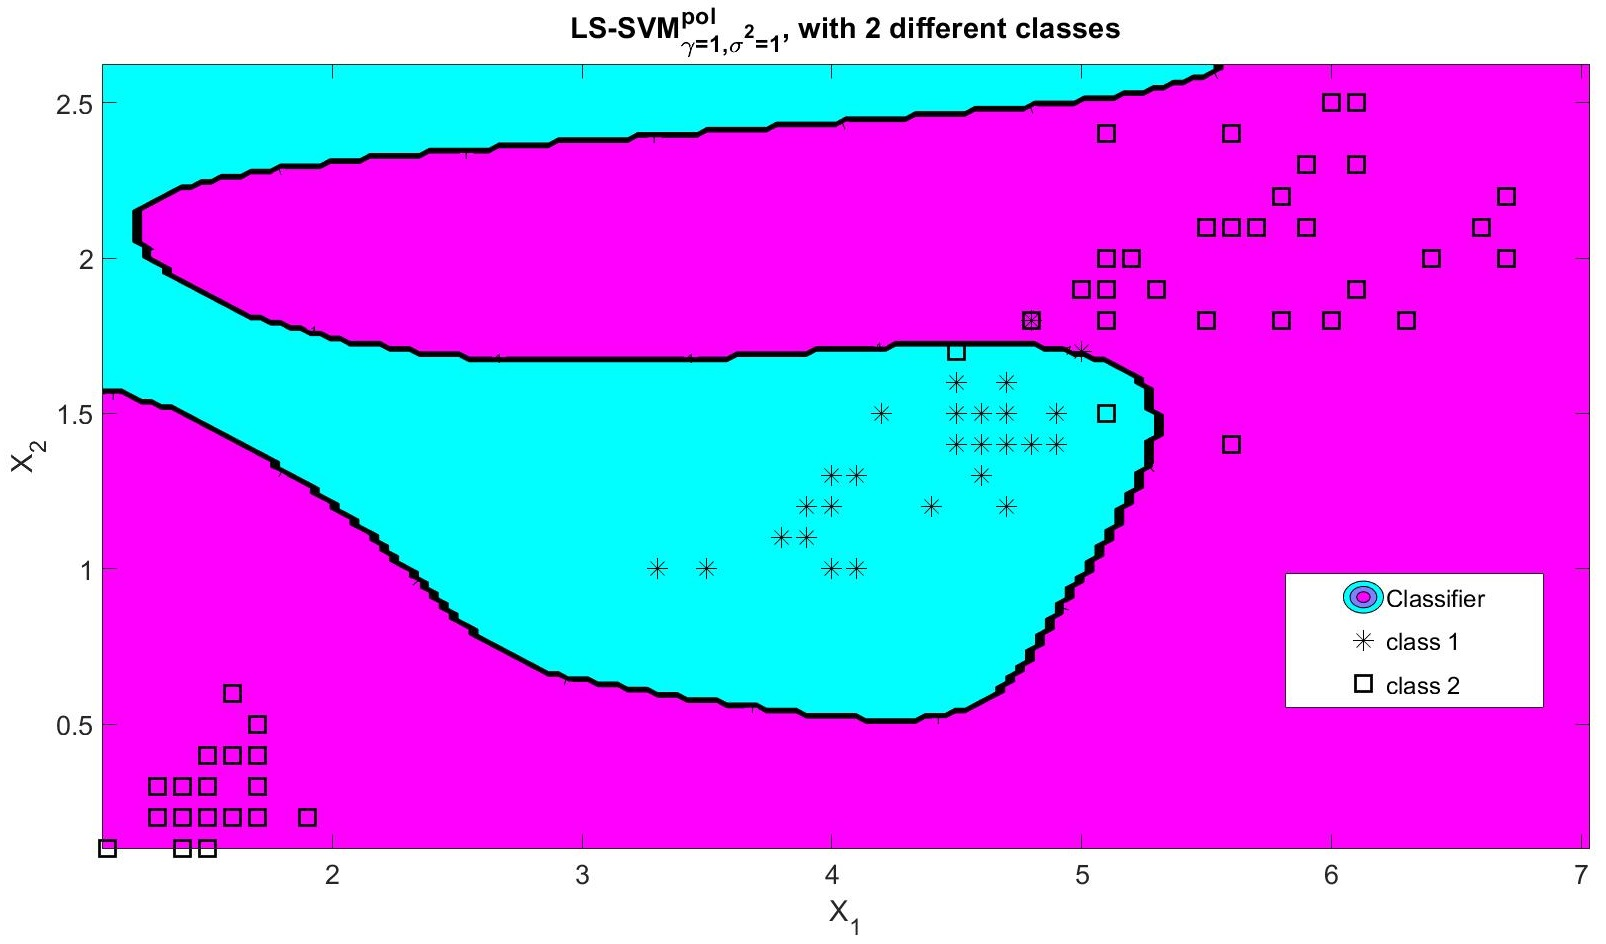
\includegraphics[height=0.8\linewidth,width=1\linewidth]{Exercise1/Report/Ex1.3_deg(7).jpg}
 		\caption{Degree = 7}
 		\label{fig:deg(7)}
 	\end{subfigure}%
 	\begin{subfigure}{.33\textwidth}
 		\centering
 		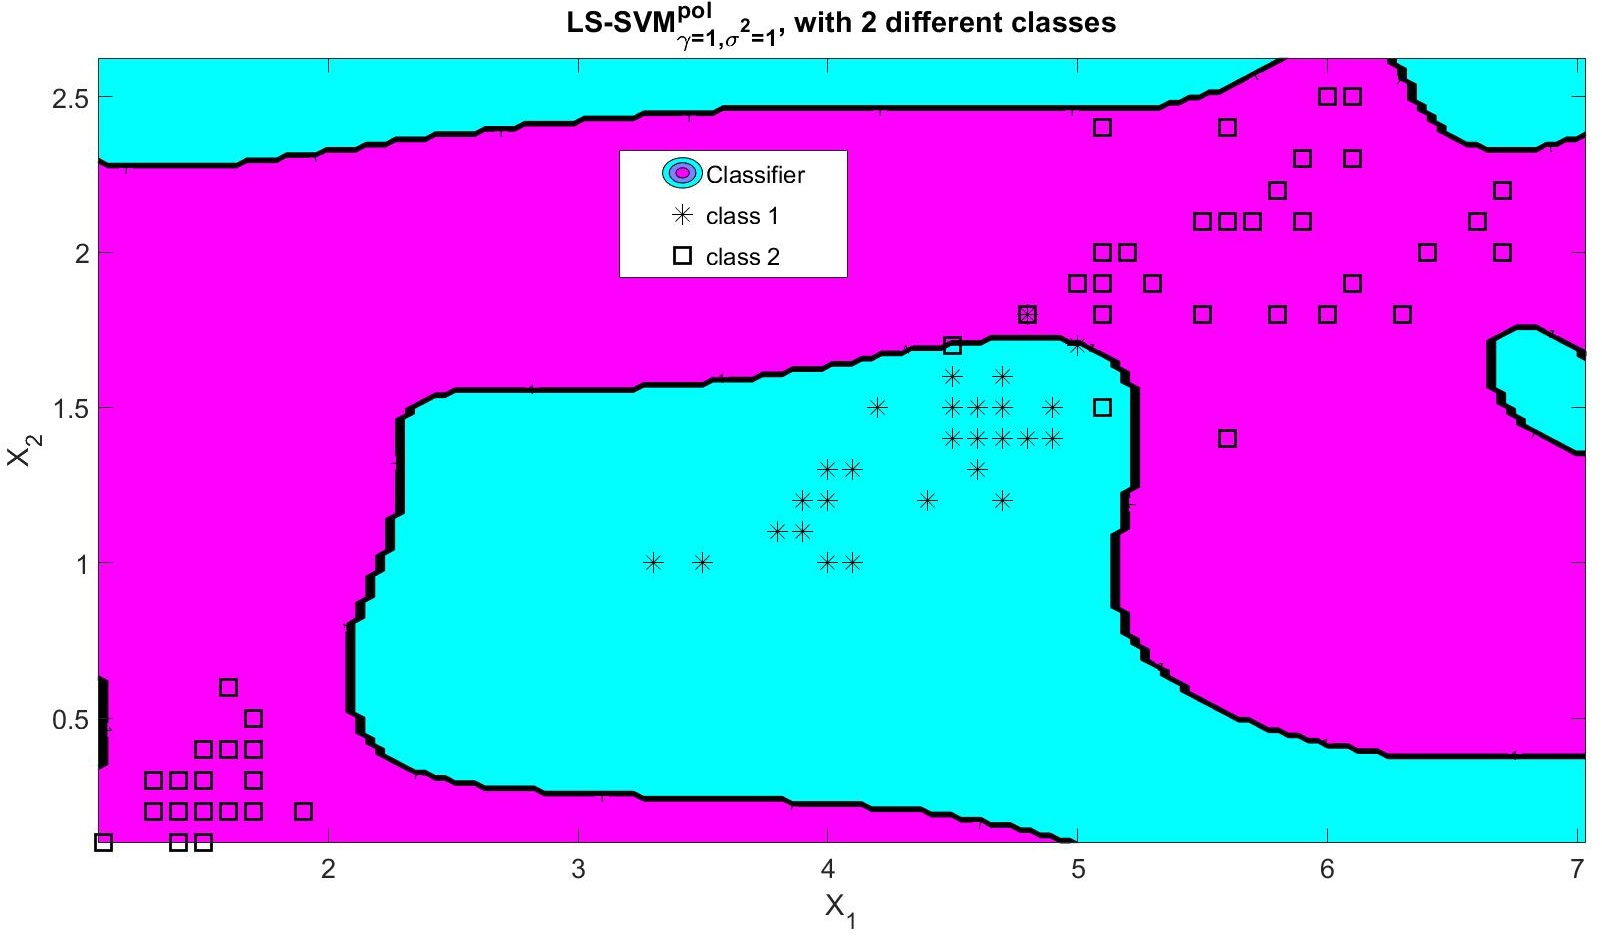
\includegraphics[height=0.8\linewidth,width=1\linewidth]{Exercise1/Report/Ex1.3_deg(9).jpg}
 		\caption{Degree = 9}
 		\label{fig:deg(9)}
 	\end{subfigure}%
 	\begin{subfigure}{.33\textwidth}
 		\centering
 		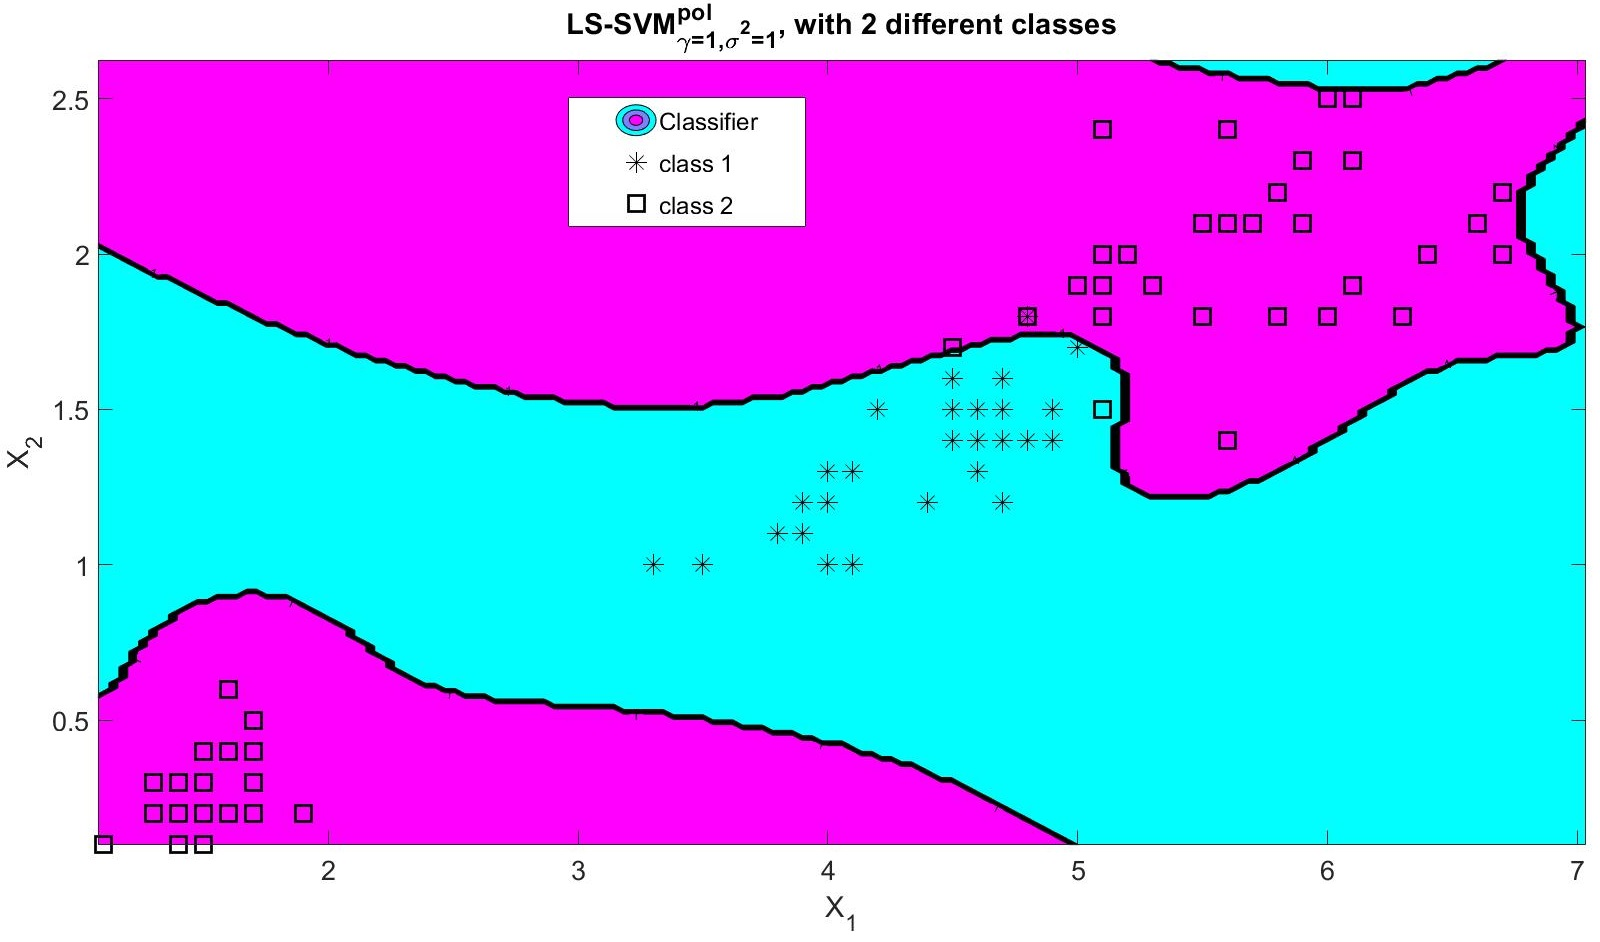
\includegraphics[height=0.8\linewidth,width=1\linewidth]{Exercise1/Report/Ex1.3_deg(11).jpg}
 		\caption{Degree = 11}
 		\label{fig:deg(11)}
 	\end{subfigure}%
 	\caption{SVM with polynomial Kernel and change in degree values}
 	\label{fig:deg}
 \end{figure}\\
 \textbf{Try out a good range of different sig2 values as kernel parameters (fix gam = 1). Assess the performance on the test set. What is a good range for sigma. Fix a reasonable choice for the sig2 parameter and compare the performance using a range of gam. What is a good range for gam?}

As seen from the figure \ref{fig:log_sig} and table \ref{table:2}, the classifier works good on the test set for a range of $\sigma^2$ between 0.1 and 10 when the value of $\gamma$ is fixed to 1. If $\sigma^2$ is increased further, the model performance decreases and gives lot of misclassifications.
\begin{figure}[!ht]
	\begin{floatrow}
		\ffigbox{%
			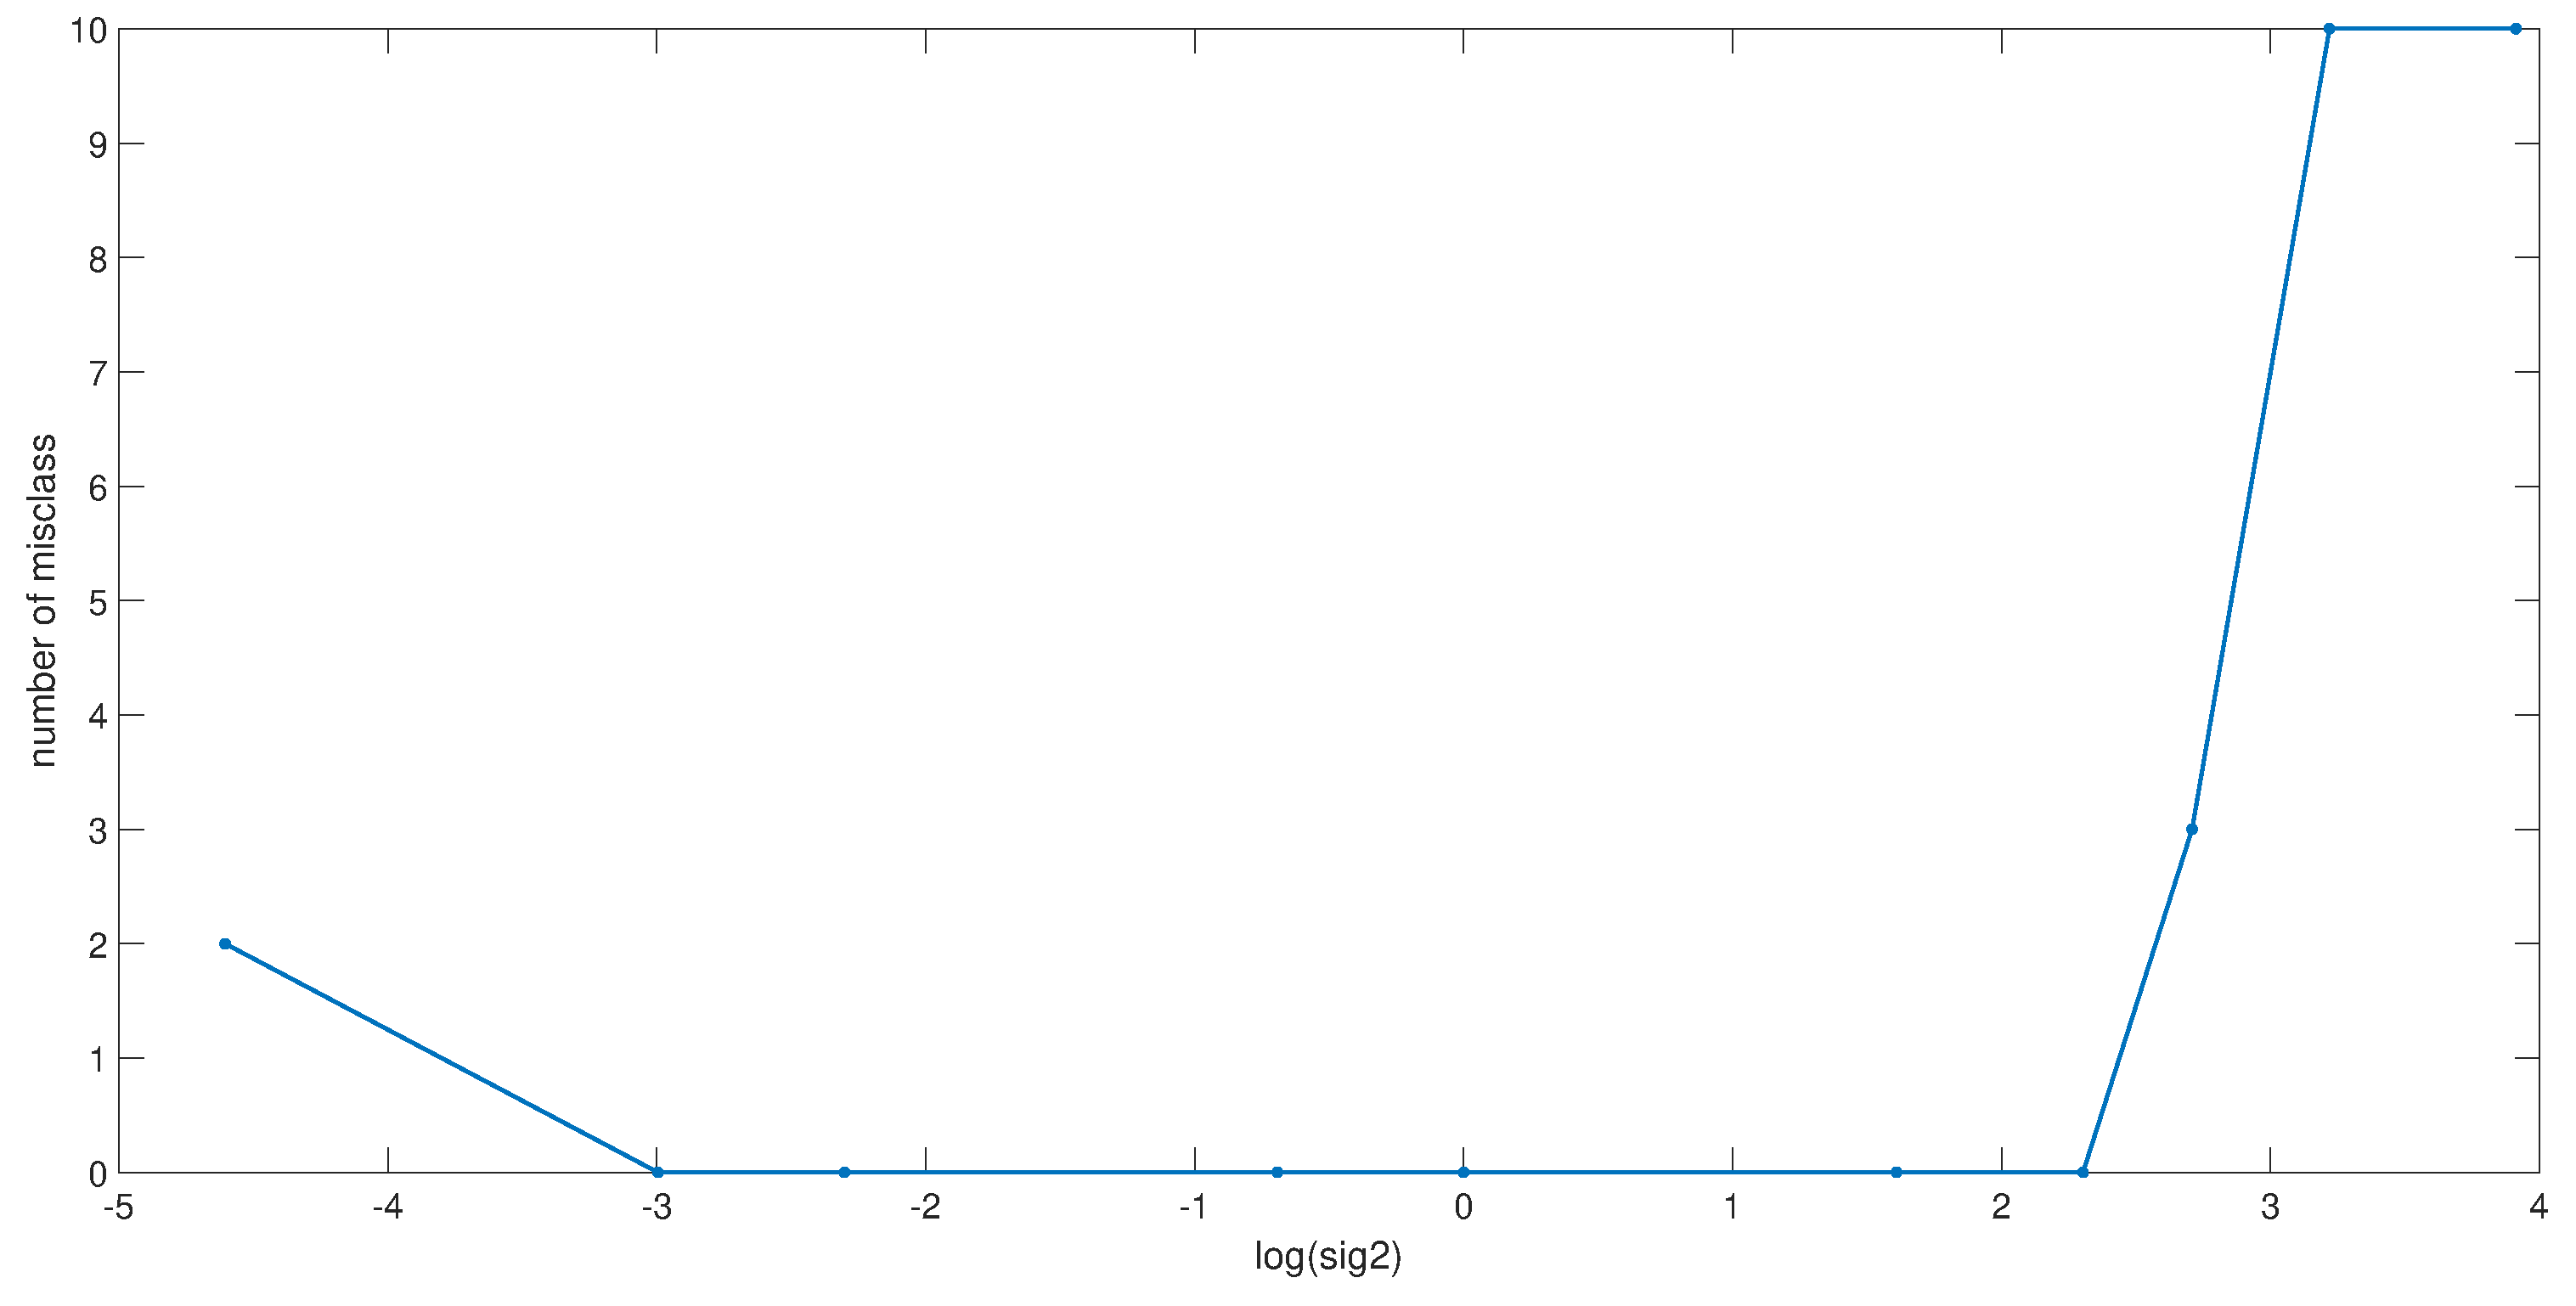
\includegraphics[height=5cm,width=5.5cm]{Exercise1/Report/no_clssVS_sig.eps}%
		}{%
			\caption{log($\sigma^2$) VS misclassifications}\label{fig:log_sig}%
		}
		\capbtabbox{%
		\begin{tabular}{ | c | c | c | c | }
			\hline
			Gamma & Sigma & Mis- & Error Rate \\
			&& classifications& on test \\
			&&& set (\%)\\ \hline
			1 & 0.01 & 2 & 10	\\ \hline
			1 & 0.05 & 0 & 0	\\ \hline
			1 & 0.1 & 0 & 0 \\ \hline
			1 & 0.5 & 0 & 0 \\ \hline
			1 & 1 & 0 & 0  \\ \hline
			1 & 5 & 0 & 0 \\ \hline
			1 & 10 & 0 & 0 \\ \hline
			1 & 15 & 3 & 15 \\ \hline
			1 & 25 & 10 & 50 \\ \hline
			1 & 50 & 10 & 50 \\ \hline
		\end{tabular}
		
		}{%
		\caption{Performance of SVM for various $\sigma^2$ values}\label{table:2}
		}
	\end{floatrow}
\end{figure}
 
SVM classifier is sensitive to changes in $\gamma$. As, seen from figure \ref{fig:log_gam} and table \ref{table:3}, the model performs poorly for lower values of $\gamma$ and gives stable results for higher values. This means that for $\gamma$ with very small values, the classifier fails to capture the complexity of the data. For $\gamma$ with bigger values, even though the model learns complex shapes, it focuses on smoothing the curve rather than minimizing the errors. This could result in poor performance of model without proper fitting of data points. A good range of $\gamma$ can be between 1 to 5, when $\sigma$ is fixed to 2.
 \begin{figure}[!ht]
 	\begin{floatrow}
 		\ffigbox{%
 			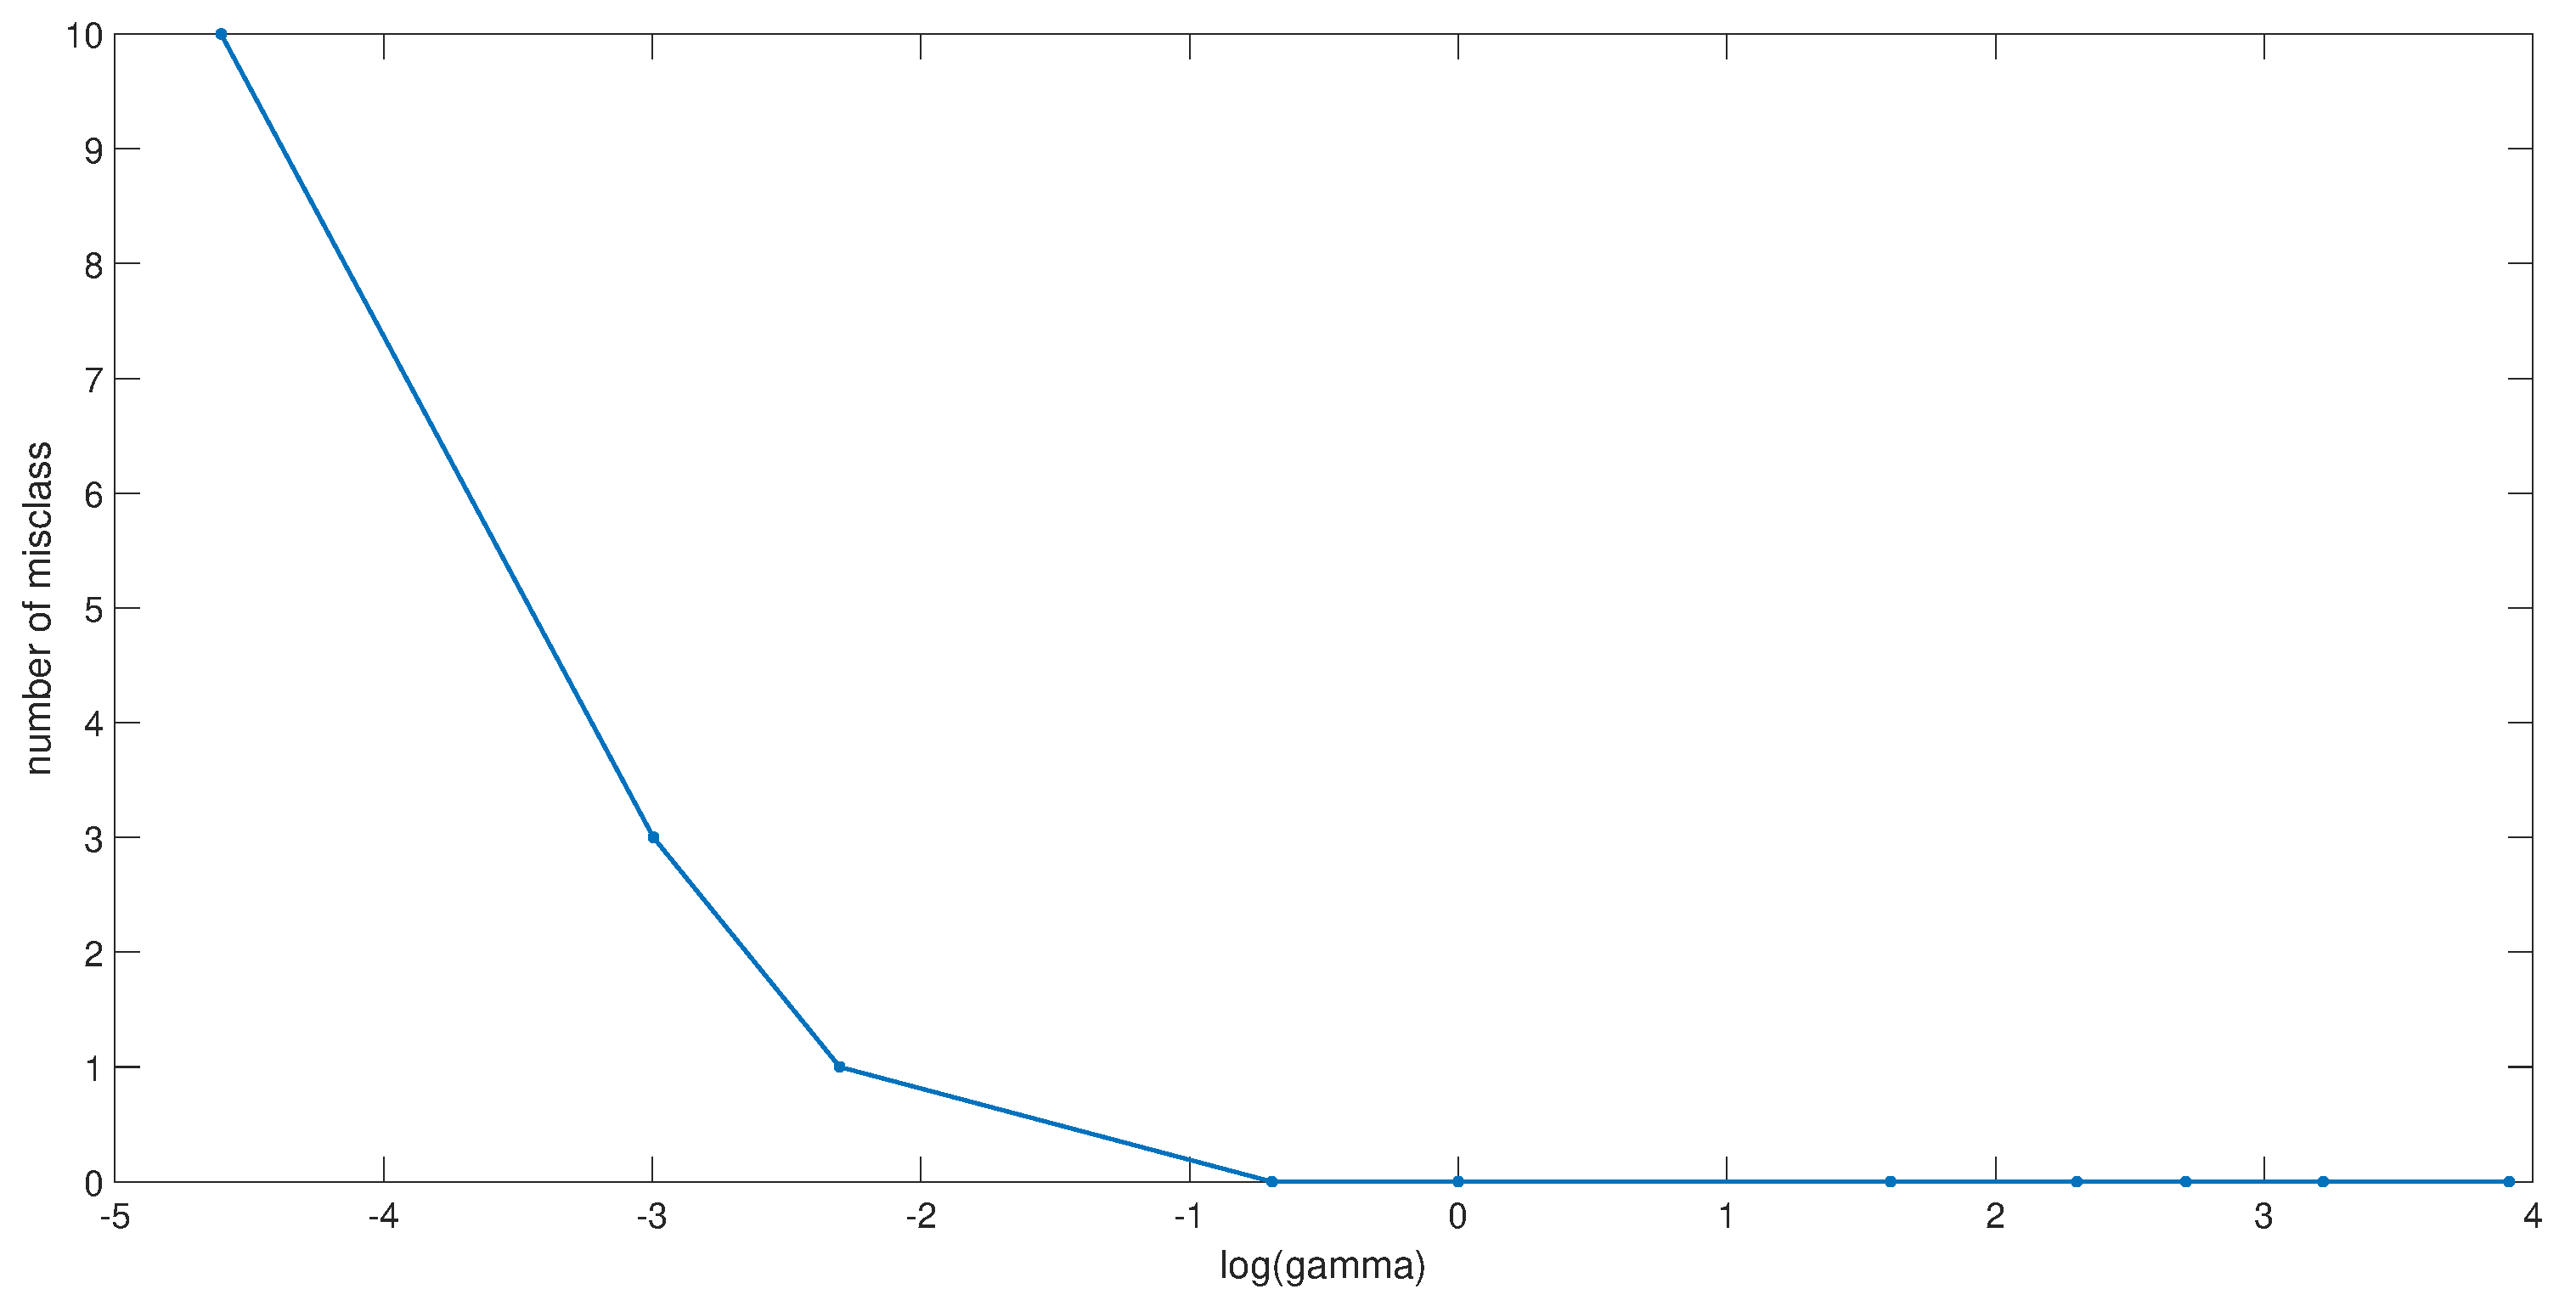
\includegraphics[height=5cm,width=6.7cm]{Exercise1/Report/no_clssVS_gamma.eps}%
 		}{%
 			\caption{log($\gamma$) VS misclassifications}\label{fig:log_gam}%
 		}
 		\capbtabbox{%
 			\begin{tabular}{ | c | c | c | c | }
 				\hline
 				Sigma & Gamma & Mis- & Error Rate \\
 				&& classifications& on test \\
 				&&& set (\%)\\ \hline
 				2 & 0.01 & 10 & 50	\\ \hline
 				2 & 0.05 & 10 & 50 \\ \hline
 				2 & 0.1 & 3 & 15 \\ \hline
 				2 & 0.5 & 1 & 5 \\ \hline
 				2 & 1 & 0 & 0  \\ \hline
 				2 & 5 & 0 & 0 \\ \hline
 				2 & 10 & 0 & 0 \\ \hline
 				2 & 15 & 0 & 0 \\ \hline
 				2 & 25 & 0 & 0 \\ \hline
 				2 & 50 & 0 & 0 \\ \hline
 			
 		\end{tabular}
 			
 		}{%
 			\caption{Performance of SVM for various $\gamma$ values}\label{table:3}
 		}
 	\end{floatrow}
 \end{figure}

Similar results as described above is seen with the script SampleScript\_Iris.m

\subsubsection{Tuning parameters using validation}
 \begin{figure}[!ht]
	\begin{floatrow}
		\ffigbox{%
			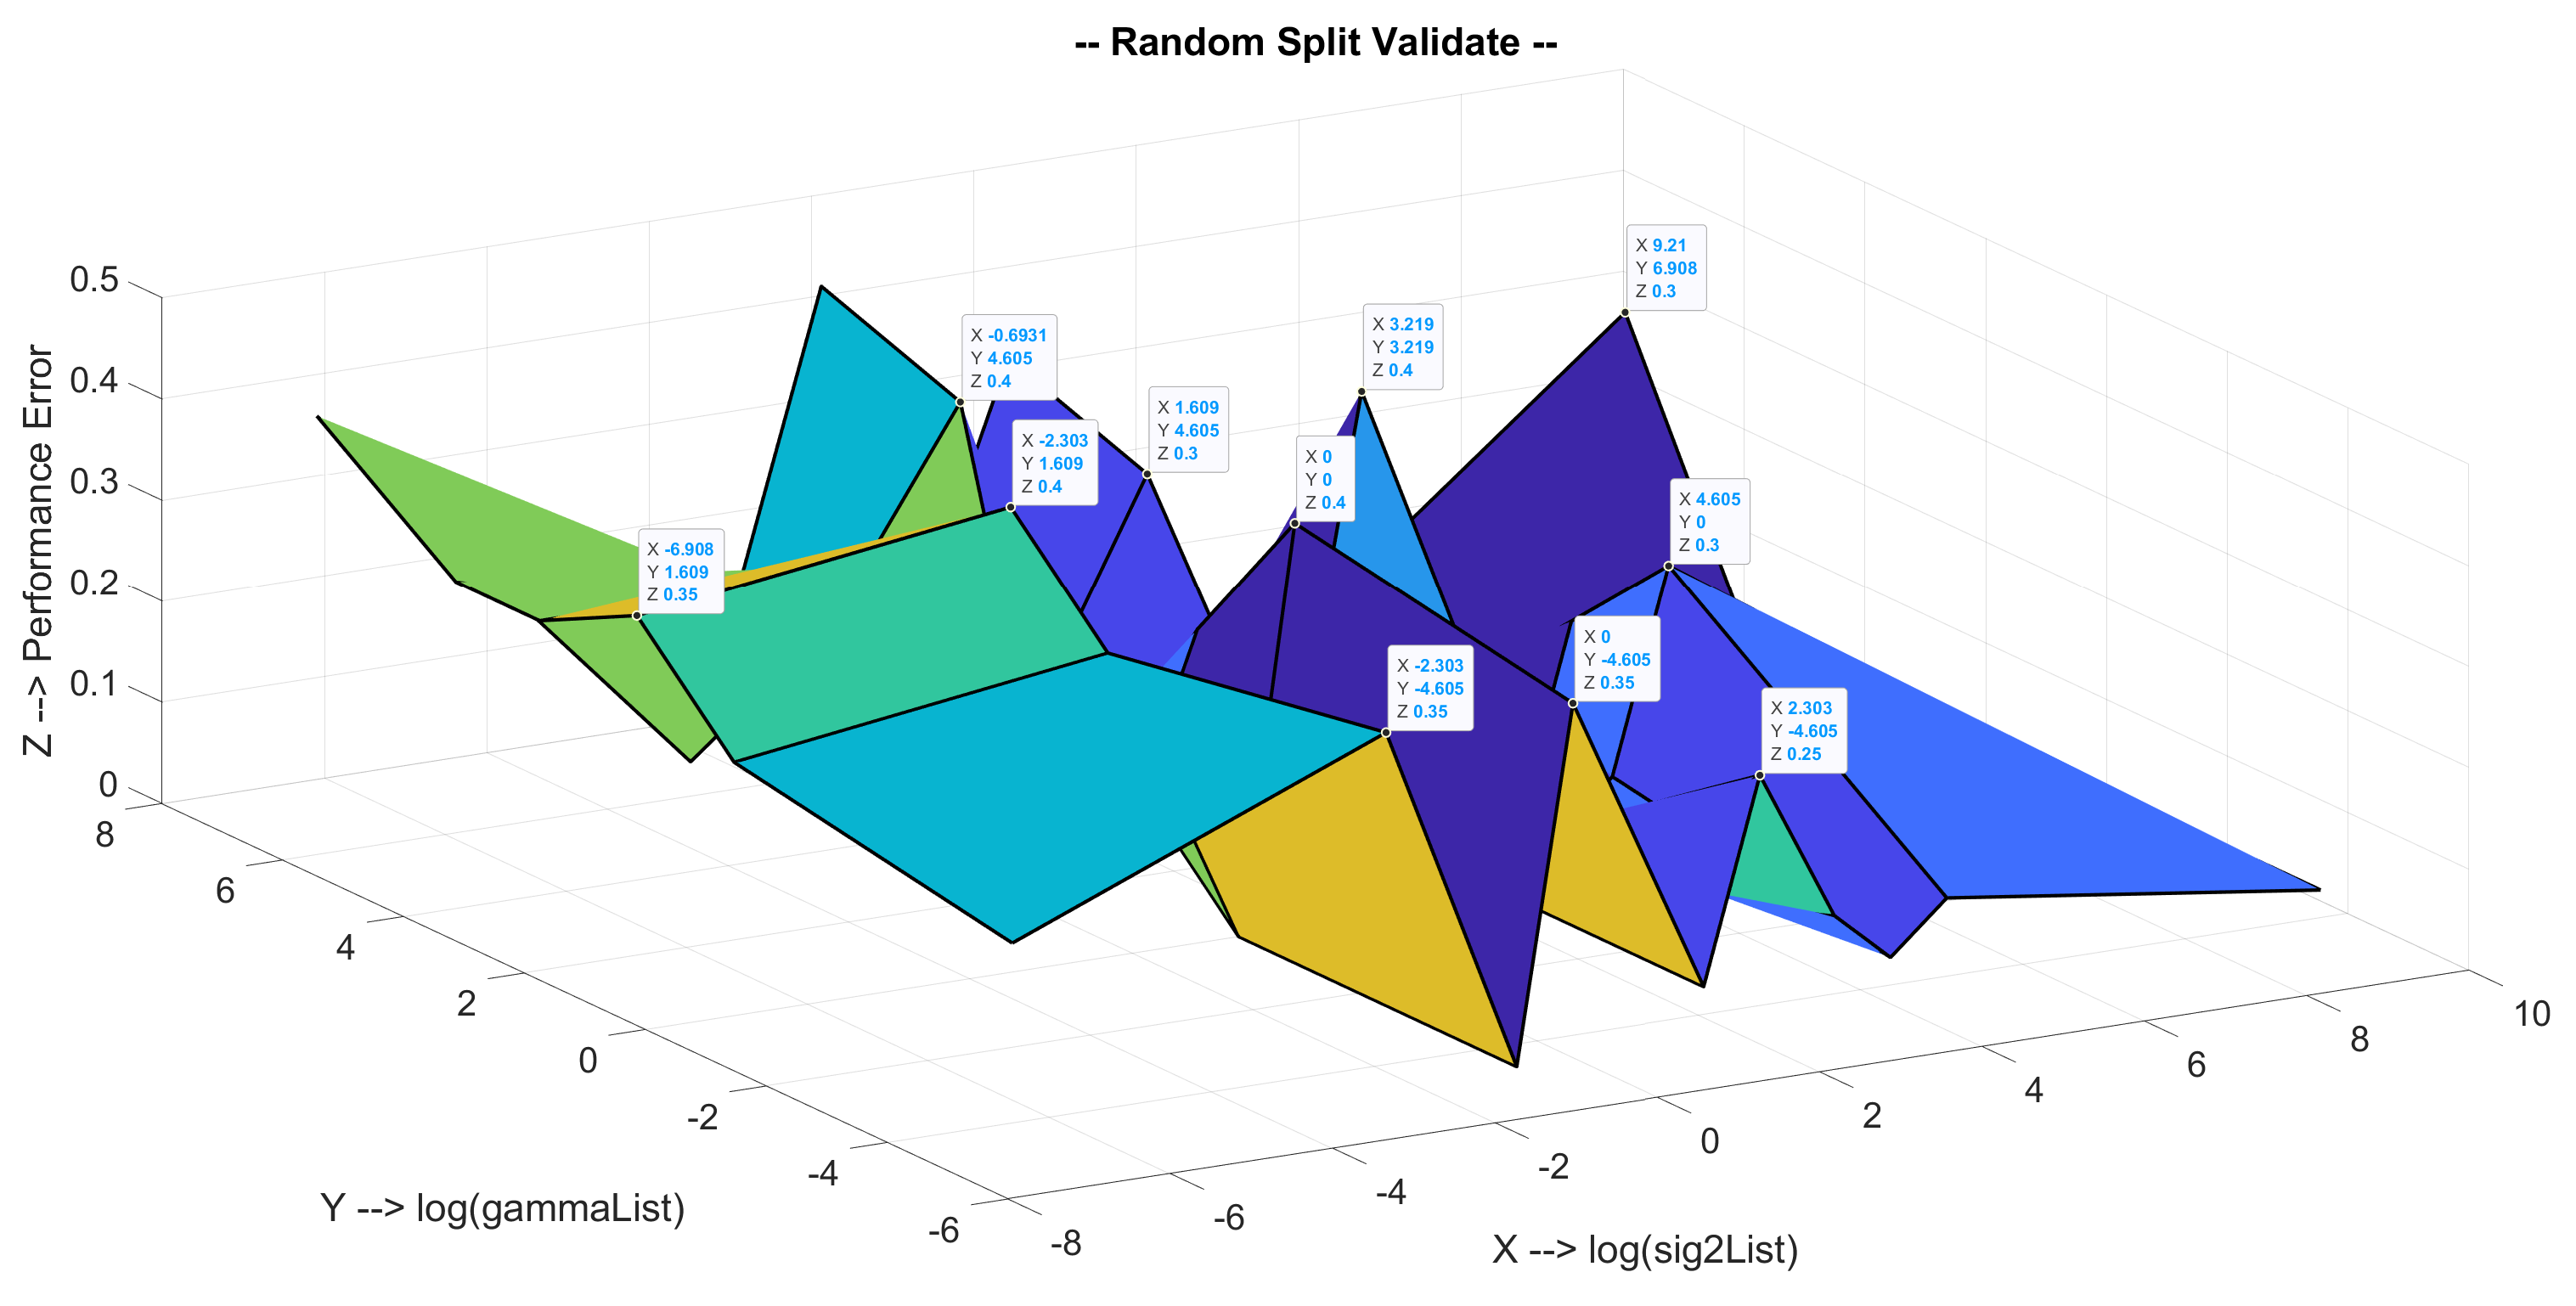
\includegraphics[height=0.8\linewidth,width= 0.8\linewidth]{Exercise1/Report/Ex1.3_rand_surf.eps} %
		}{%
			\caption{Random Split Validation - (log($\sigma^2$) vs log
				($\gamma$) vs Performane Error)}\label{fig:rand_3D}%
		}
		\ffigbox{%
		\begin{subfigure}{.3\textwidth}
			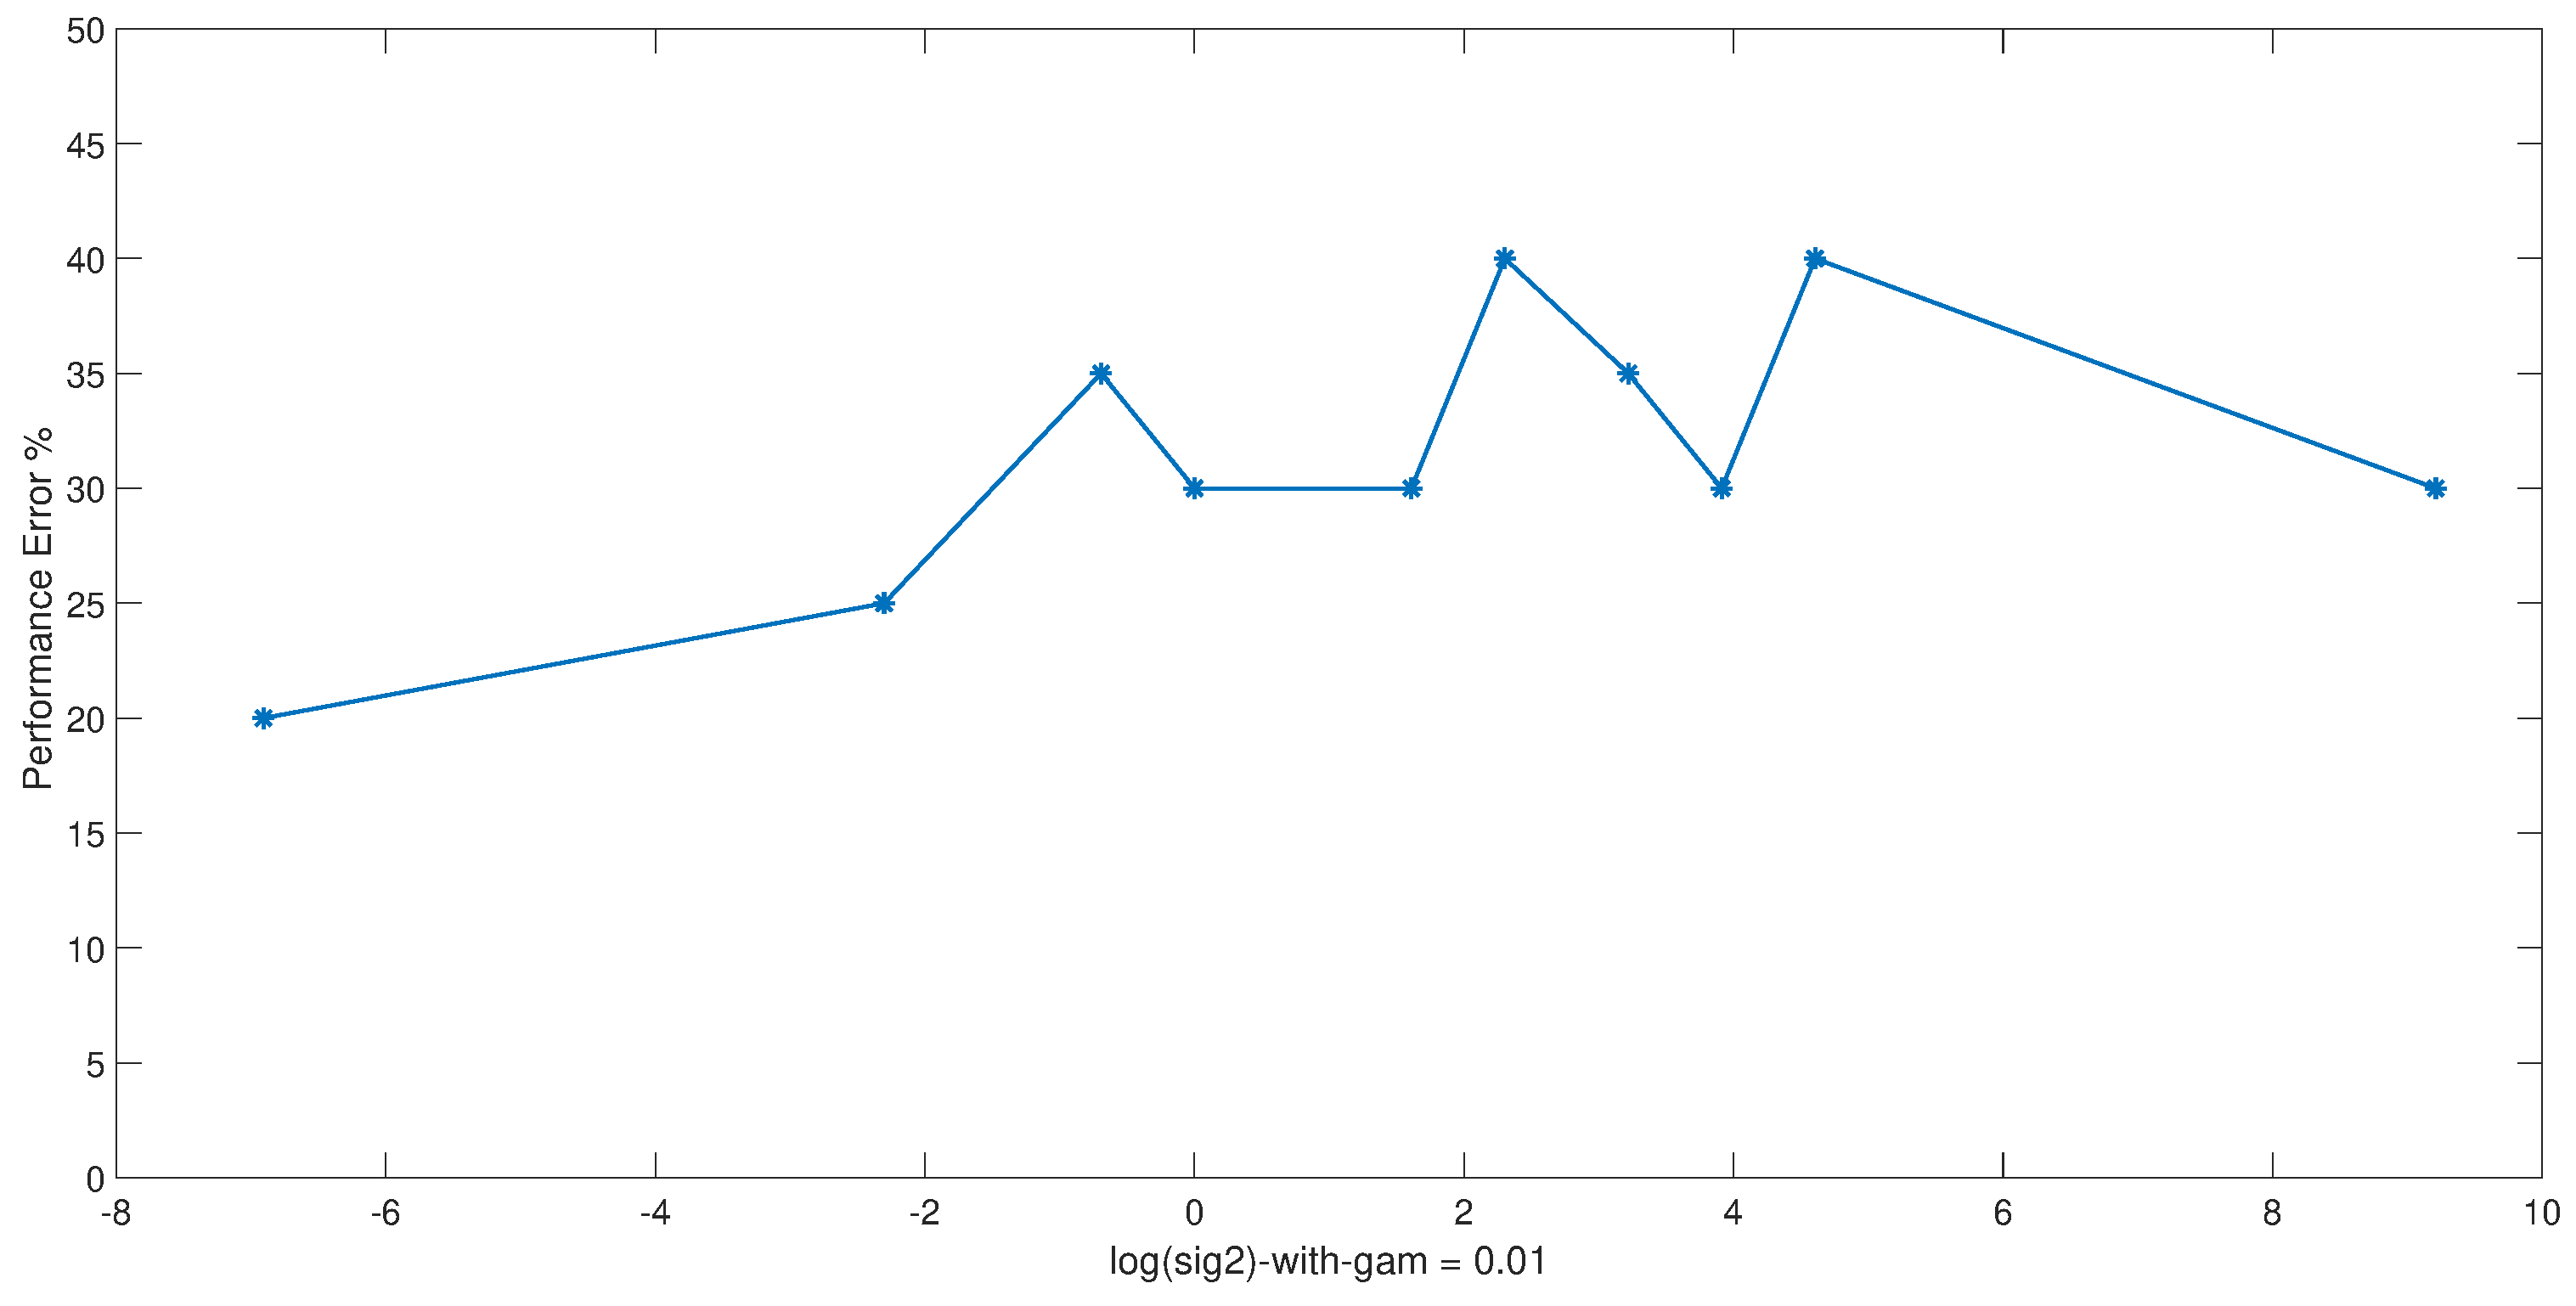
\includegraphics[height=0.35\linewidth,width=0.7\linewidth]{Exercise1/Report/Ex1.3_gam(0.01).eps}
			\caption{$\gamma$ = 0.01}
			\label{fig:rand_gamma(0.01)}
		\end{subfigure}%
		\begin{subfigure}{.3\textwidth}
			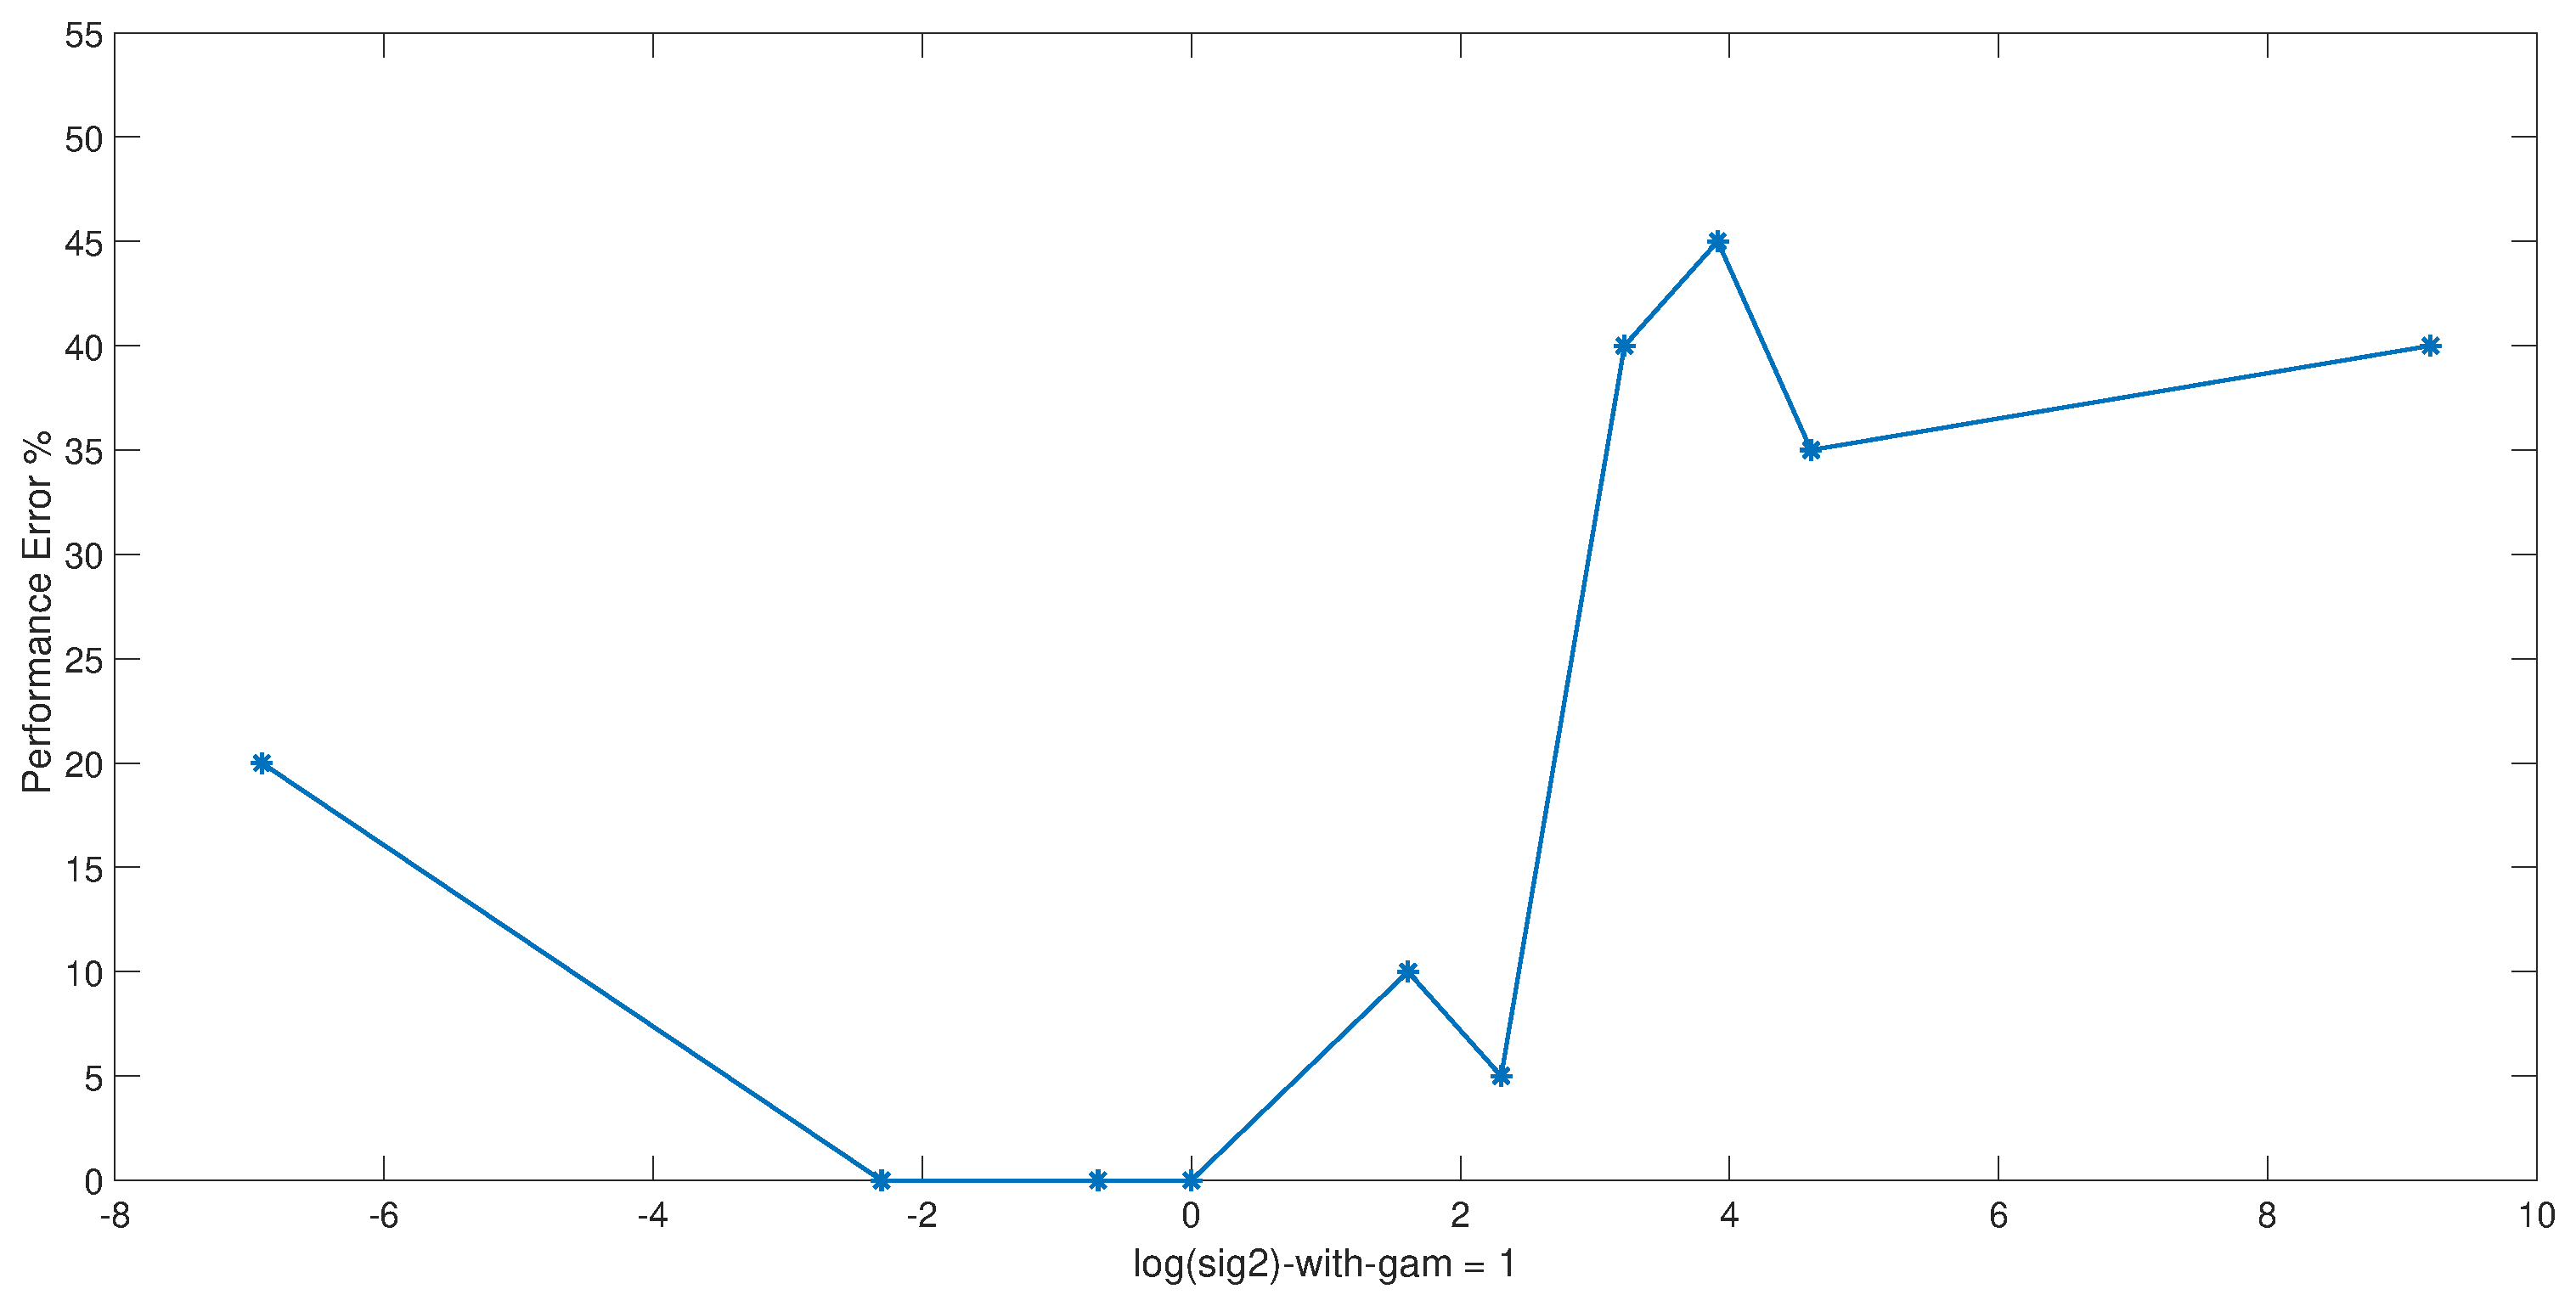
\includegraphics[height=0.35\linewidth,width=0.7\linewidth]{Exercise1/Report/Ex1.3_gam(1).eps}
			\caption{$\gamma$ = 1}
			\label{fig:rand_gamma(1))}
		\end{subfigure}
		\begin{subfigure}{.3\textwidth}
			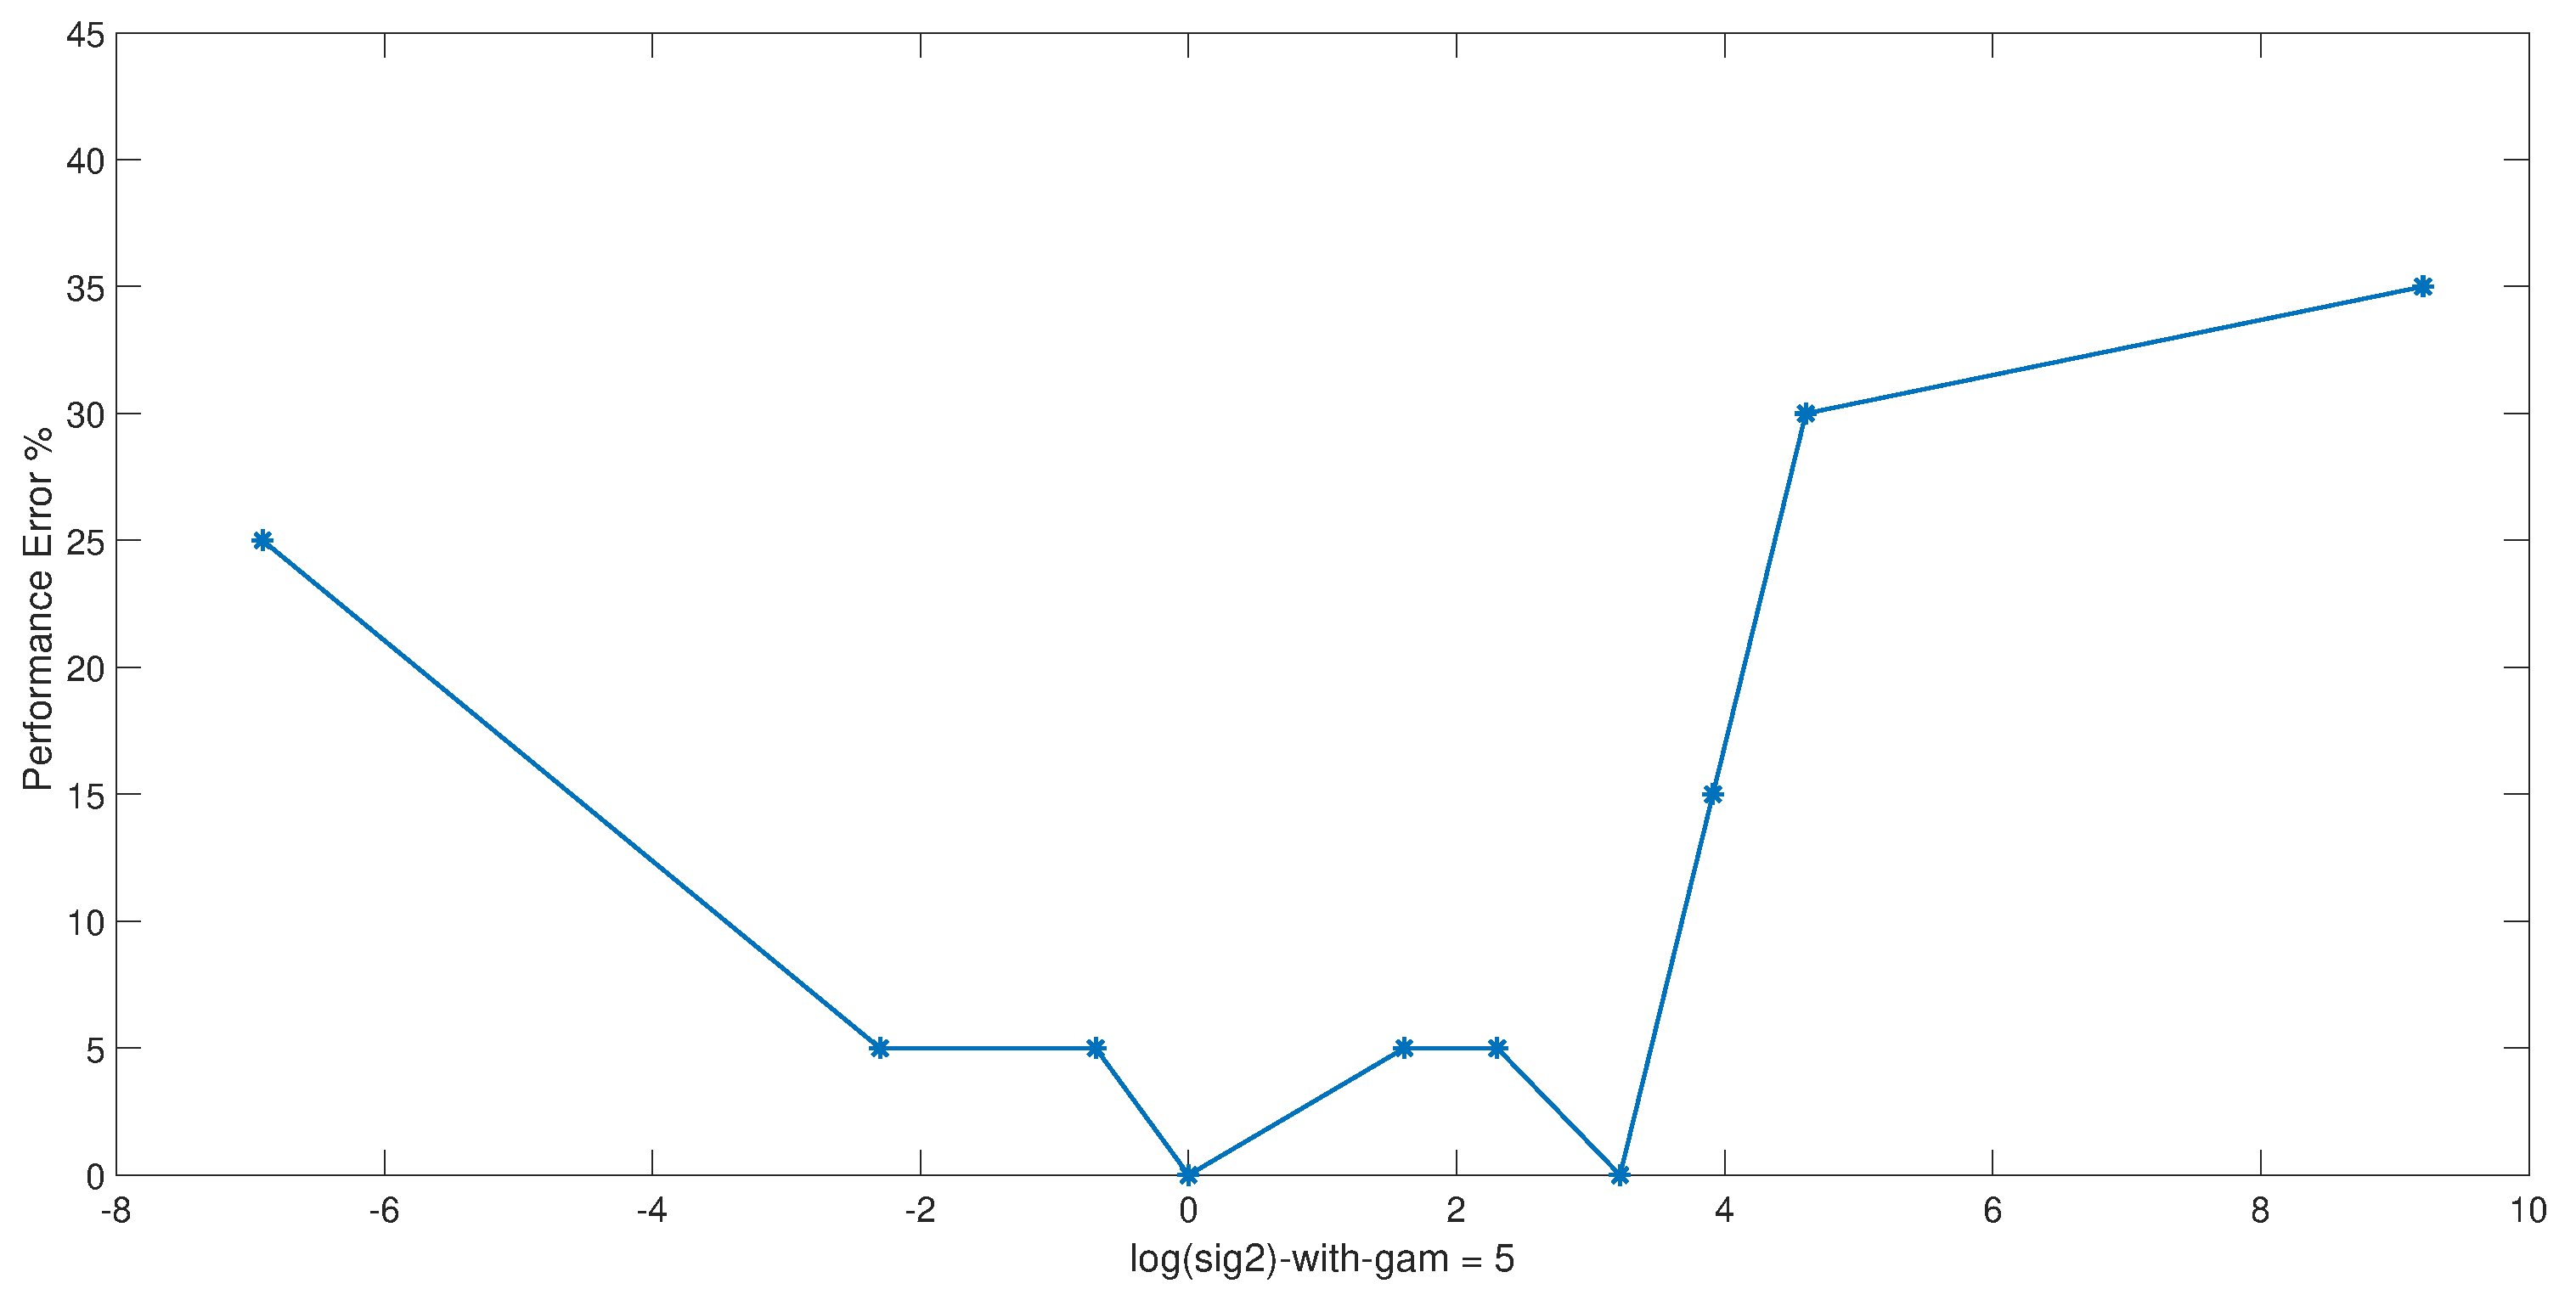
\includegraphics[height=0.35\linewidth,width=0.7\linewidth]{Exercise1/Report/Ex1.3_gam(5).eps}
			\caption{$\gamma$ = 5}
			\label{fig:rand_gamma(5)}
		\end{subfigure}%
		\begin{subfigure}{.3\textwidth}
			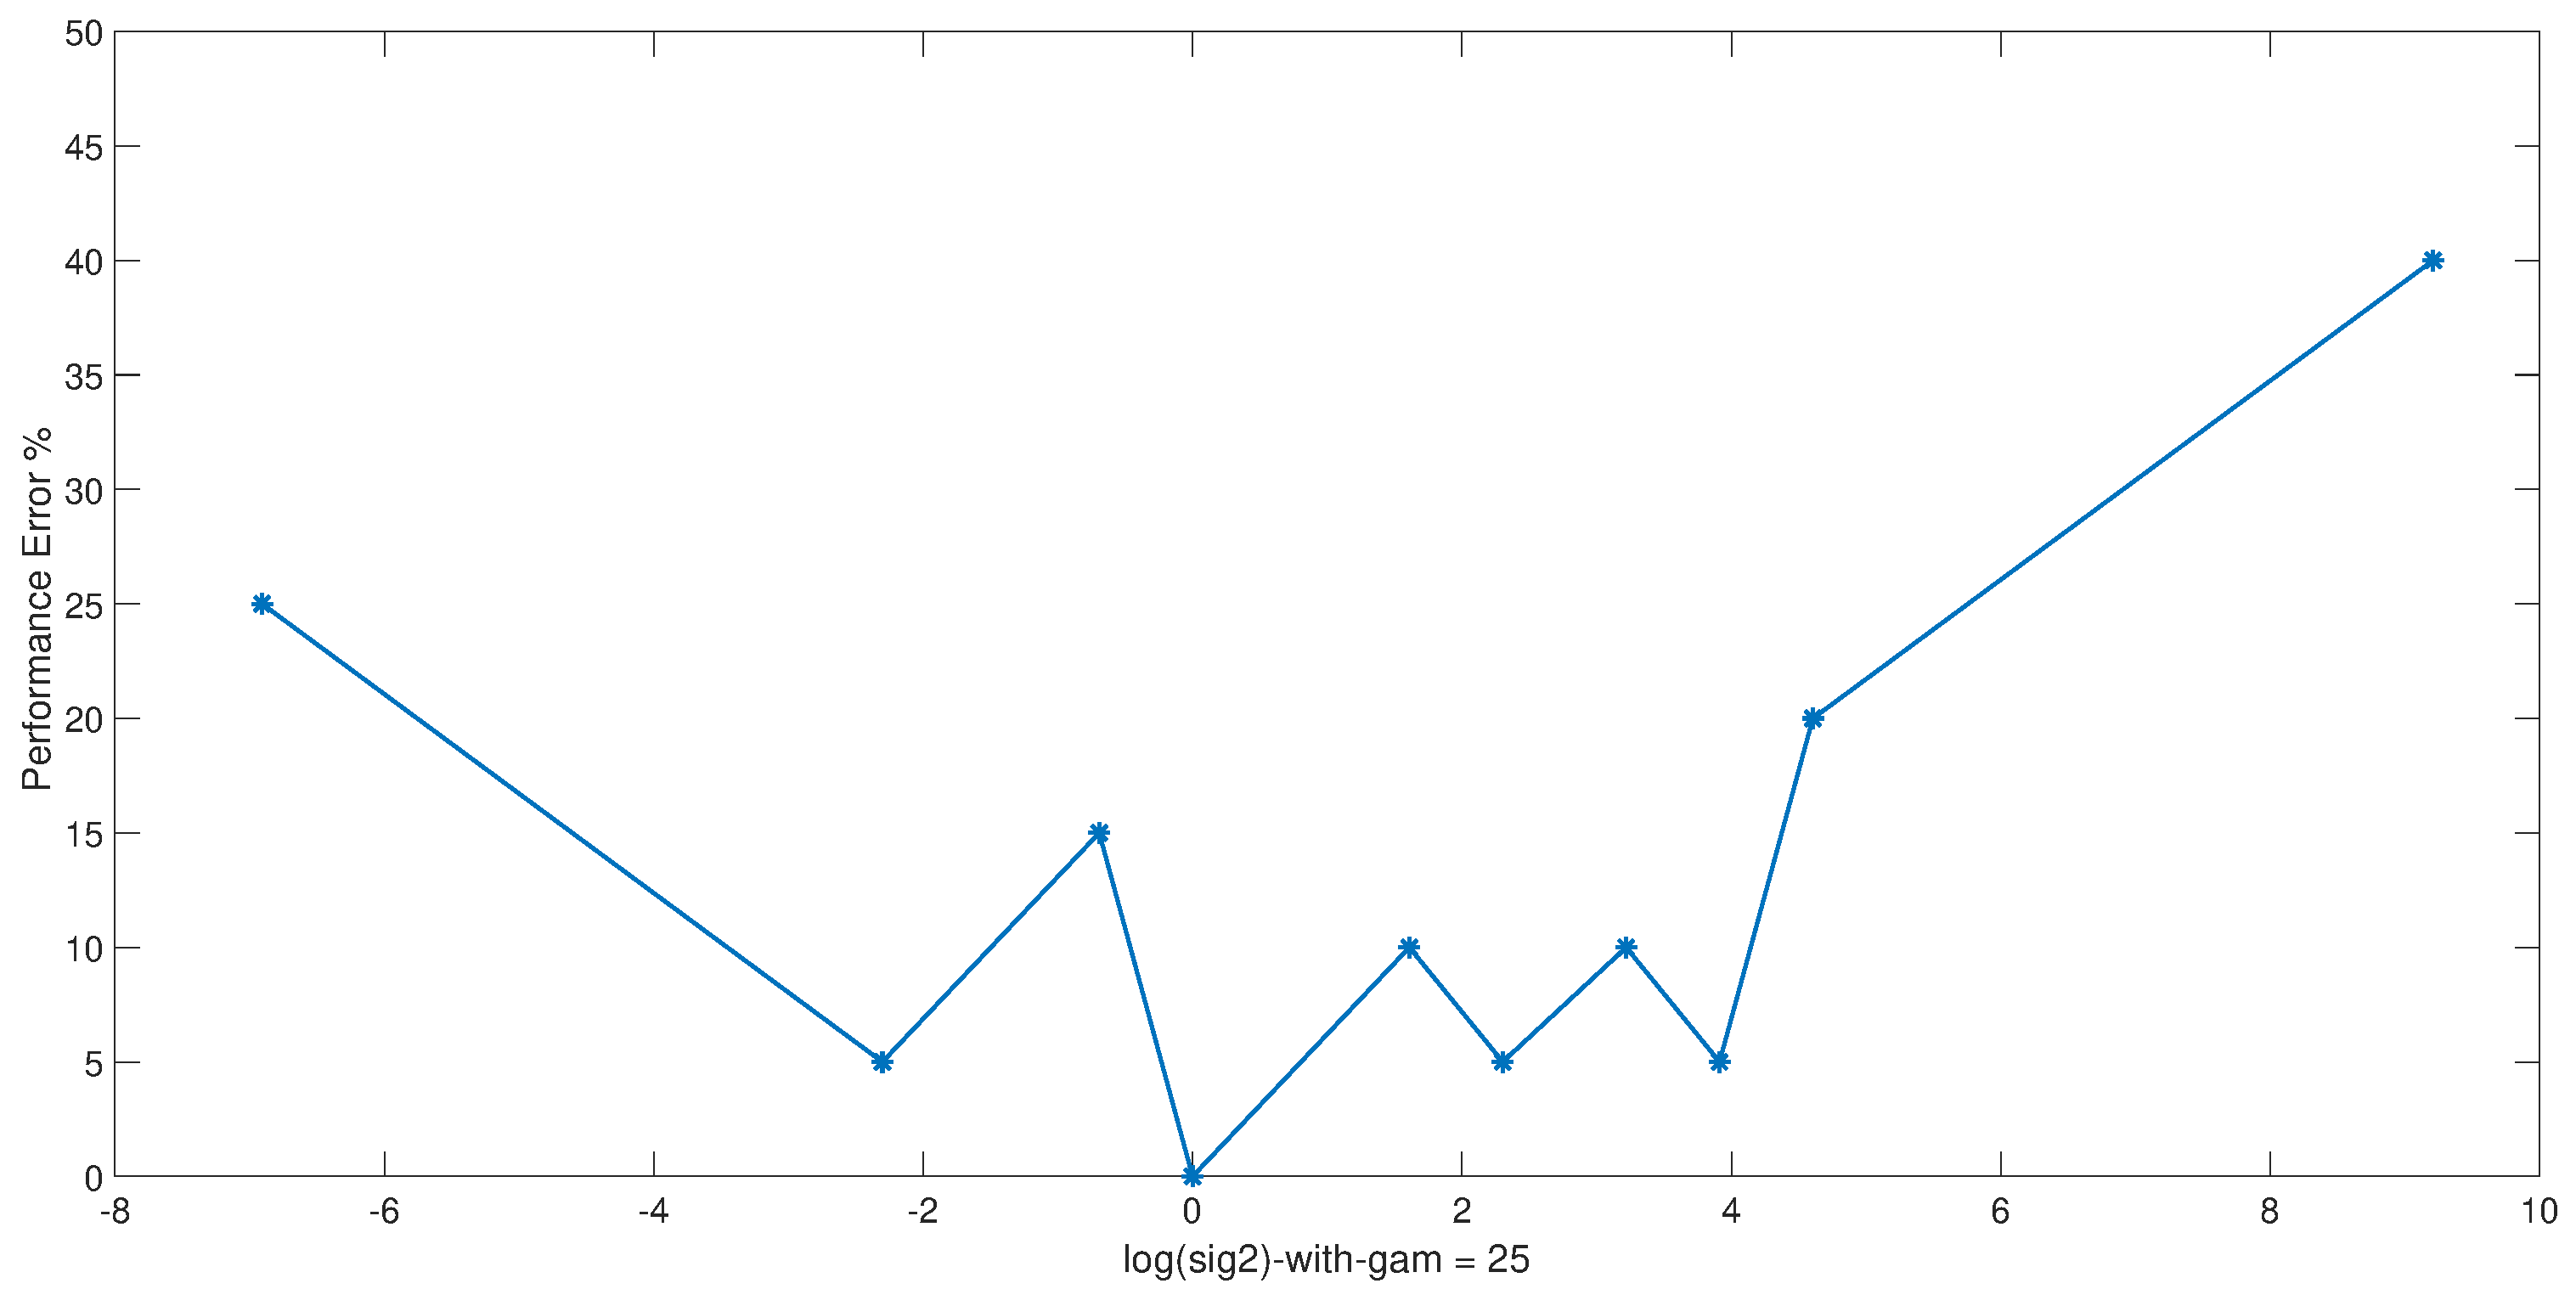
\includegraphics[height=0.35\linewidth,width=0.7\linewidth]{Exercise1/Report/Ex1.3_gam(25).eps}
			\caption{$\gamma$ = 25}
			\label{fig:rand_gamma(25)}
		\end{subfigure}
		\begin{subfigure}{.3\textwidth}
			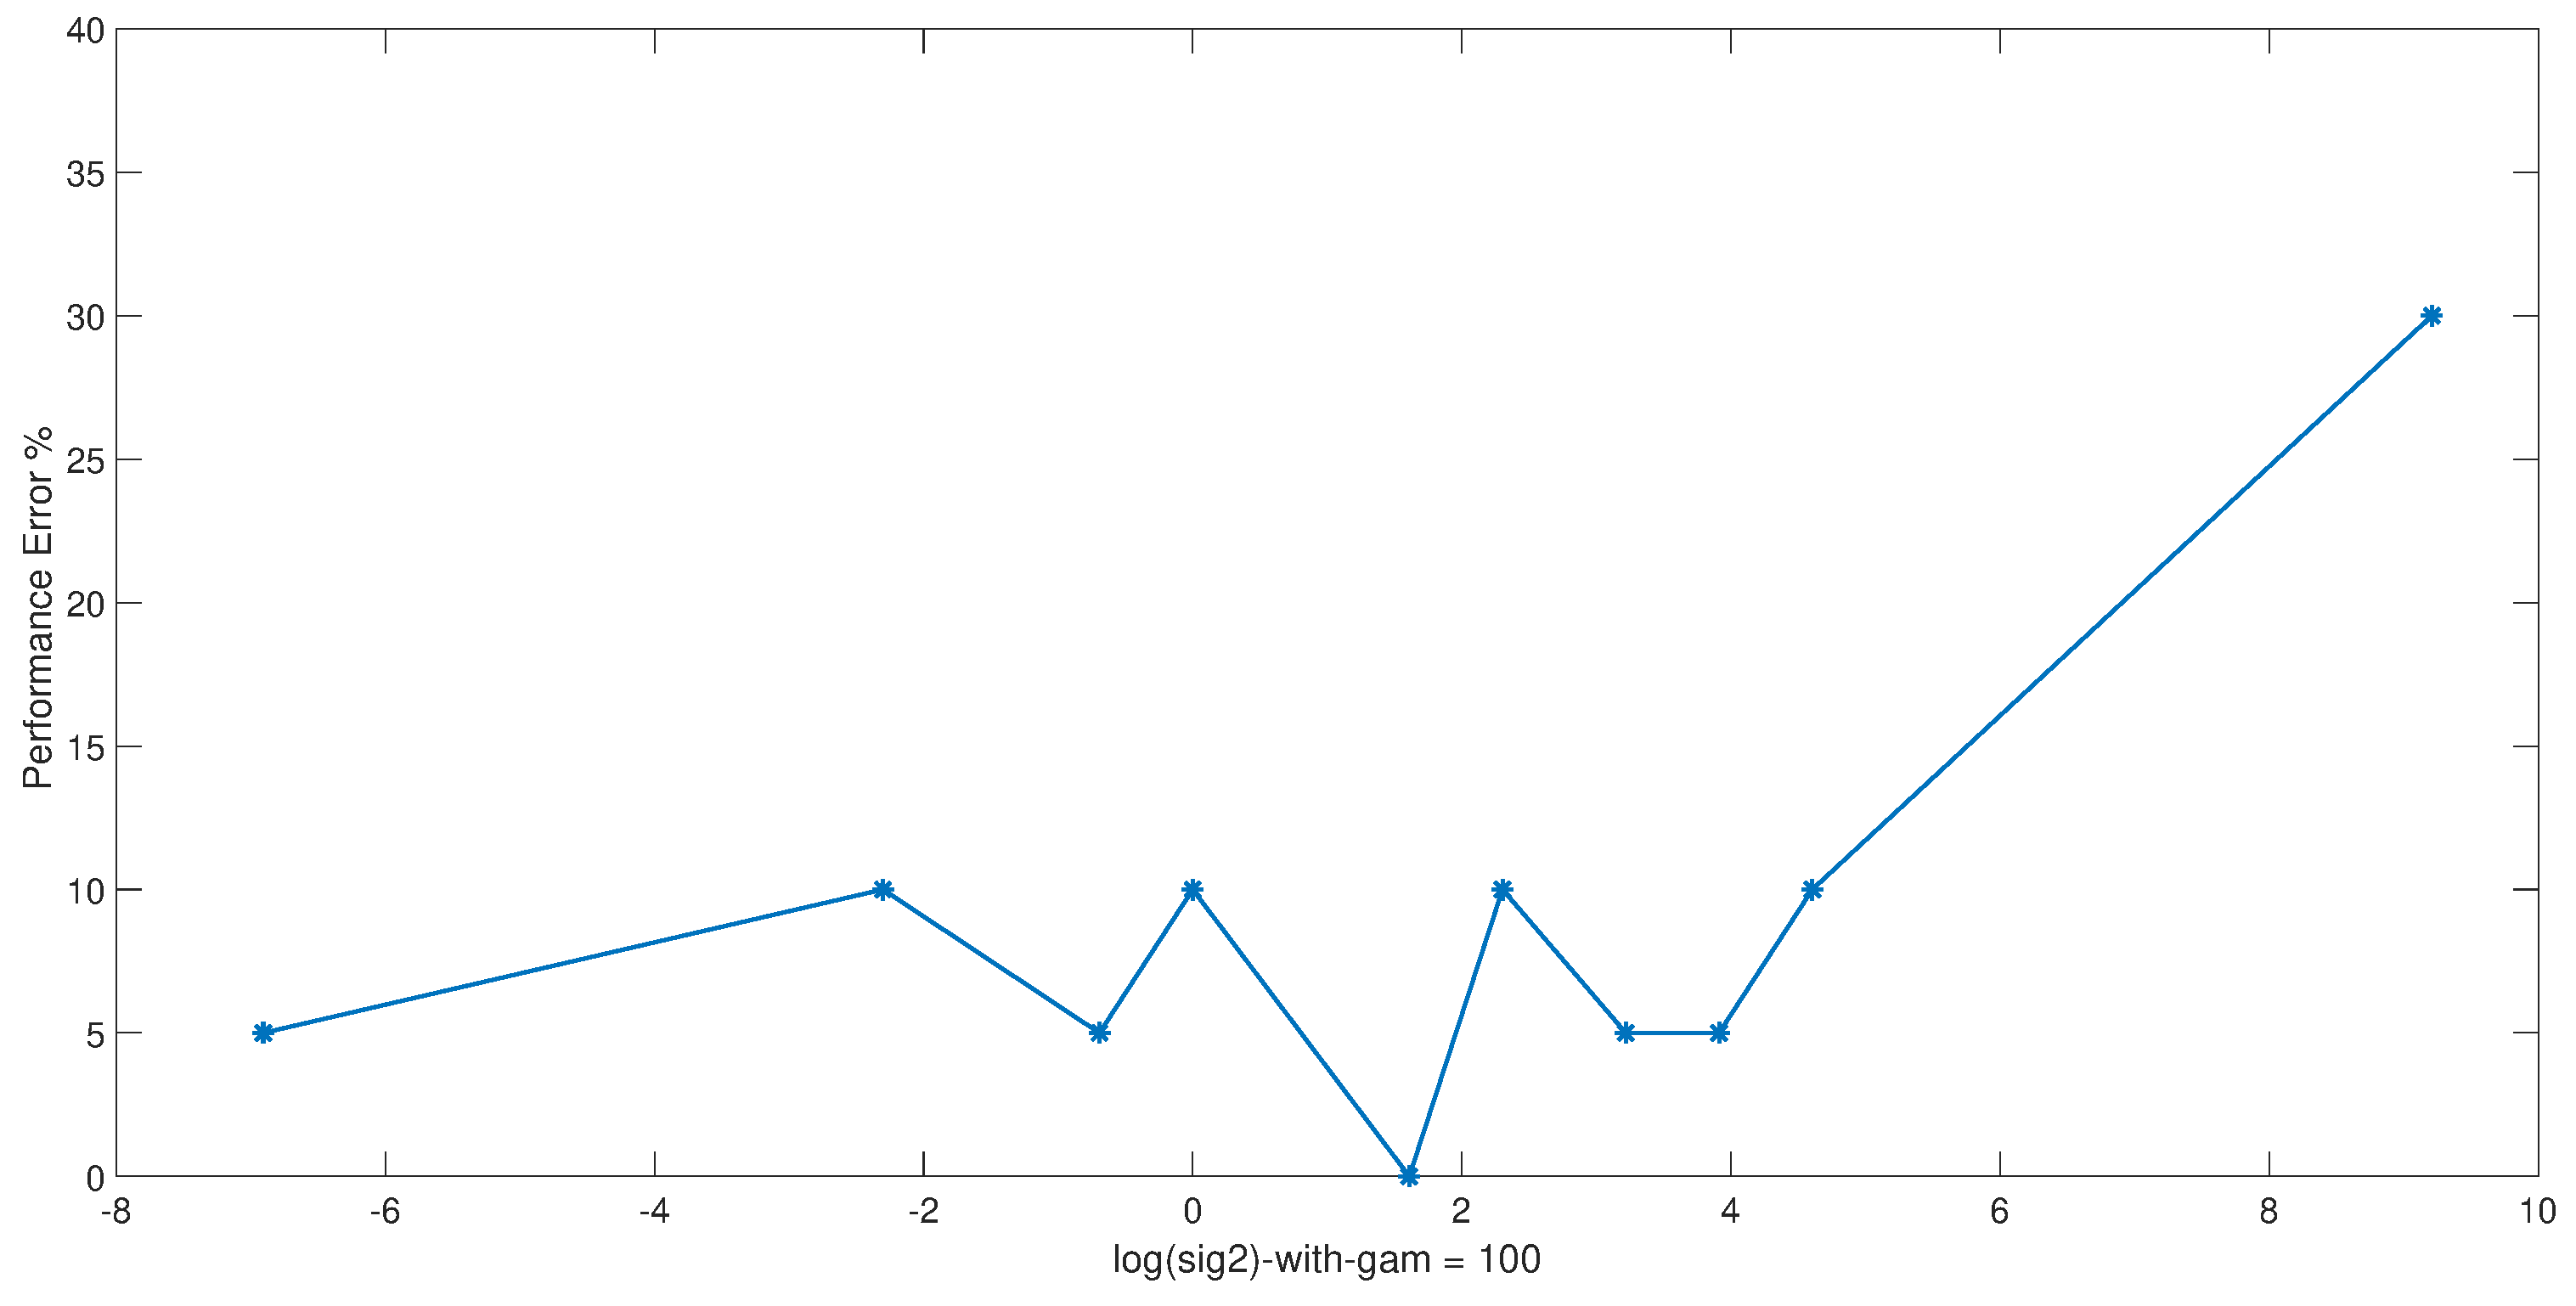
\includegraphics[height=0.35\linewidth,width=0.7\linewidth]{Exercise1/Report/Ex1.3_gam(100).eps}
			\caption{$\gamma$ = 100}
			\label{fig:rand_gamma(100)}
		\end{subfigure}%
		\begin{subfigure}{.3\textwidth}
			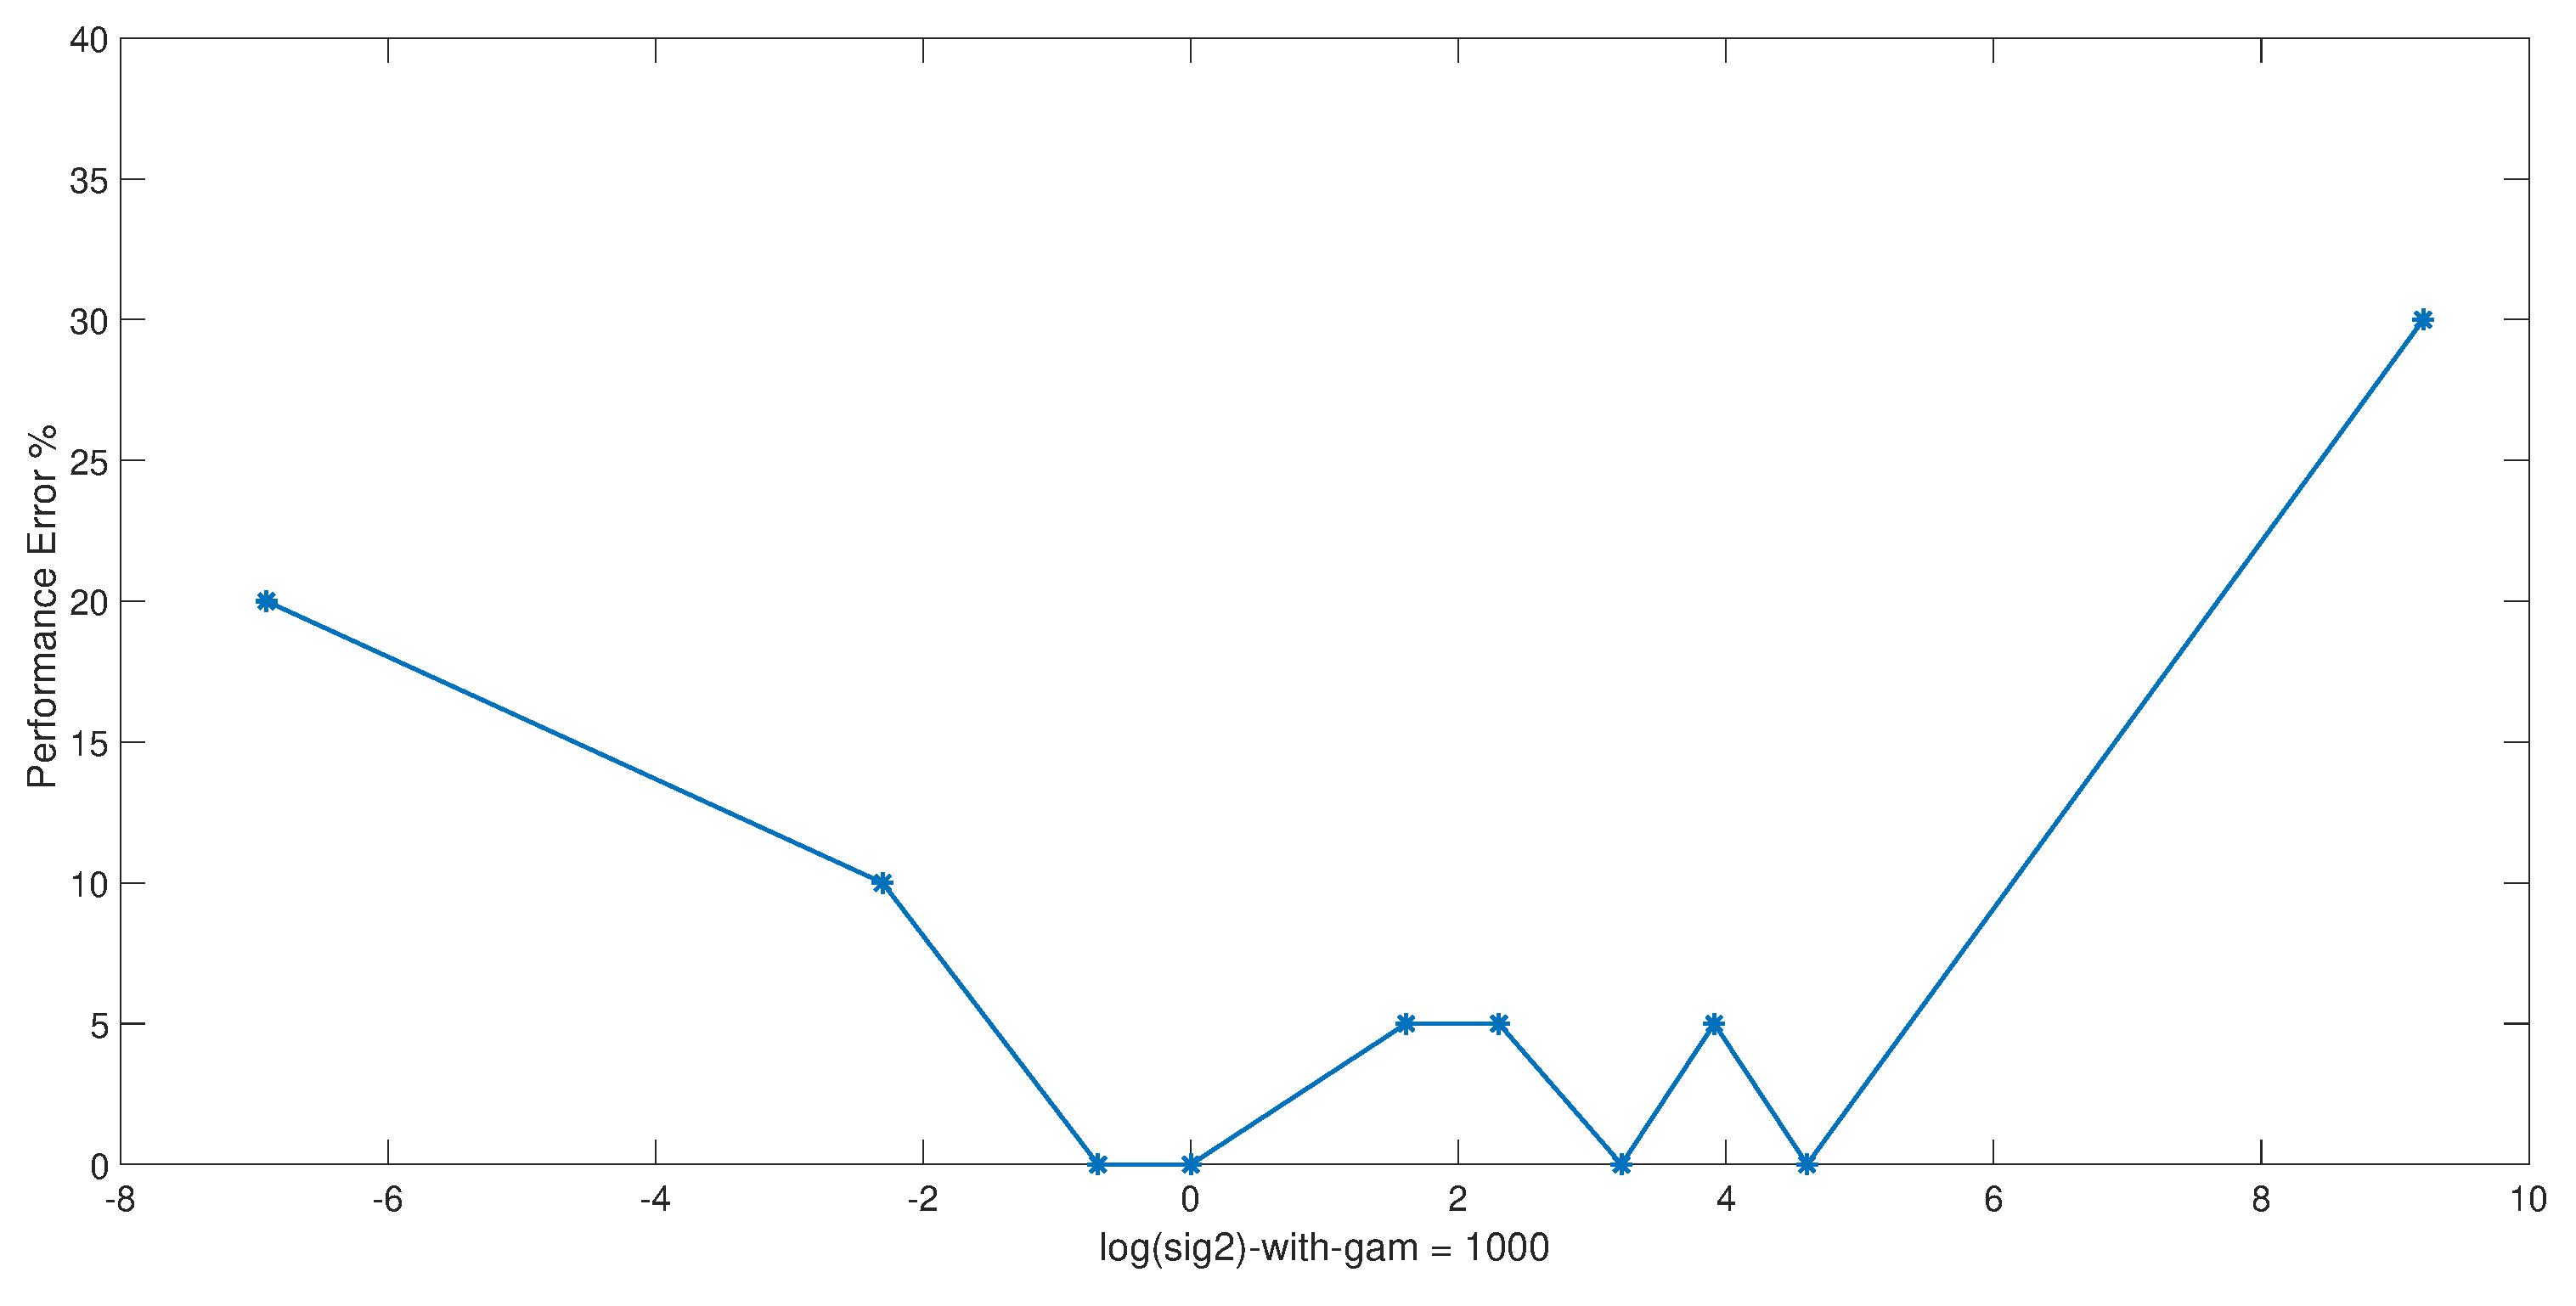
\includegraphics[height=0.35\linewidth,width=0.7\linewidth]{Exercise1/Report/Ex1.3_gam(1000).eps}
			\caption{$\gamma$ = 1000}
			\label{fig:rand_gamma(1000)}
		\end{subfigure}%			
		}{%
			\caption{Iris data : Random Split Validation (log($\sigma^2$) values for each level of $\gamma$ Vs Performance Error)  (\%) on validation set.}\label{fig:rand_gam}
		}
	\end{floatrow}
\end{figure}

We continue with the Iris data set and tune parameters of $\gamma$ and $\sigma^2$ for a range of values. We use the range of $\gamma$ as (0.01; 1; 5; 25; 100; 1000) and $\sigma^2$ as (0.001; 0.1; 0.5; 1; 5; 10; 25; 50; 100; 10000). Unlike in the previous sections, we now split the training data randomly into 80\% and 20\% as training and validation sets respectively. The SVM classifier is trained on the training data and the results are shown on the validation set. Figure \ref{fig:rand_gam}  shows the performance error (\%) of SVM for a fixed $\gamma$ and a range of $\sigma^2$. Figure \ref{fig:rand_3D} shows a 3D plot over a range of ($\gamma$, $\sigma^2$) and performance errors. It is observed from figure \ref{fig:rand_gam} that the performance error varies between 20 to 40 percent for the given range of ($\gamma$, $\sigma^2$). Using these results it is difficult to determine a best performing $\gamma$ and $\sigma$ values for the random split technique.  Another way to determine a good range of ($\gamma$, $\sigma^2$) is using k-fold cross validation and leave-one-out validation.

 \begin{figure}[!ht]
	\begin{floatrow}
		\ffigbox{%
			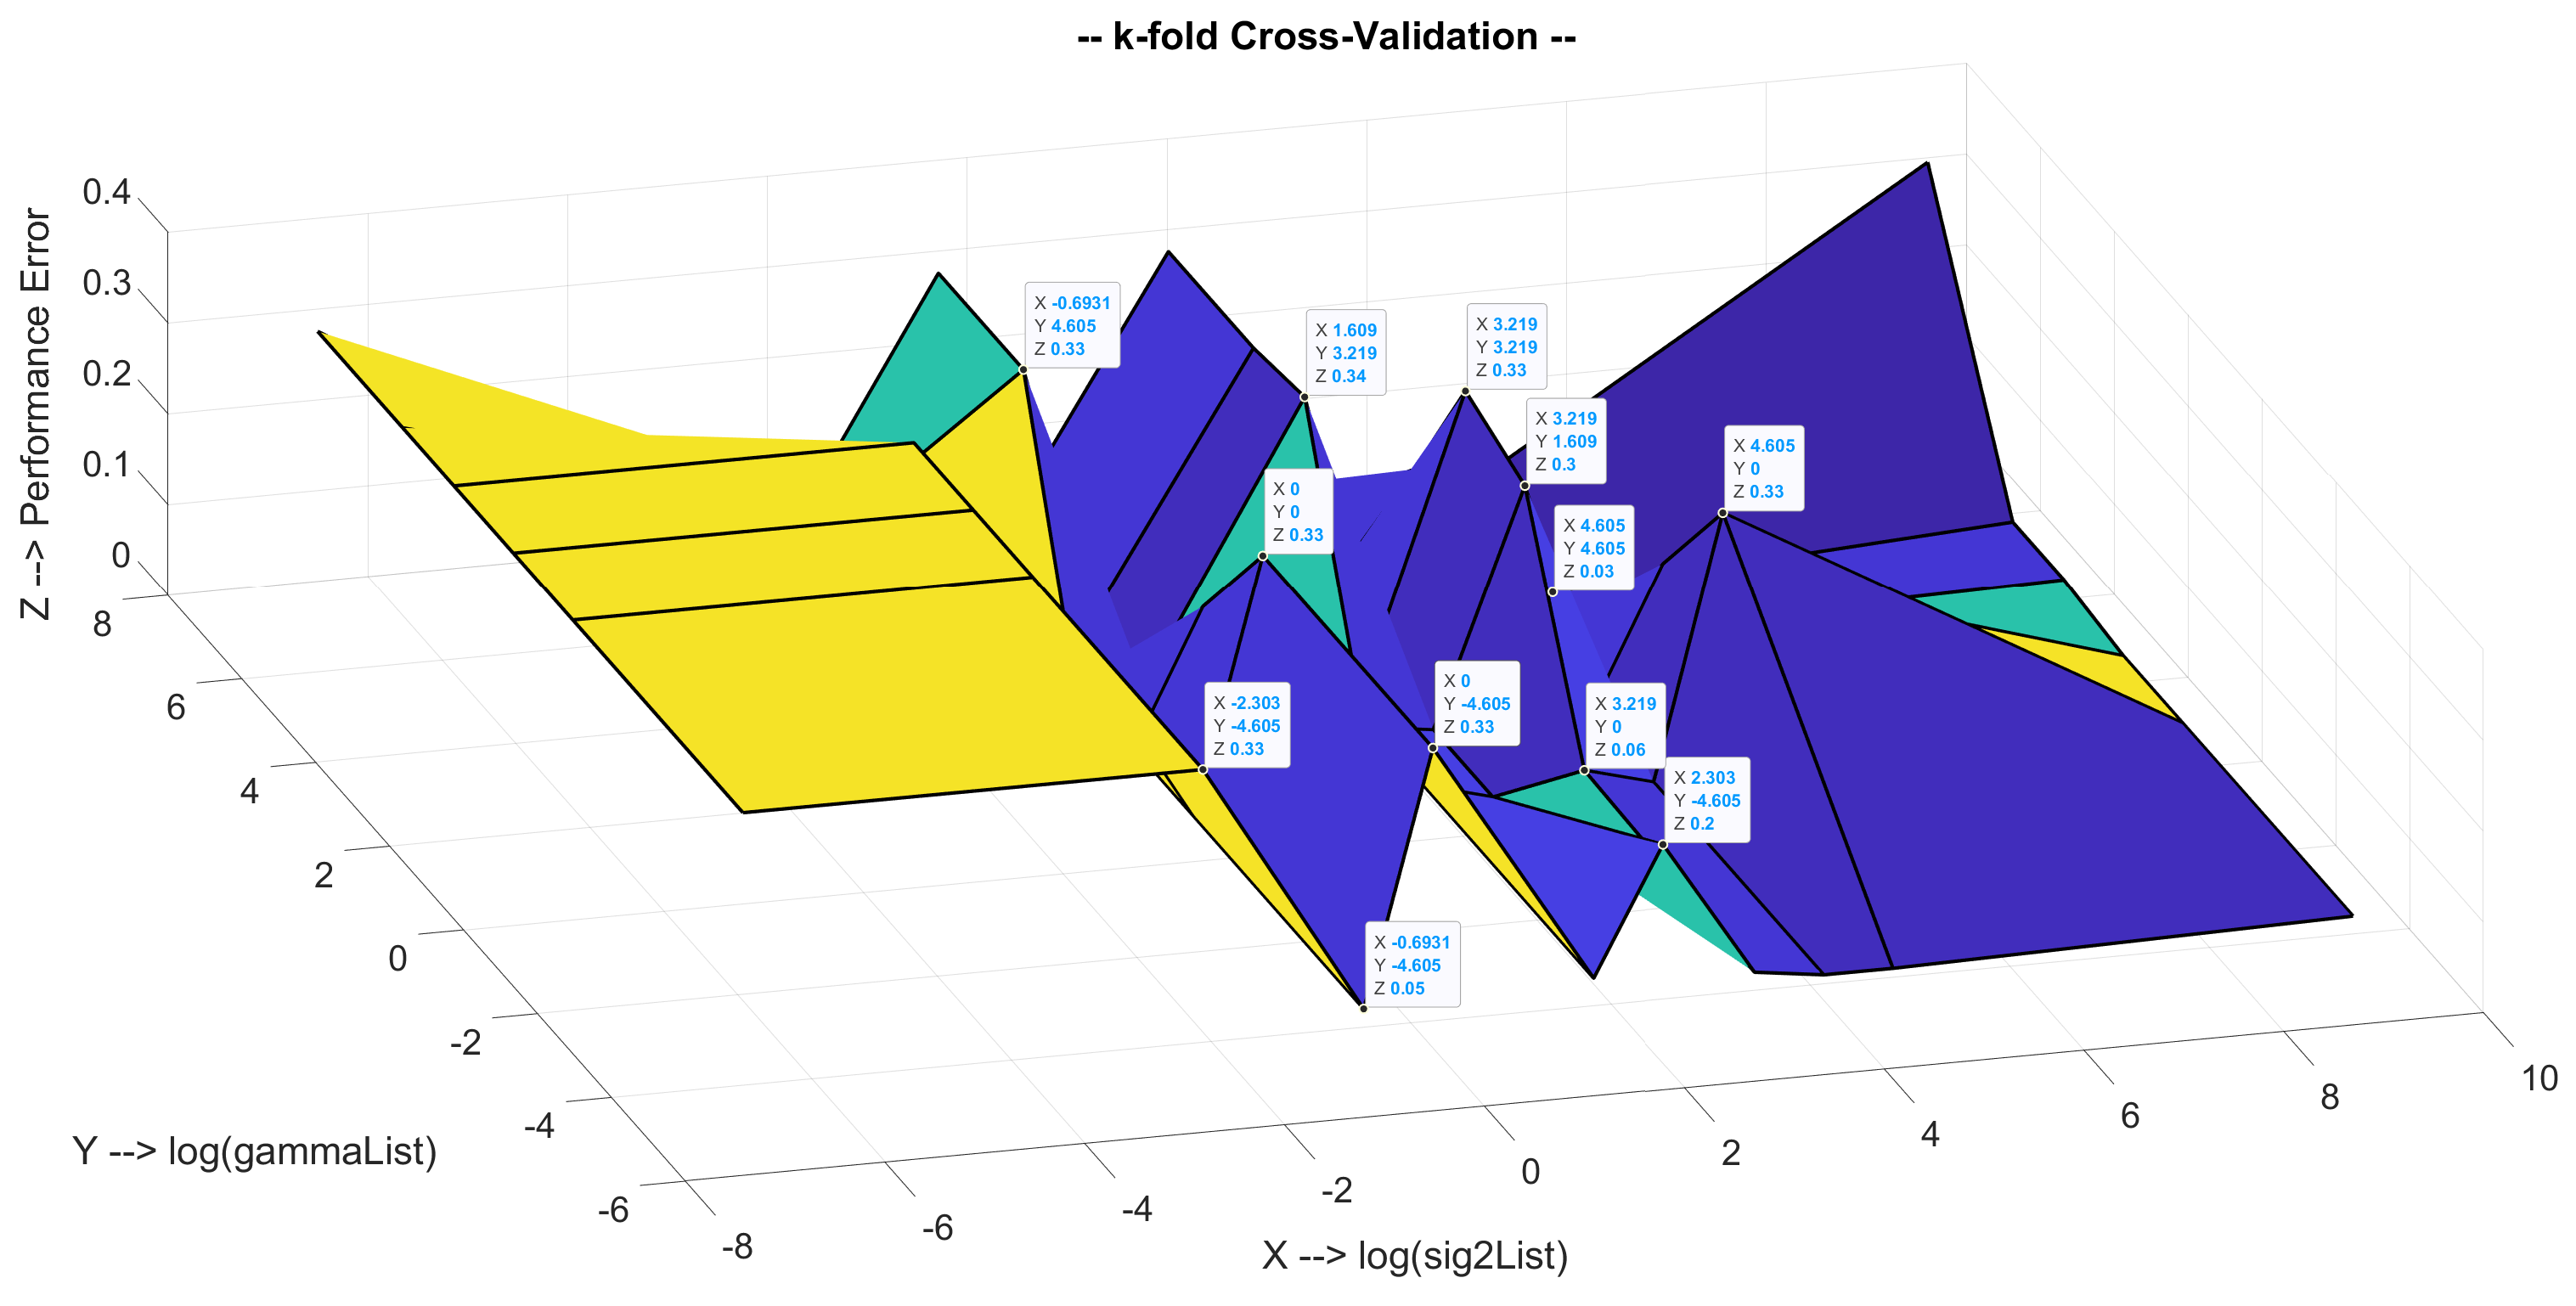
\includegraphics[height=0.8\linewidth,width= 0.8\linewidth]{Exercise1/Report/Ex1.3_kCV_surf.eps} %
		}{%
			\caption{k-fold Cross Validation - (log($\sigma^2$) vs log
				($\gamma$) vs Performane Error)}\label{fig:kCV_3D}%
		}
		\ffigbox{%
			\begin{subfigure}{.3\textwidth}
				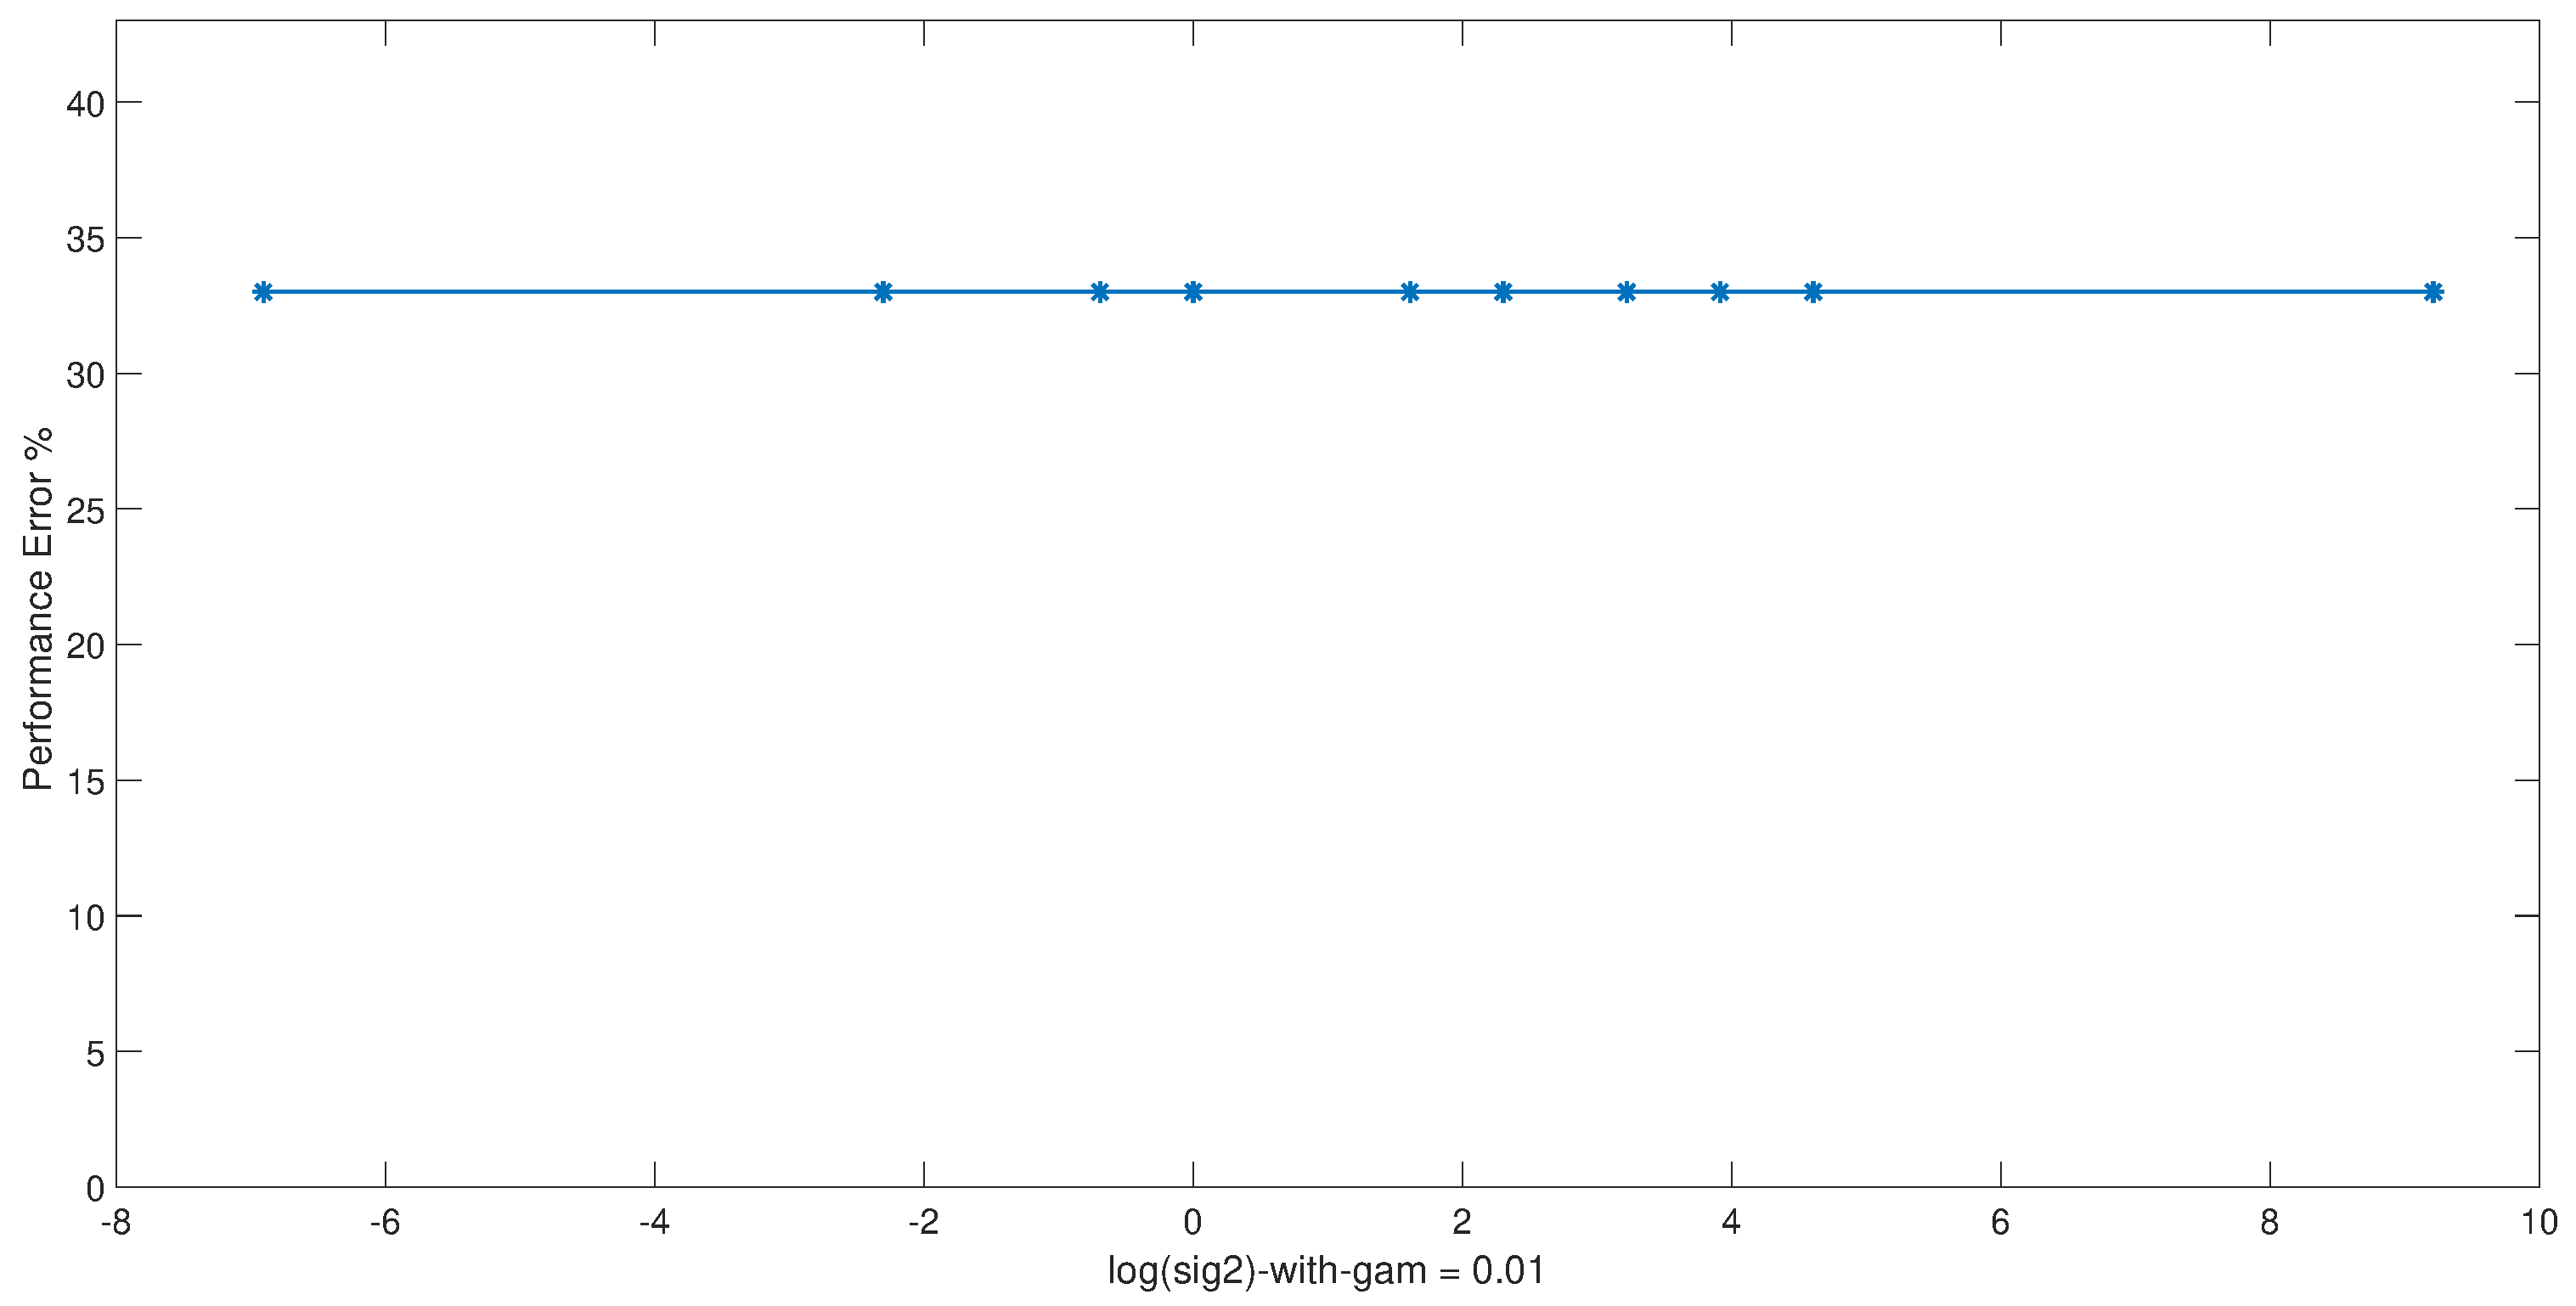
\includegraphics[height=0.35\linewidth,width=0.7\linewidth]{Exercise1/Report/Ex1.3_kCV_gam(0.01).eps}
				\caption{$\gamma$ = 0.01}
				\label{fig:kCV_gamma(0.01)}
			\end{subfigure}%
			\begin{subfigure}{.3\textwidth}
				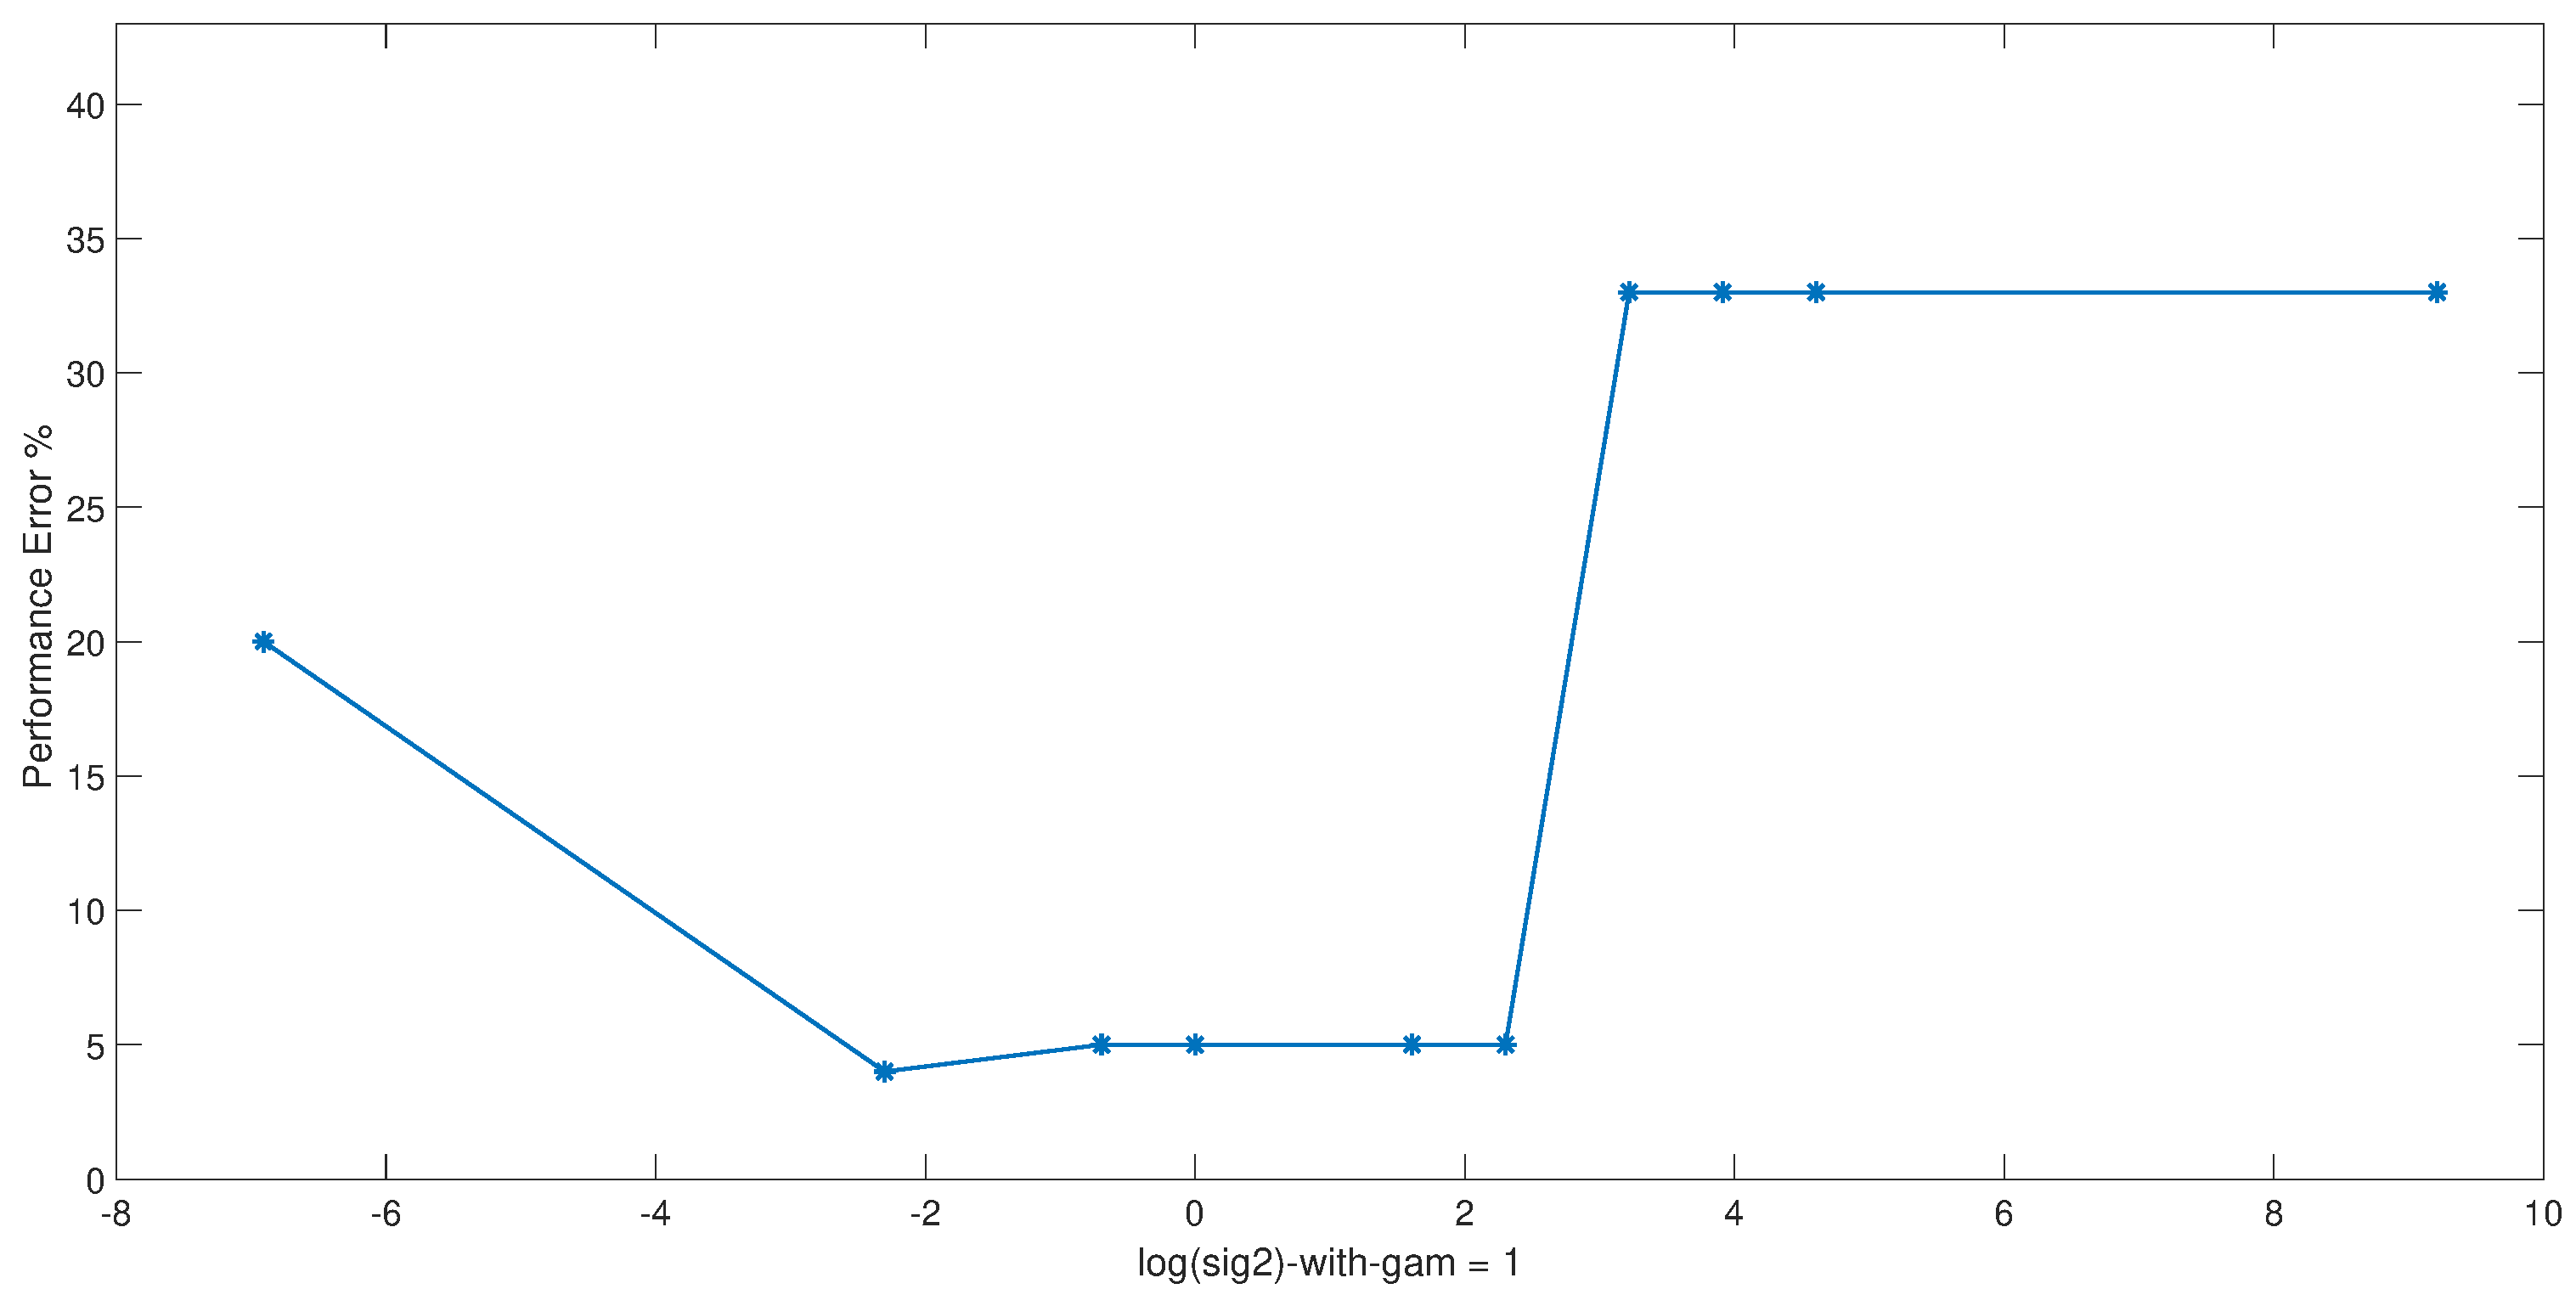
\includegraphics[height=0.35\linewidth,width=0.7\linewidth]{Exercise1/Report/Ex1.3_kCV_gam(1).eps}
				\caption{$\gamma$ = 1}
				\label{fig:kCV_gamma(1))}
			\end{subfigure}
			\begin{subfigure}{.3\textwidth}
				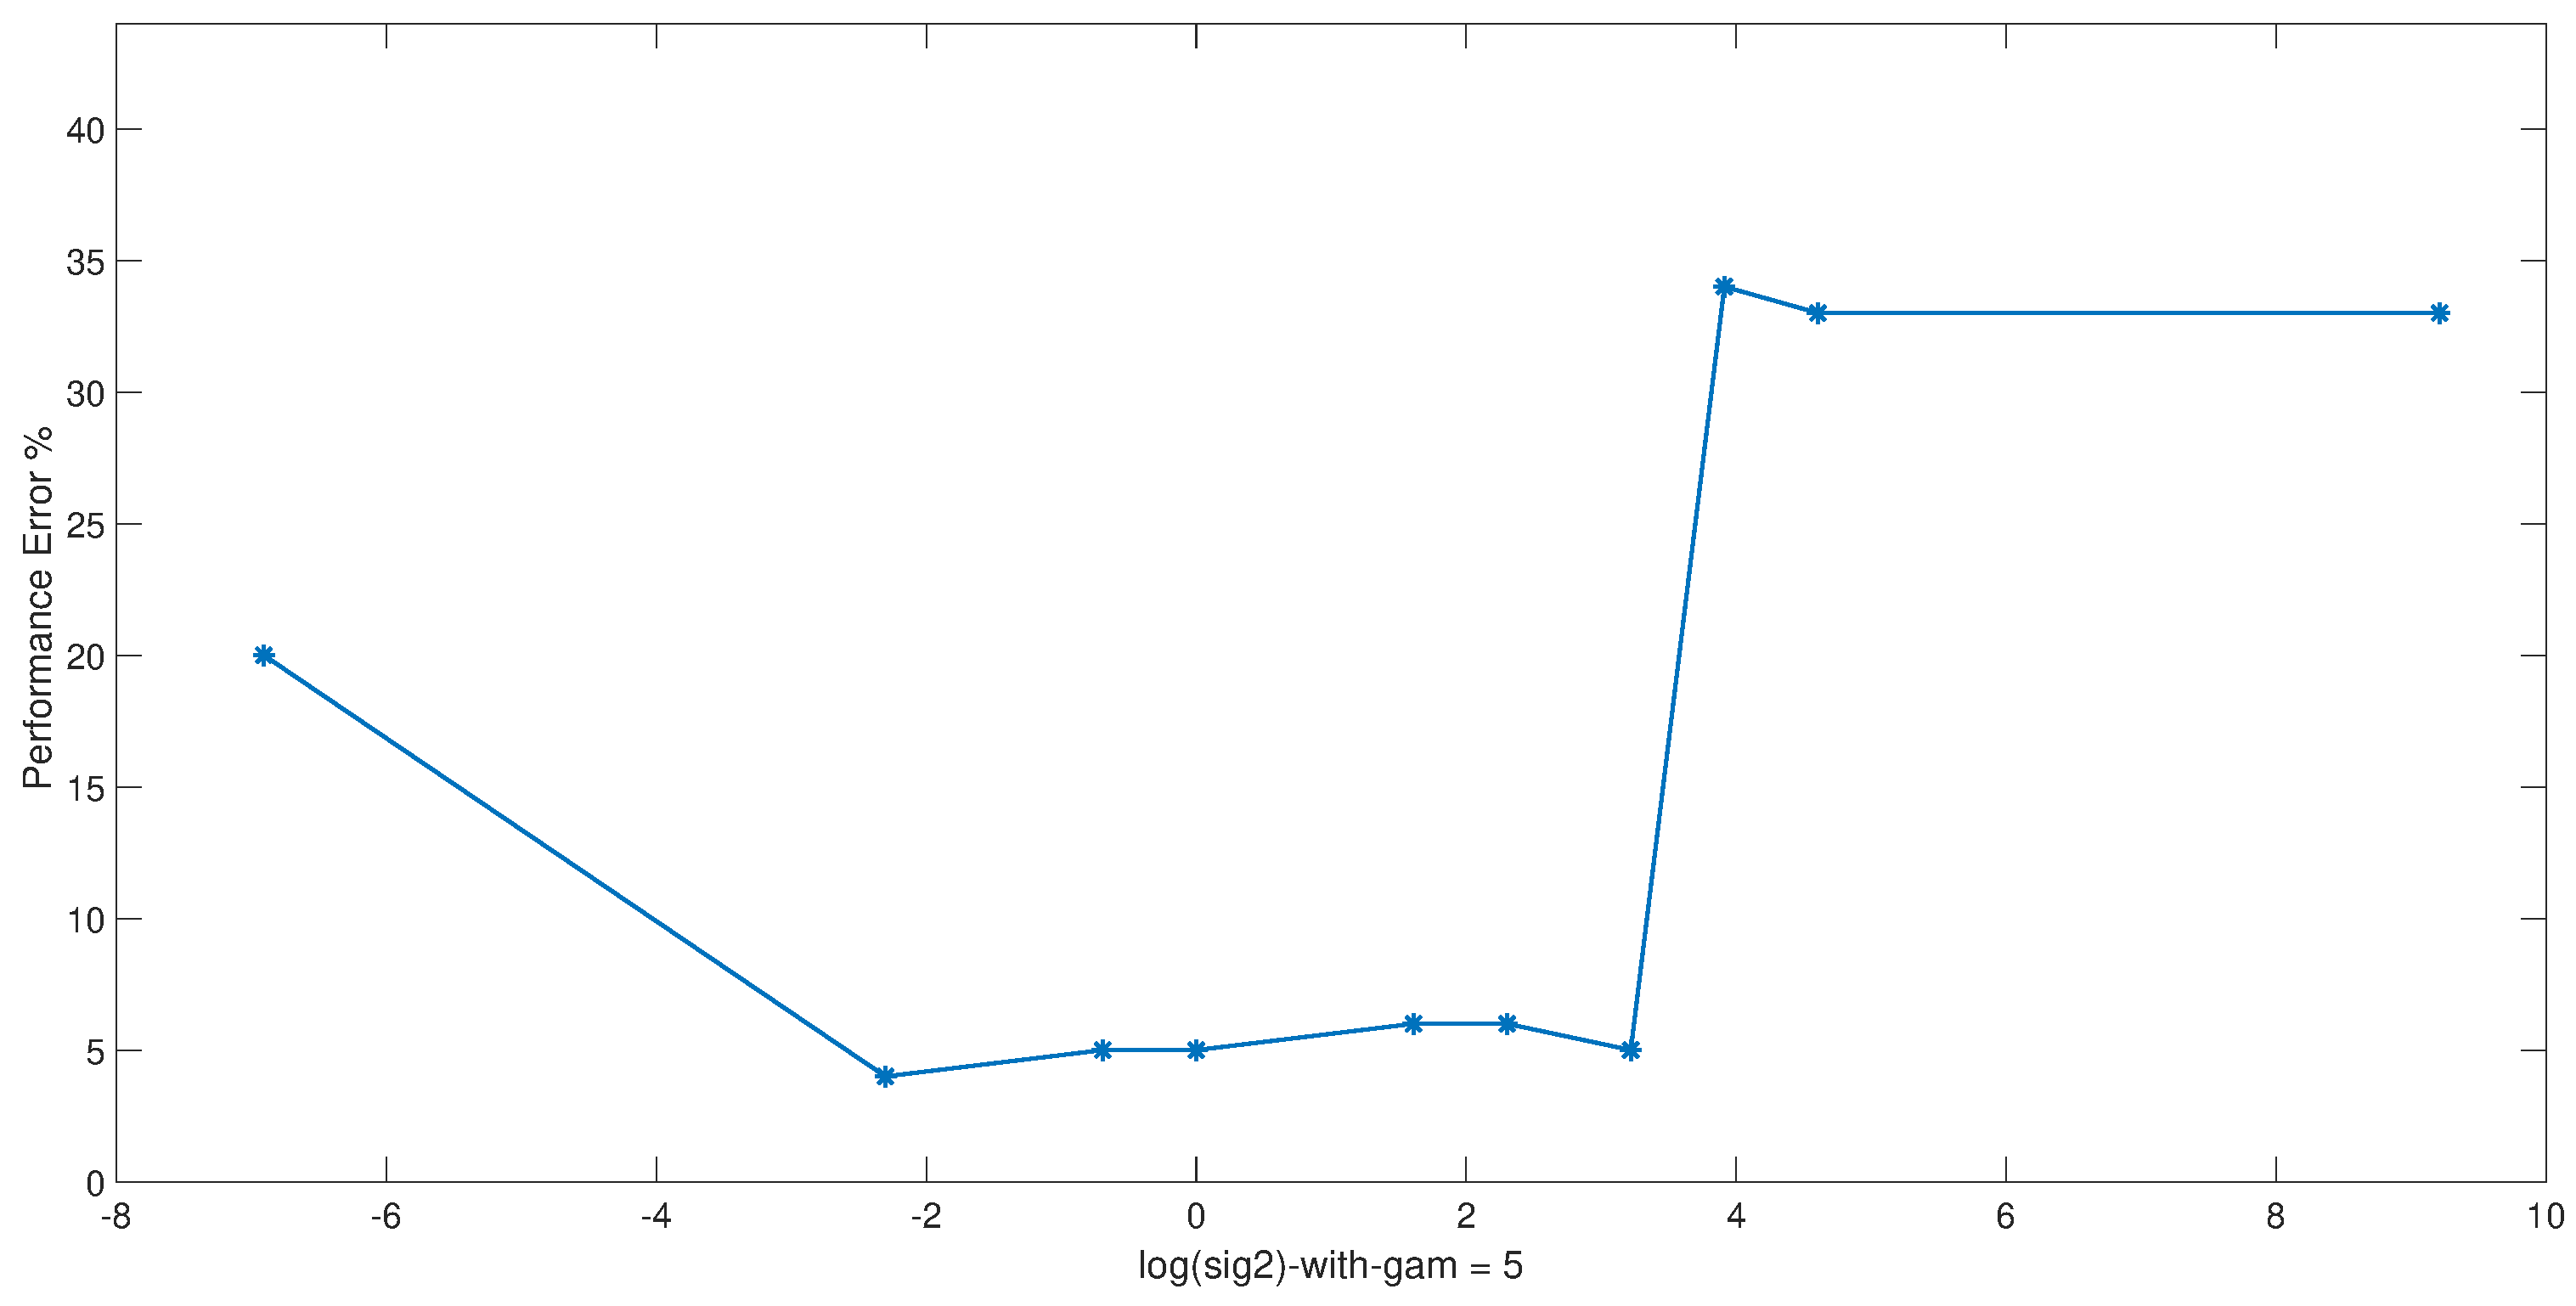
\includegraphics[height=0.35\linewidth,width=0.7\linewidth]{Exercise1/Report/Ex1.3_kCV_gam(5).eps}
				\caption{$\gamma$ = 5}
				\label{fig:kCV_gamma(5)}
			\end{subfigure}%
			\begin{subfigure}{.3\textwidth}
				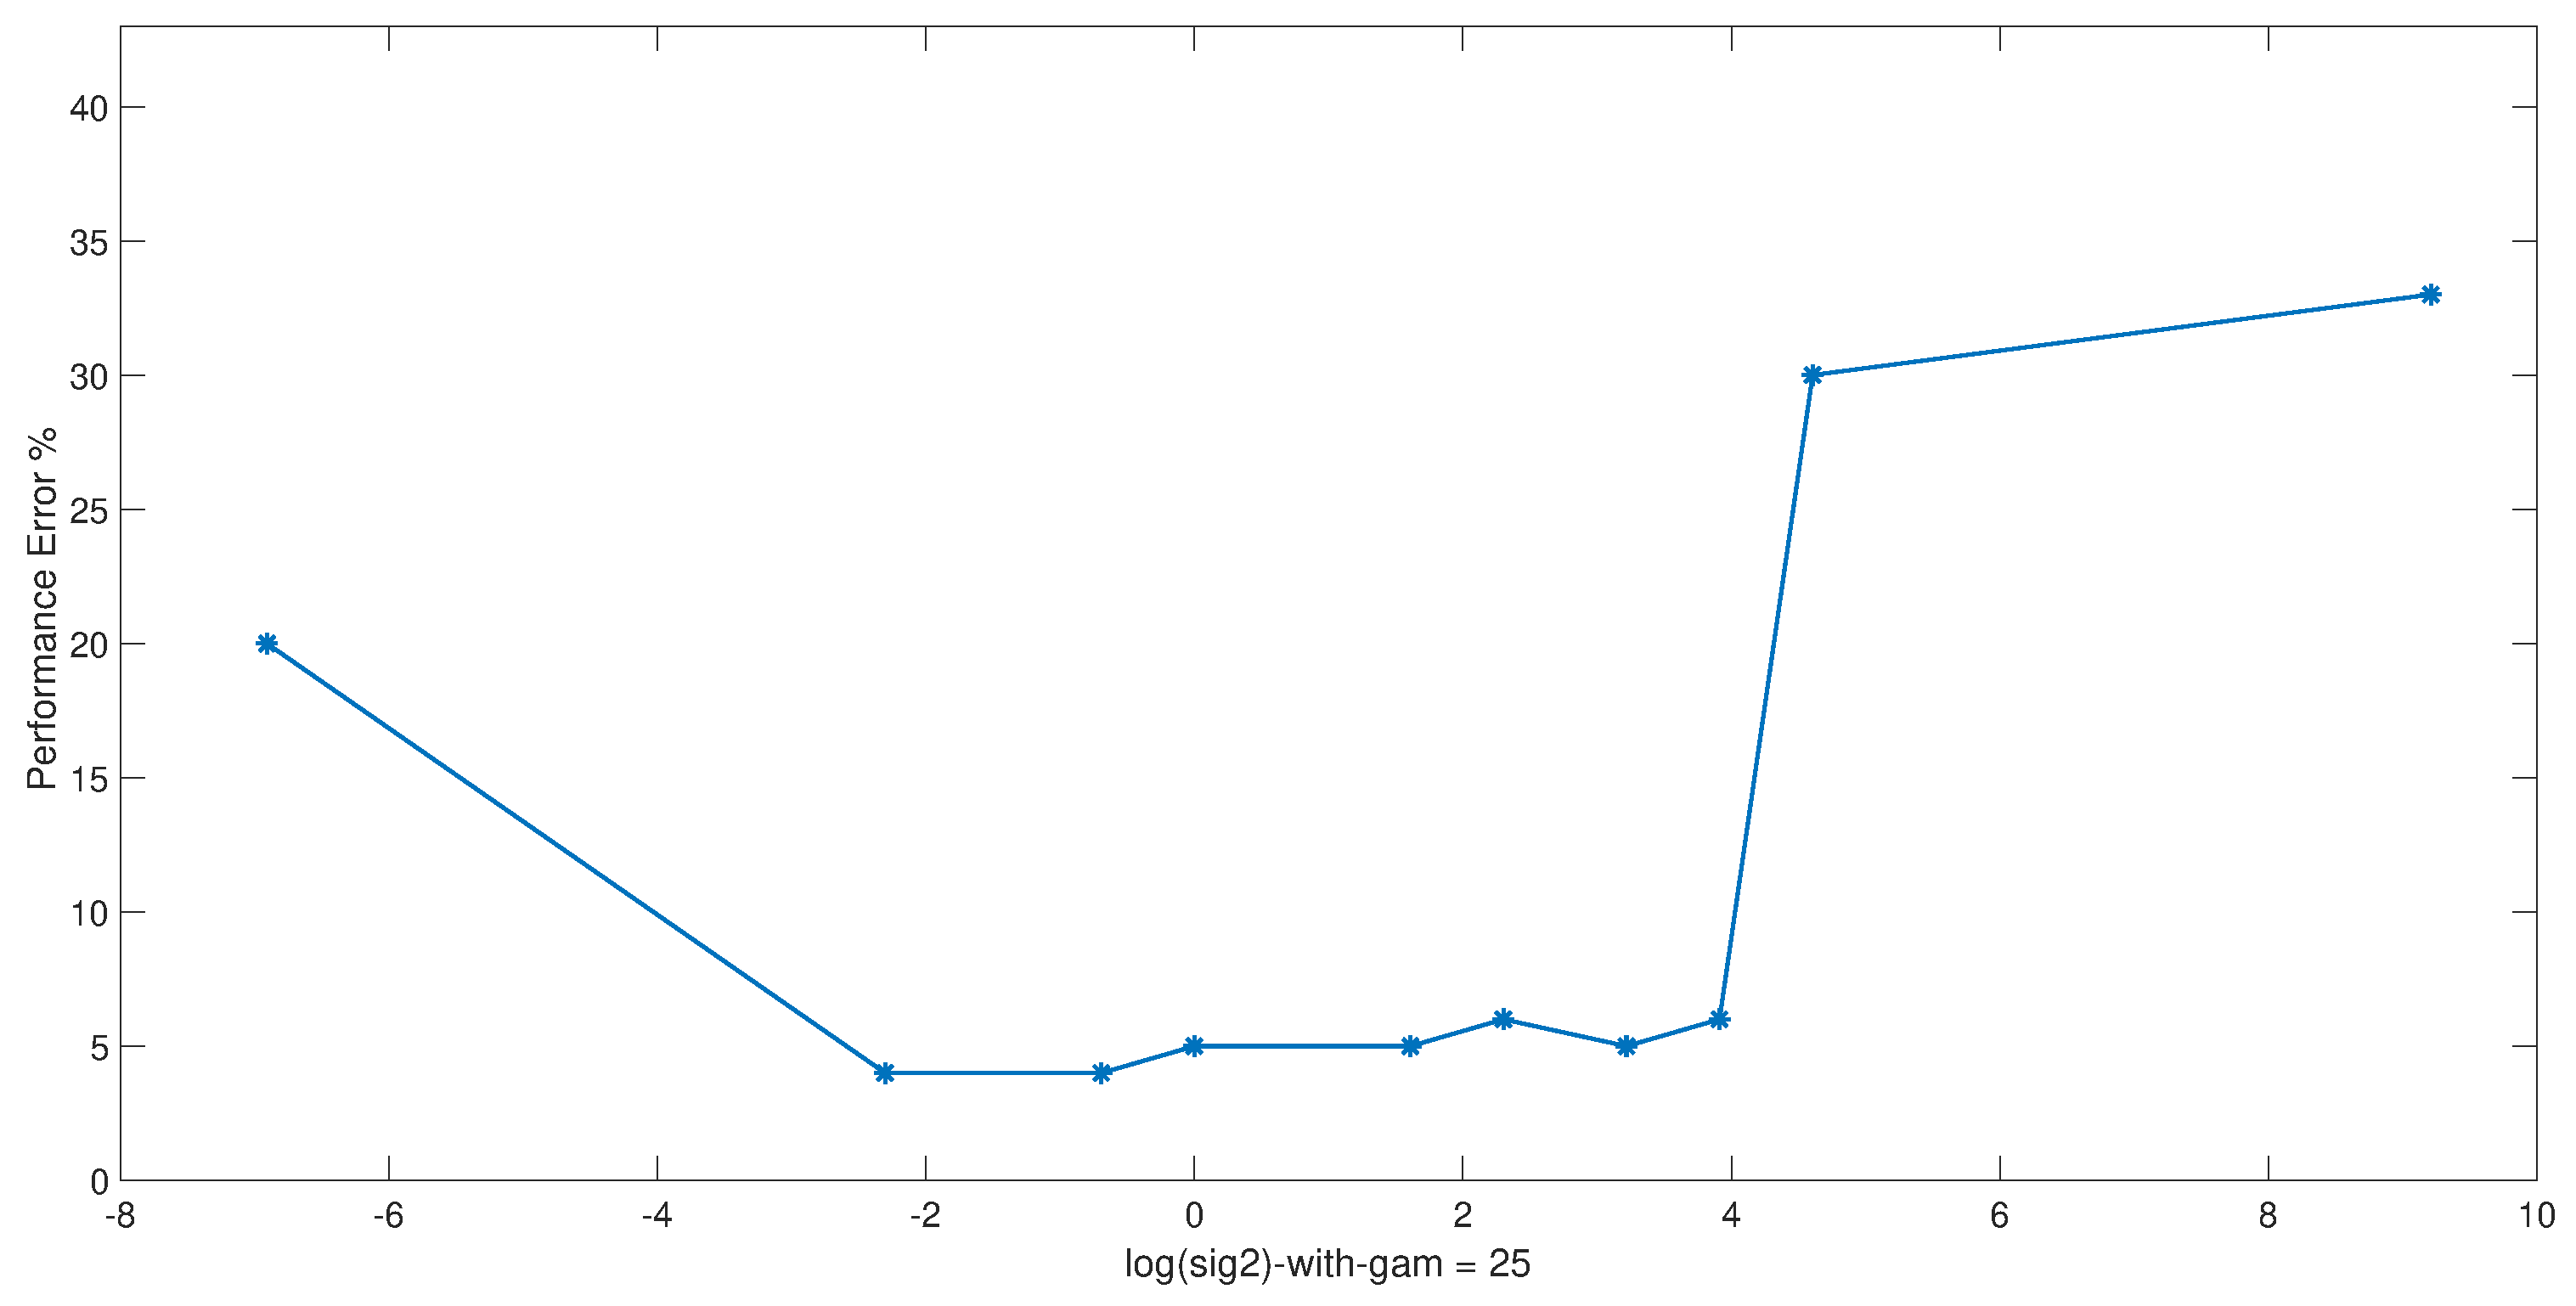
\includegraphics[height=0.35\linewidth,width=0.7\linewidth]{Exercise1/Report/Ex1.3_kCV_gam(25).eps}
				\caption{$\gamma$ = 25}
				\label{fig:kCV_gamma(25)}
			\end{subfigure}
			\begin{subfigure}{.3\textwidth}
				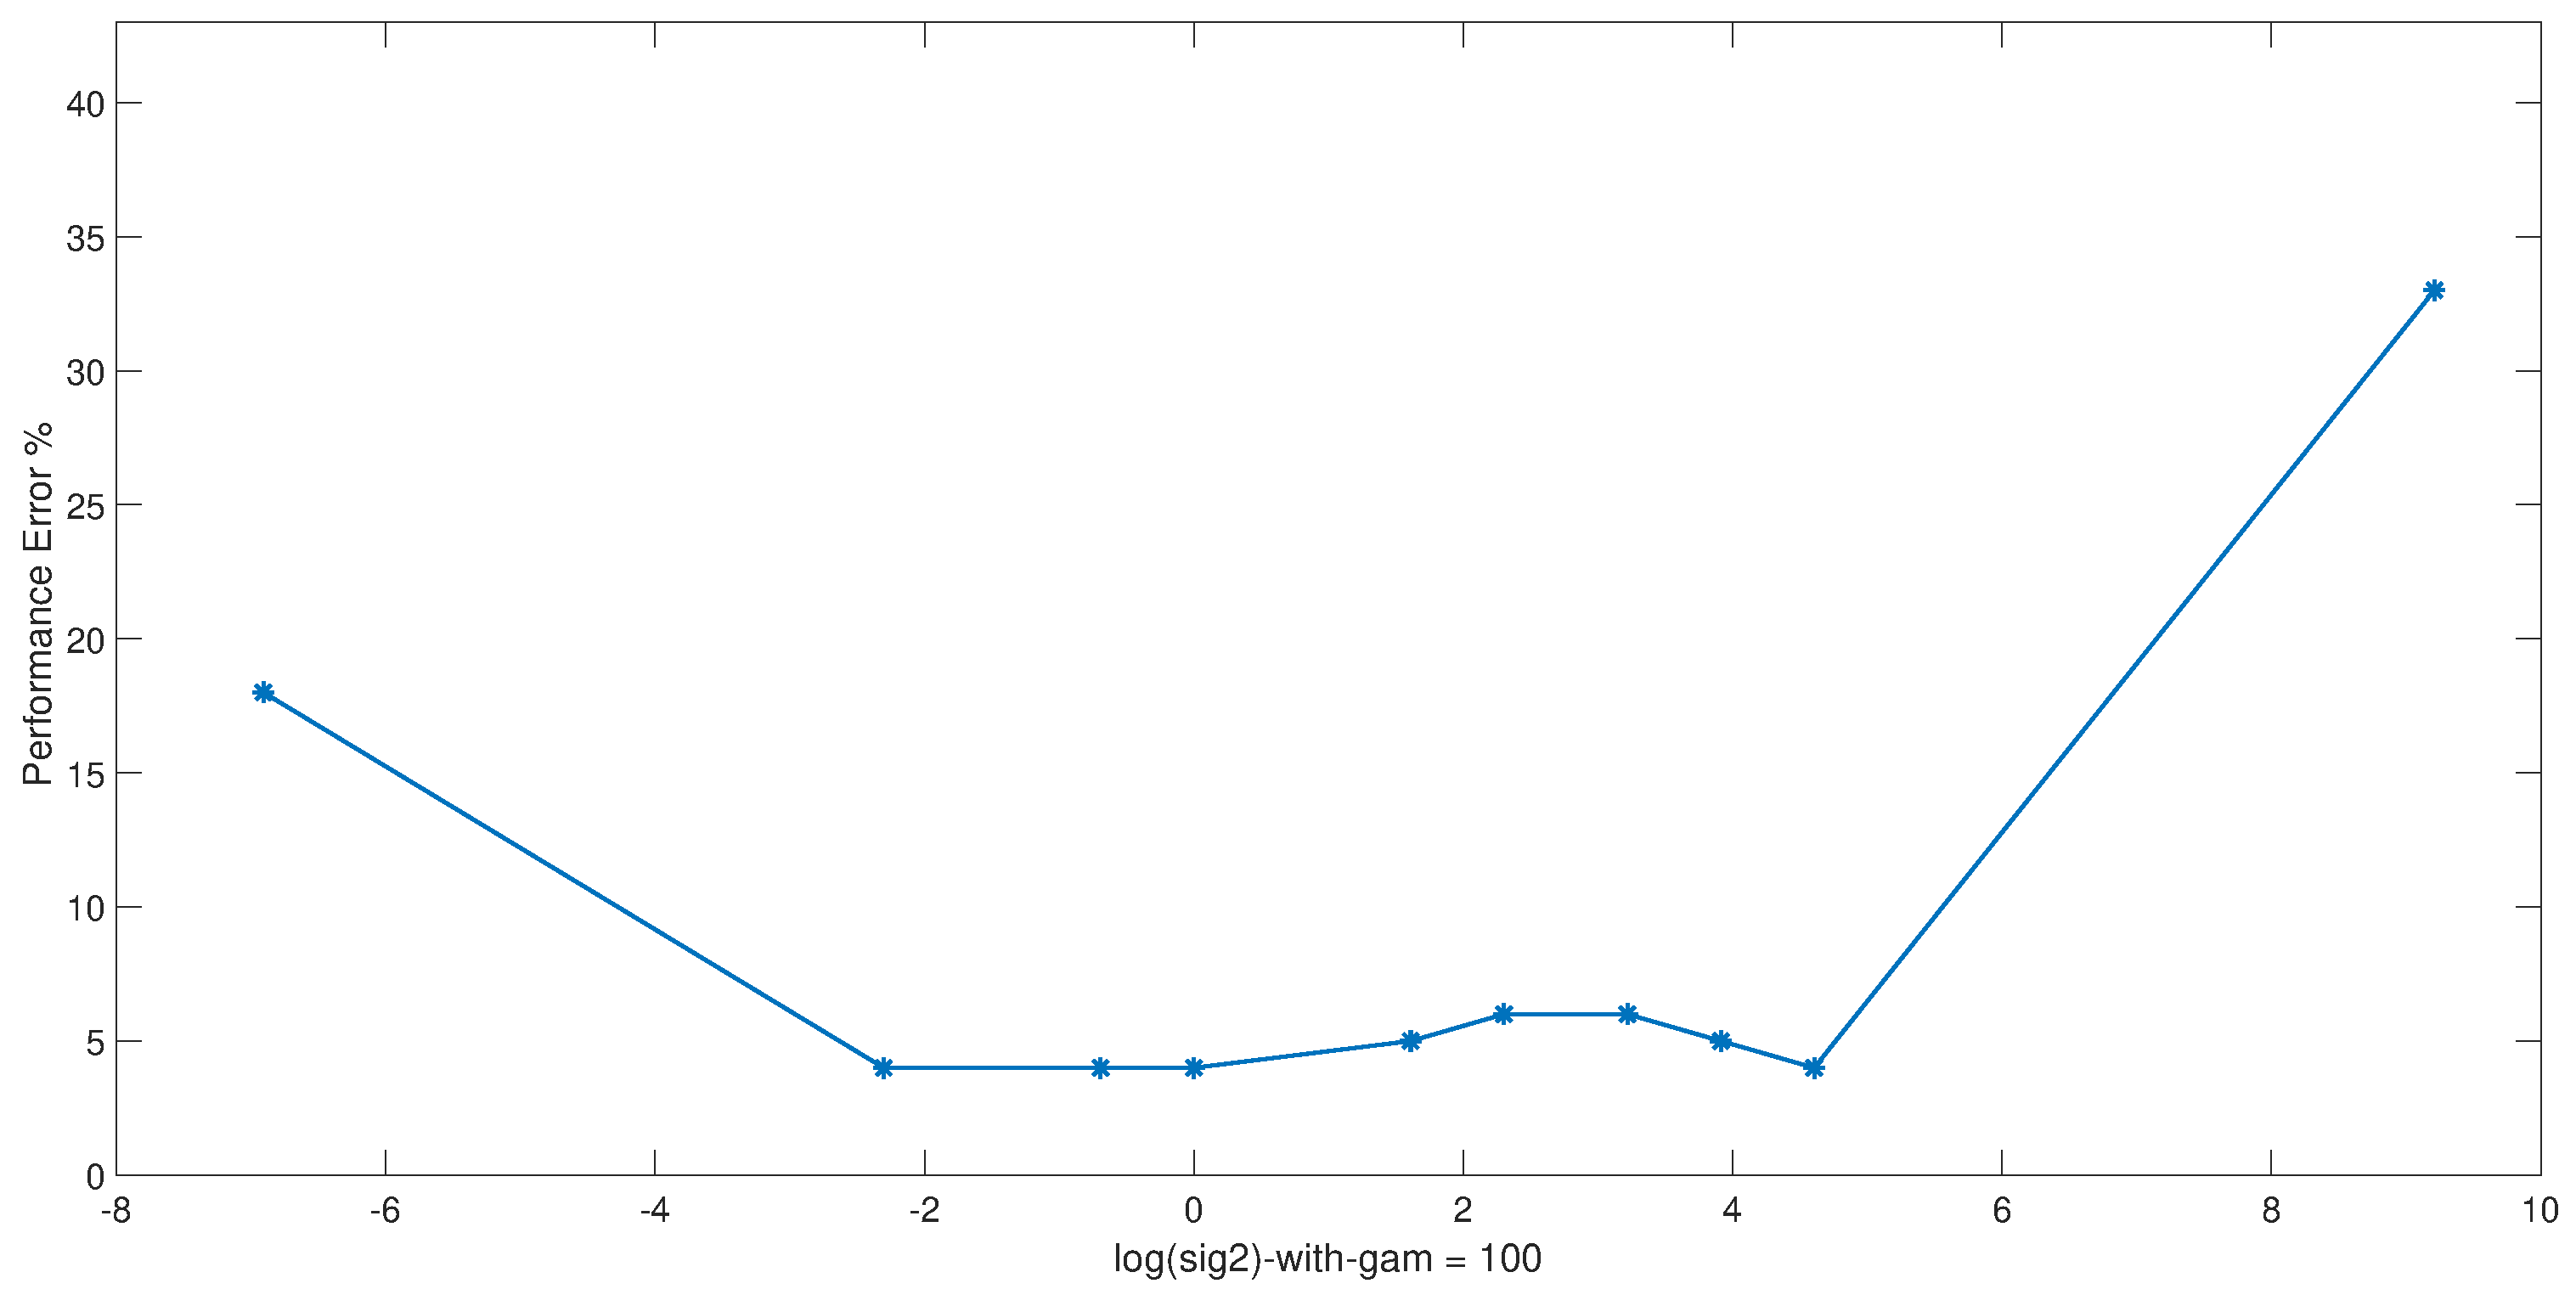
\includegraphics[height=0.35\linewidth,width=0.7\linewidth]{Exercise1/Report/Ex1.3_kCV_gam(100).eps}
				\caption{$\gamma$ = 100}
				\label{fig:kCV_gamma(100)}
			\end{subfigure}%
			\begin{subfigure}{.3\textwidth}
				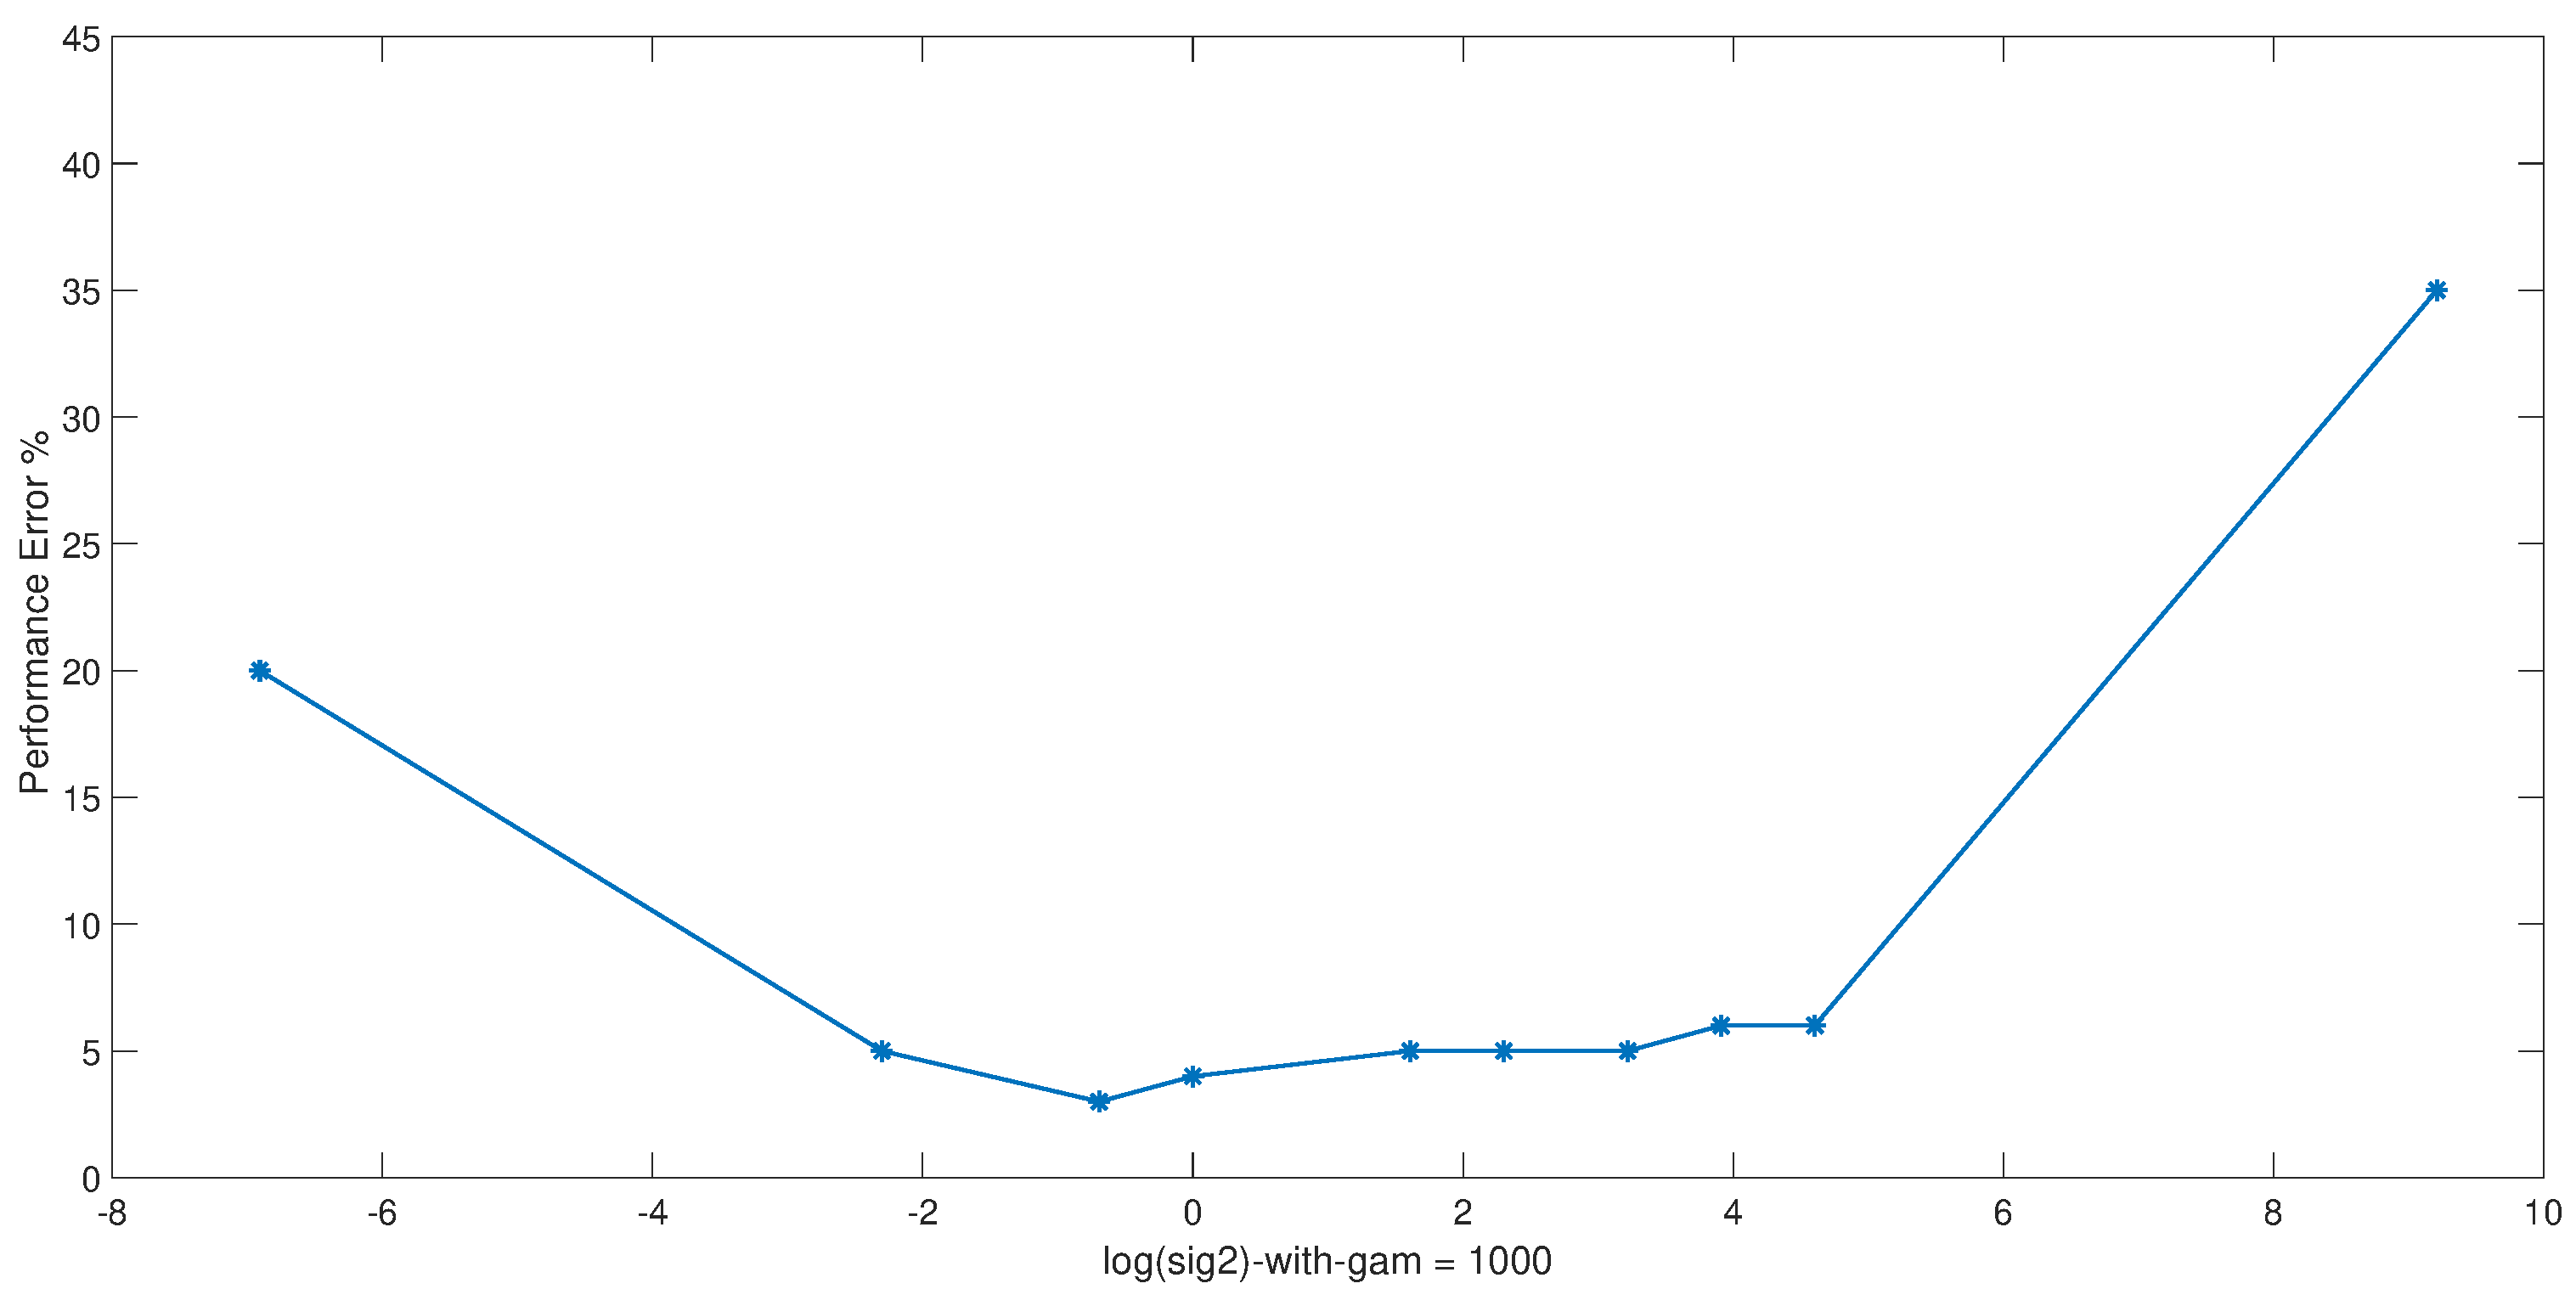
\includegraphics[height=0.35\linewidth,width=0.7\linewidth]{Exercise1/Report/Ex1.3_kCV_gam(1000).eps}
				\caption{$\gamma$ = 1000}
				\label{fig:kCV_gamma(1000)}
			\end{subfigure}%			
		}{%
			\caption{Iris data : k-fold CV (log($\sigma^2$) values for each level of $\gamma$ Vs Performance Error)  (\%)}\label{fig:kCV_gam}
		}
	\end{floatrow}
\end{figure}
The training data in k-fold cross validation is split into k subsets. Using $k-1$ sets from the $k$ subsets the model is trained and the validated using the $k^{th}$ set. This is repeated over all the k subsets of data in a loop. Next we perform leave-one-out method similar to k-fold cross validation. The result of these methods is not performance rate but rather a average of errors over number of iterations of k-sets. The model performance is shown in figures \ref{fig:kCV_gam} and \ref{fig:loo_gam}. It can be seen that the performance for both k-fold and leave-one-out methods are nearly same. Therefore, in case of larger data sets, k-fold method is preferred as it is computationally faster than leave-one-out and for smaller data sets leave-one-out is preferred. From figure \ref{fig:rand_3D}, it can be seen that random split validation method exhibits high variance compared to k-fold and leave-one-out methods in figures \ref{fig:kCV_3D} and \ref{fig:loo_3D} giving a clear indication of best (purple color) and least performing (pale yellow and cyan) $\gamma$ and $\sigma^2$ values.  This can also be seen from the smoothness of curves in the case of k-fold and leave-one-out.\\

\begin{wraptable}[4]{r}{.5\textwidth}
	\caption{Optimal ($\gamma$, $\sigma^2$) combinations}\label{table:4}
	\begin{tabular}{|c|c|}
		\hline
		$\gamma$ & $\sigma^2$ \\ \hline
		25 & (0.1, 0.5, 1, 5) \\ \hline
		100 & (0.1, 0.5, 1, 5)  \\ \hline
		1000 & (0.5, 1, 5)  \\ \hline
	\end{tabular}
\end{wraptable}
 The optimal values of ($\gamma$, $\sigma^2$) pair can be chosen from figures \ref{fig:kCV_gam} and \ref{fig:loo_gam} that gives the least performance error. Some good combinations of ($\gamma$, $\sigma^2$) can be as shown in table \ref{table:4}.\\
 \begin{figure}[!htbp]
	\begin{floatrow}
		\ffigbox{%
			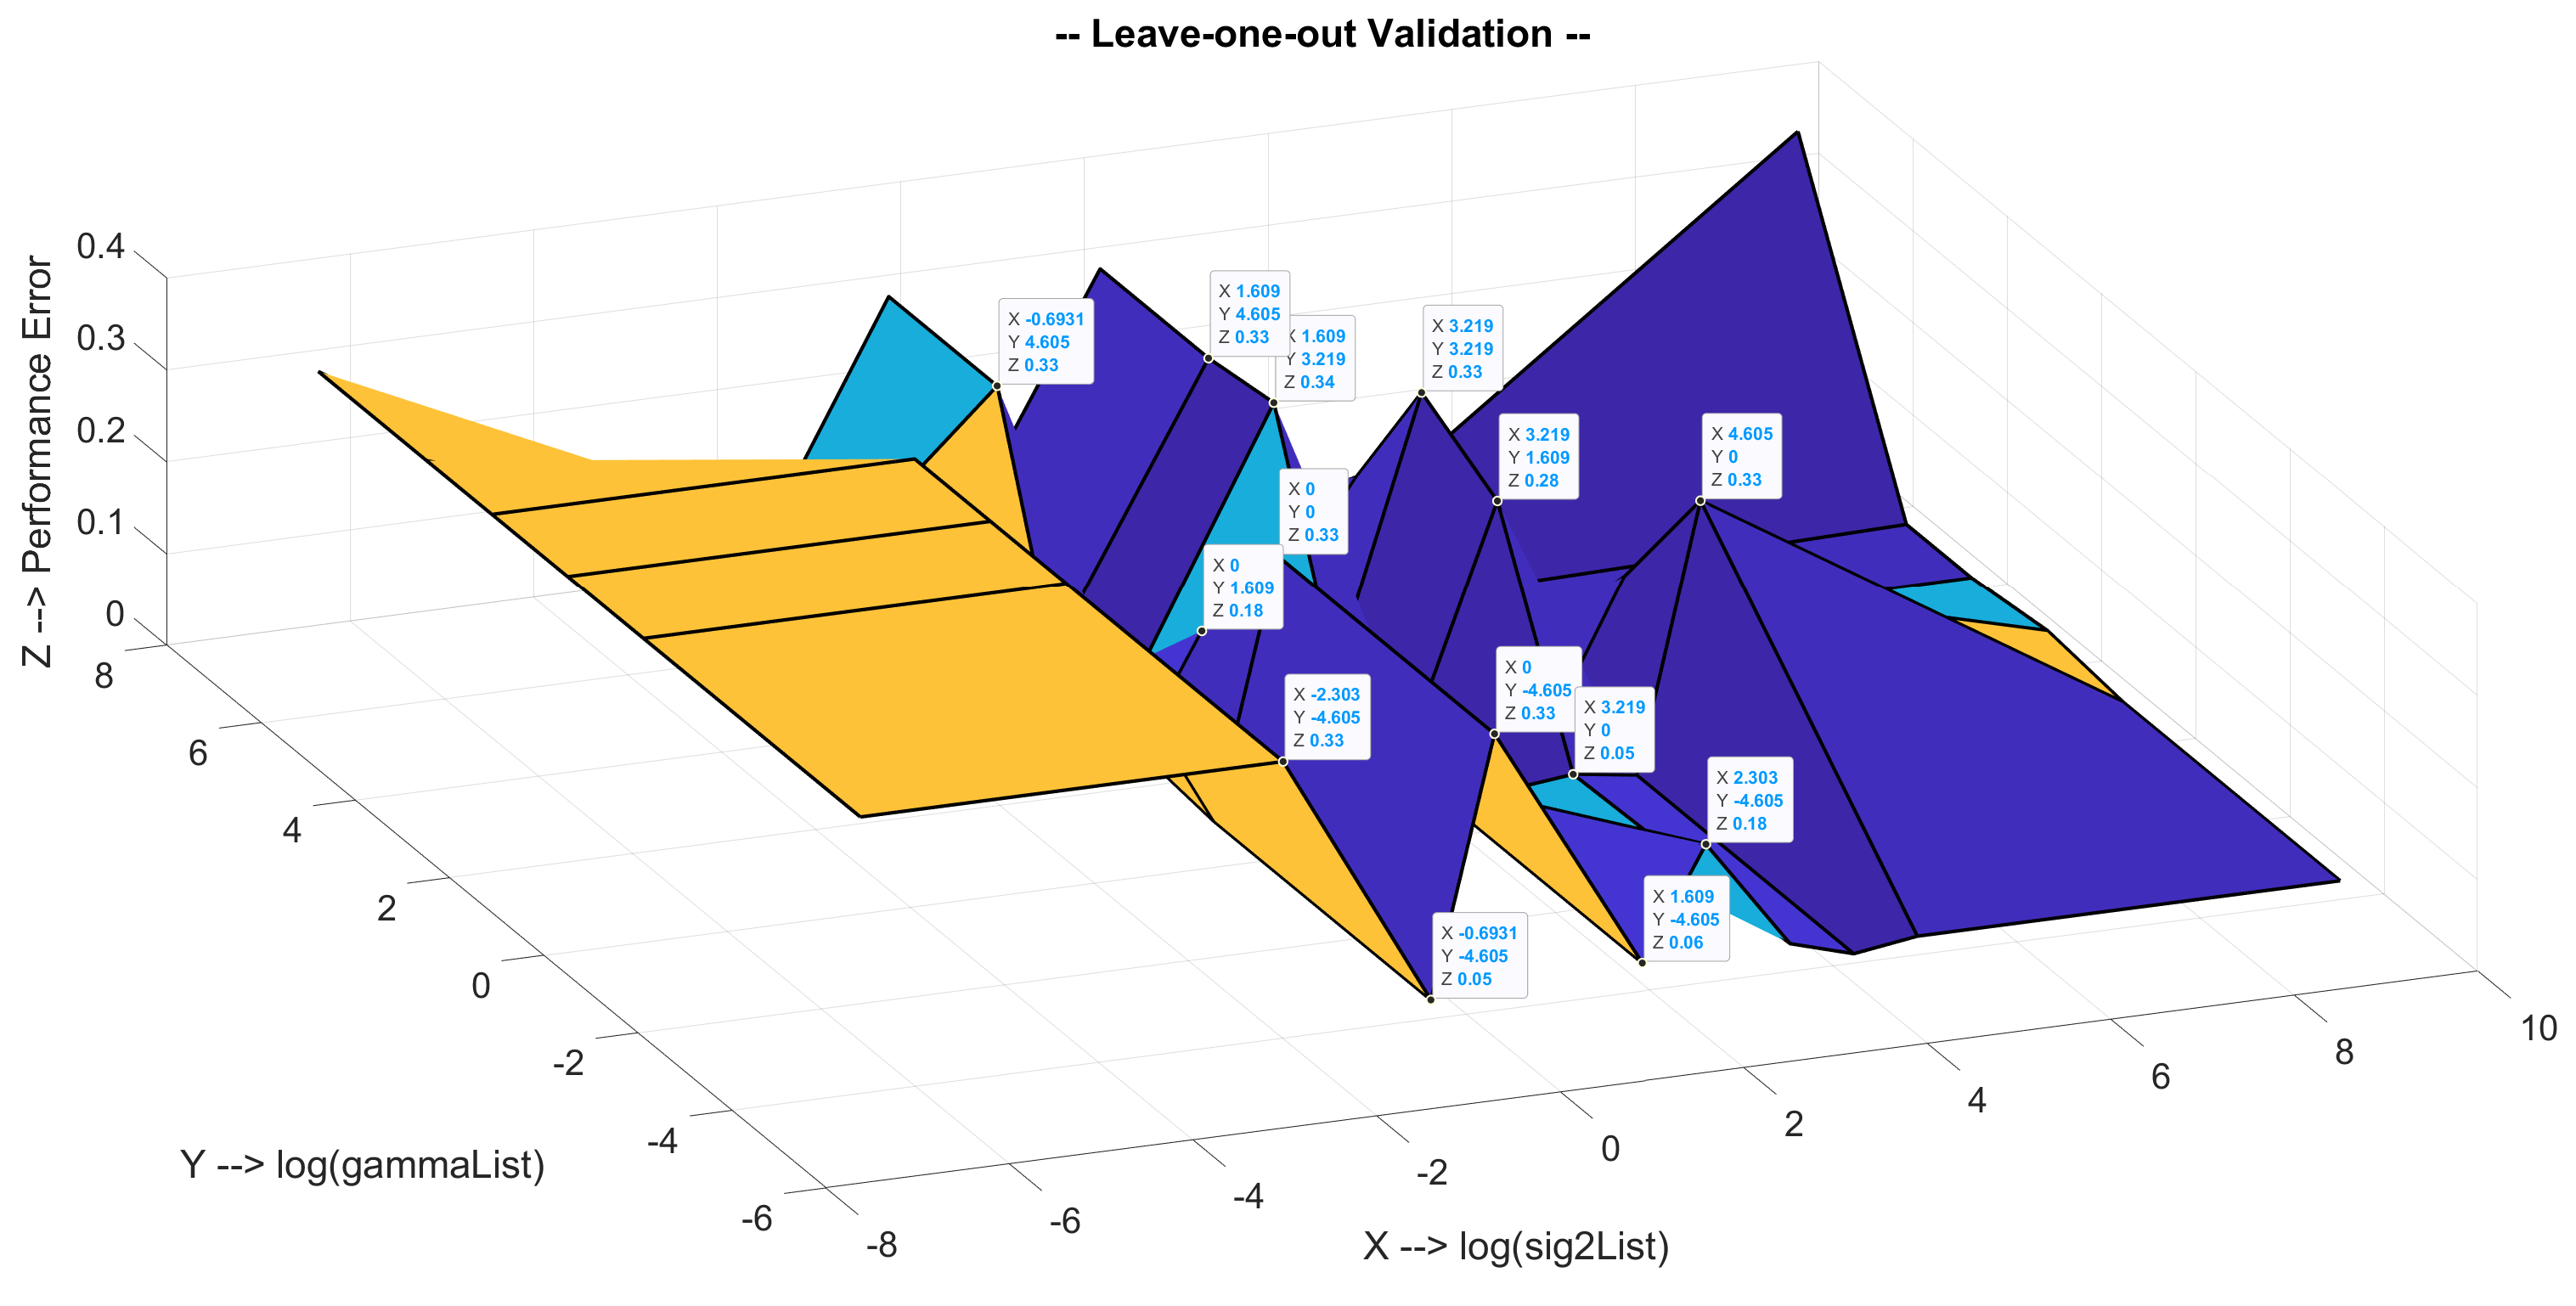
\includegraphics[height=0.75\linewidth,width= 0.8\linewidth]{Exercise1/Report/Ex1.3_loo_surf.eps} %
		}{%
			\caption{Leave-one-out Validation - (log($\sigma^2$) vs log
				($\gamma$) vs Performane Error)}\label{fig:loo_3D}%
		}
		\ffigbox{%
			\begin{subfigure}{.3\textwidth}
				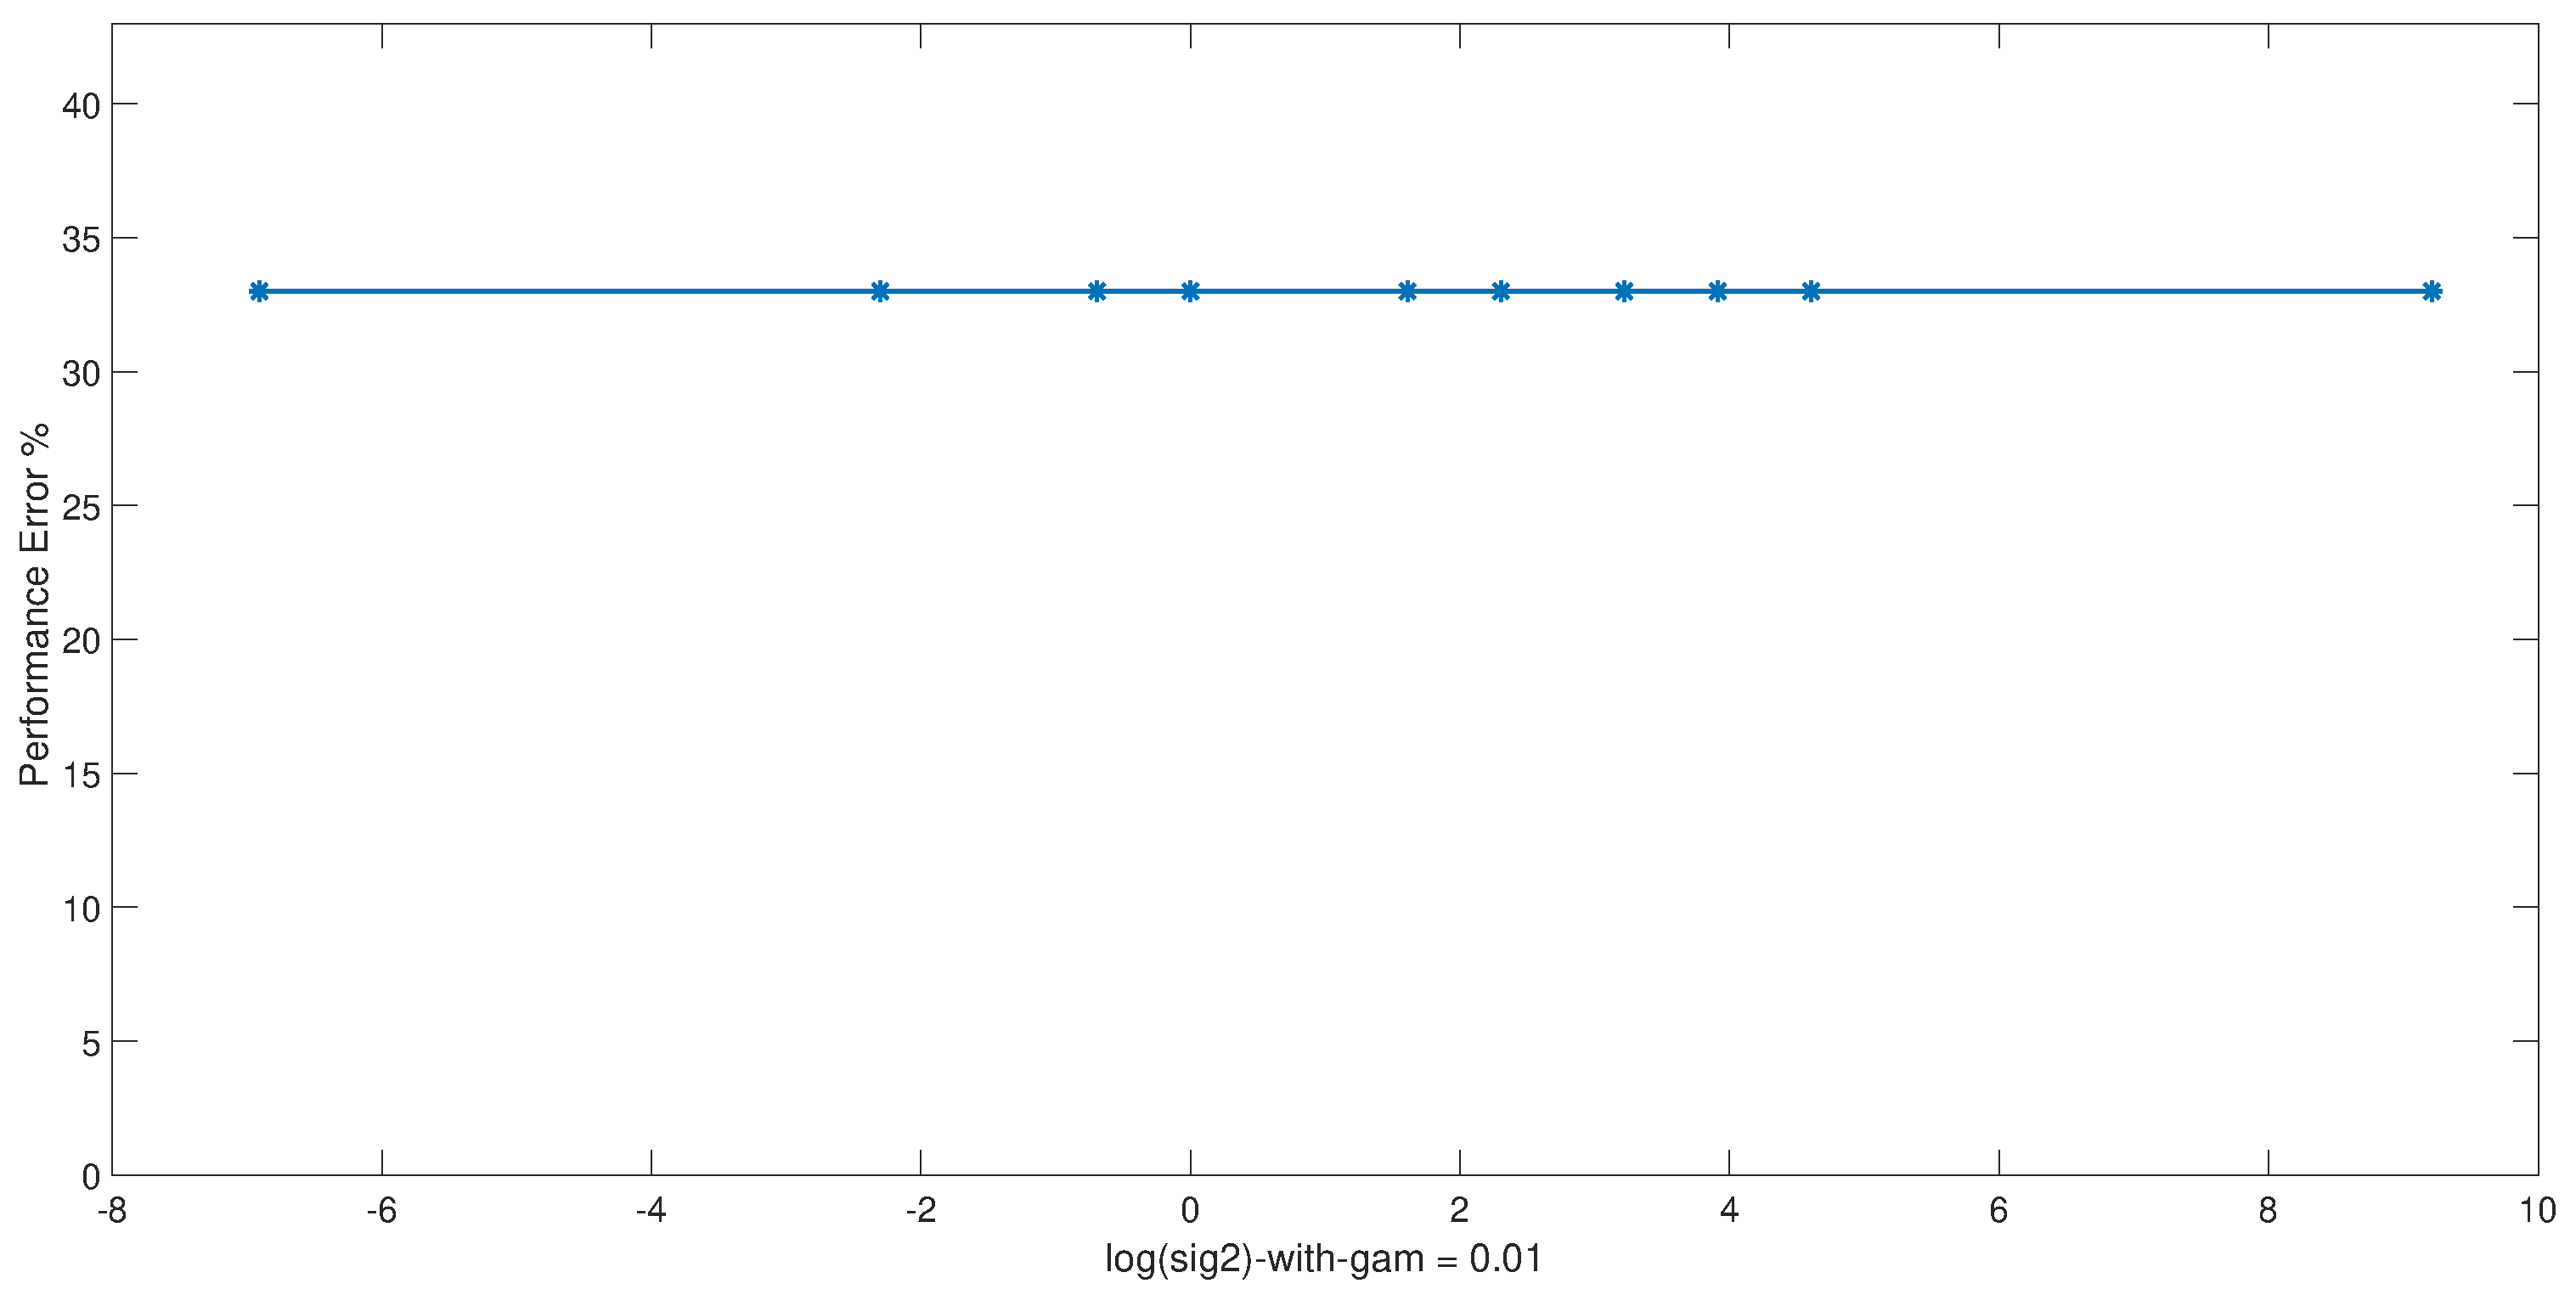
\includegraphics[height=0.35\linewidth,width=0.7\linewidth]{Exercise1/Report/Ex1.3_loo_gam(0.01).eps}
				\caption{$\gamma$ = 0.01}
				\label{fig:loo_gamma(0.01)}
			\end{subfigure}%
			\begin{subfigure}{.3\textwidth}
				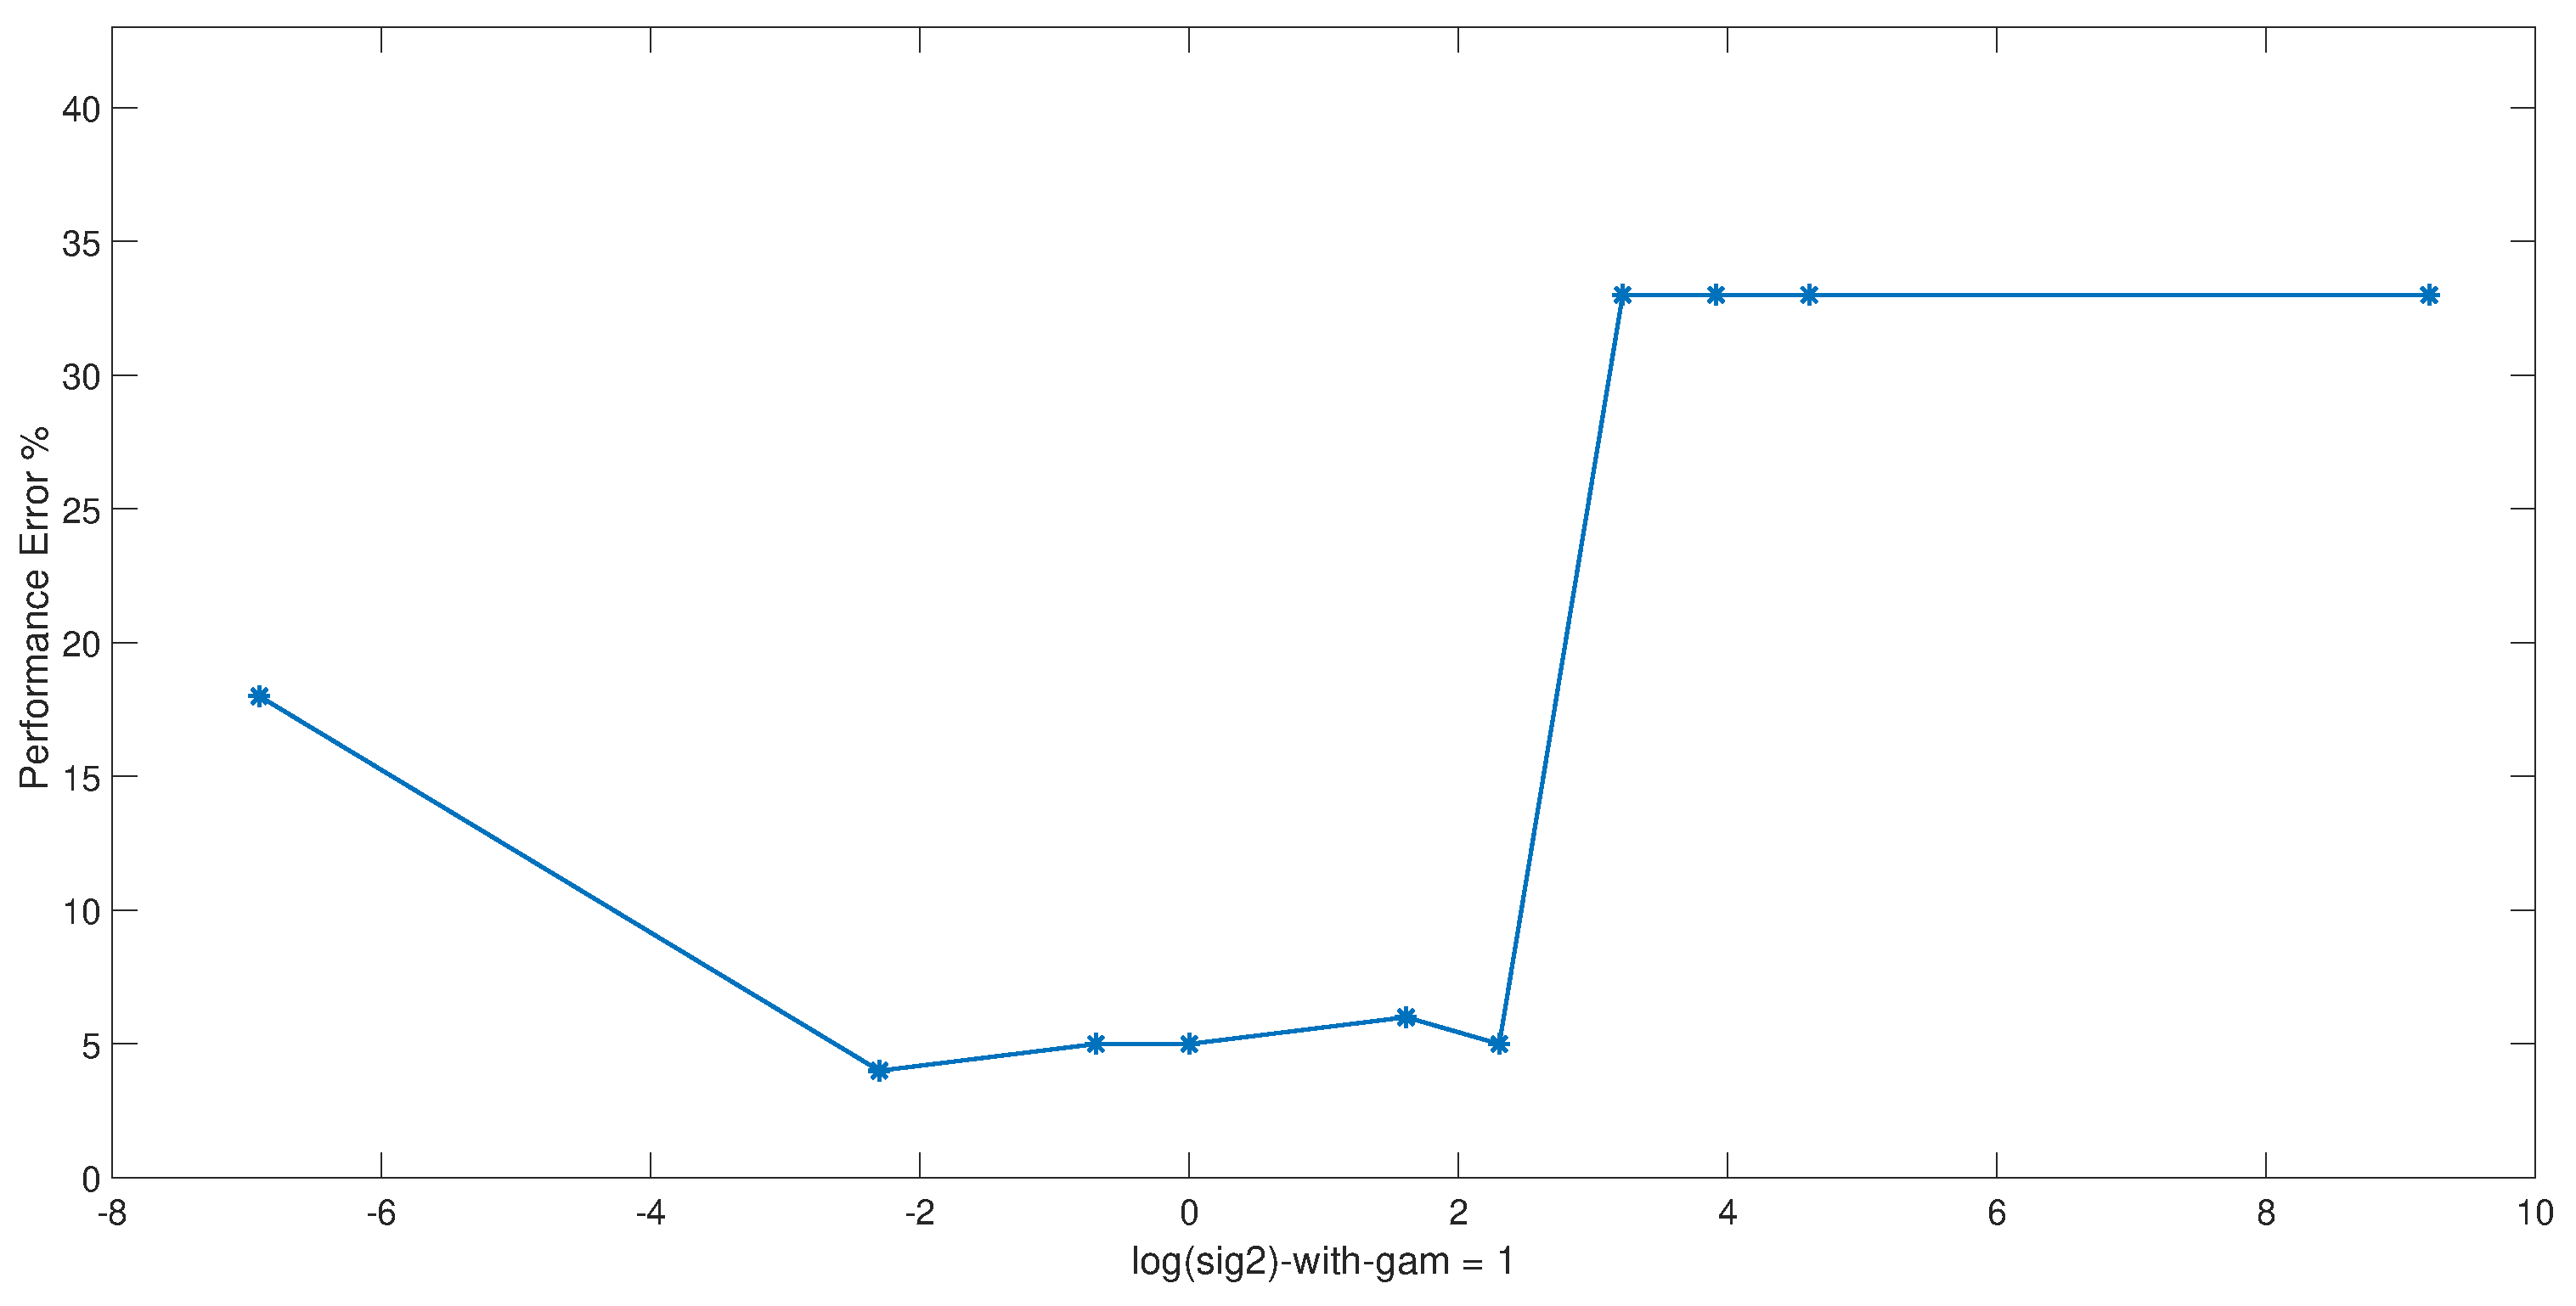
\includegraphics[height=0.35\linewidth,width=0.7\linewidth]{Exercise1/Report/Ex1.3_loo_gam(1).eps}
				\caption{$\gamma$ = 1}
				\label{fig:loo_gamma(1))}
			\end{subfigure}
			\begin{subfigure}{.3\textwidth}
				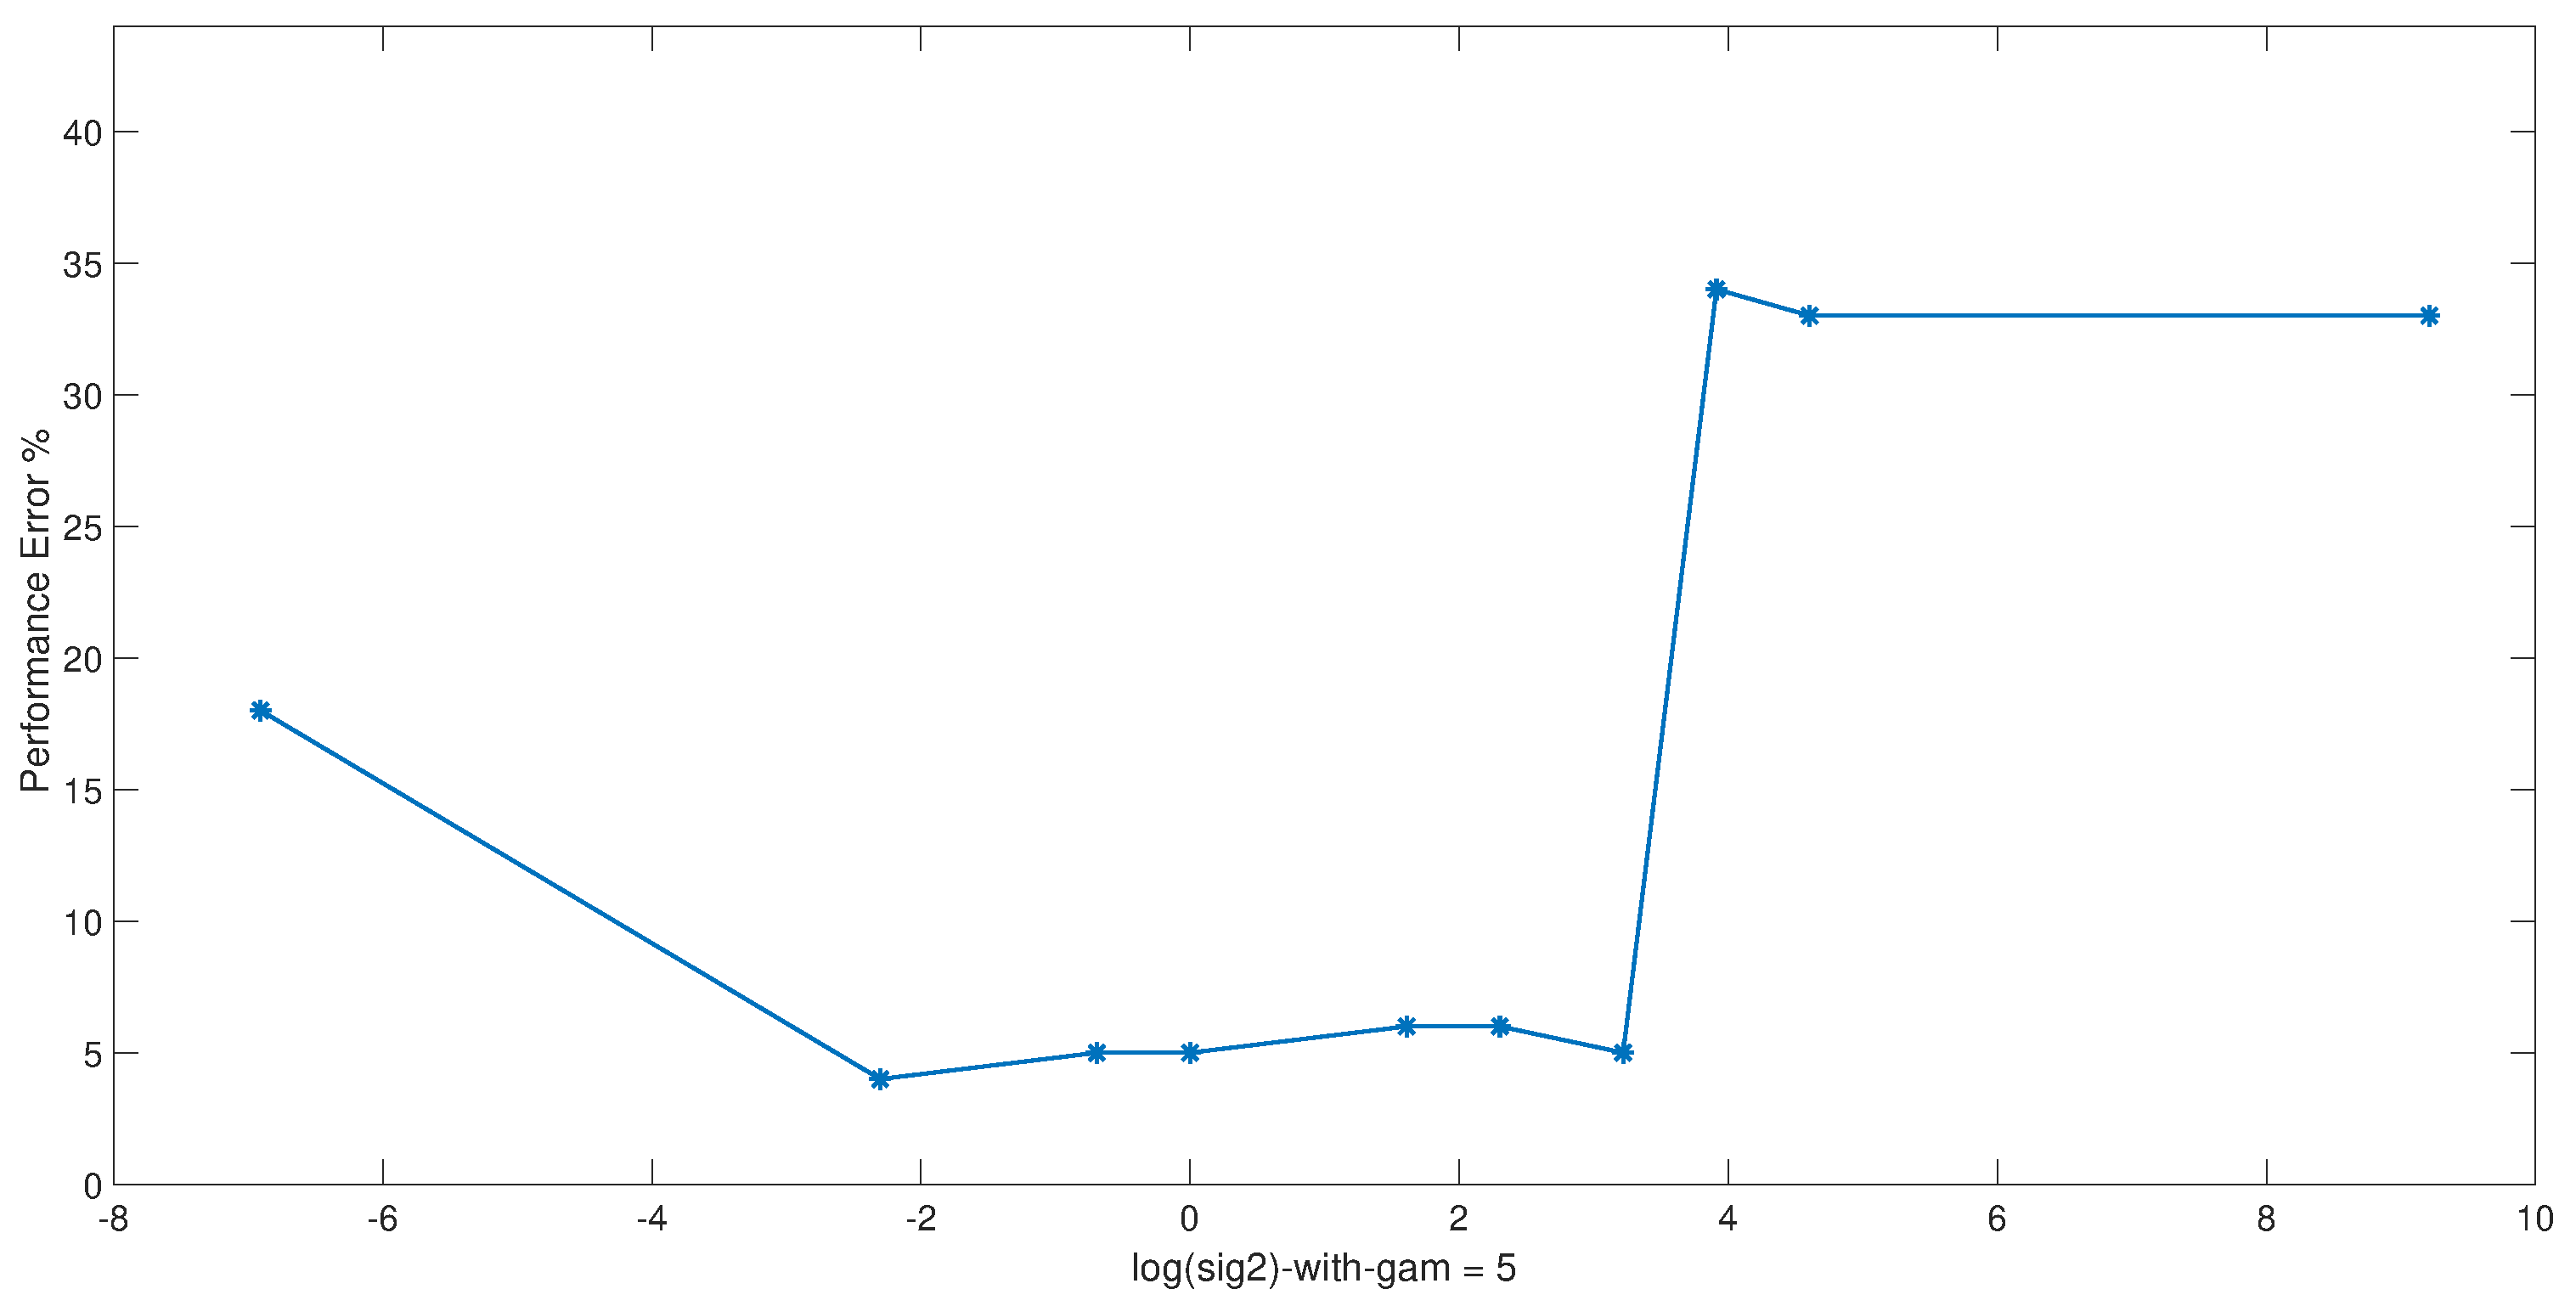
\includegraphics[height=0.35\linewidth,width=0.7\linewidth]{Exercise1/Report/Ex1.3_loo_gam(5).eps}
				\caption{$\gamma$ = 5}
				\label{fig:loo_gamma(5)}
			\end{subfigure}%
			\begin{subfigure}{.3\textwidth}
				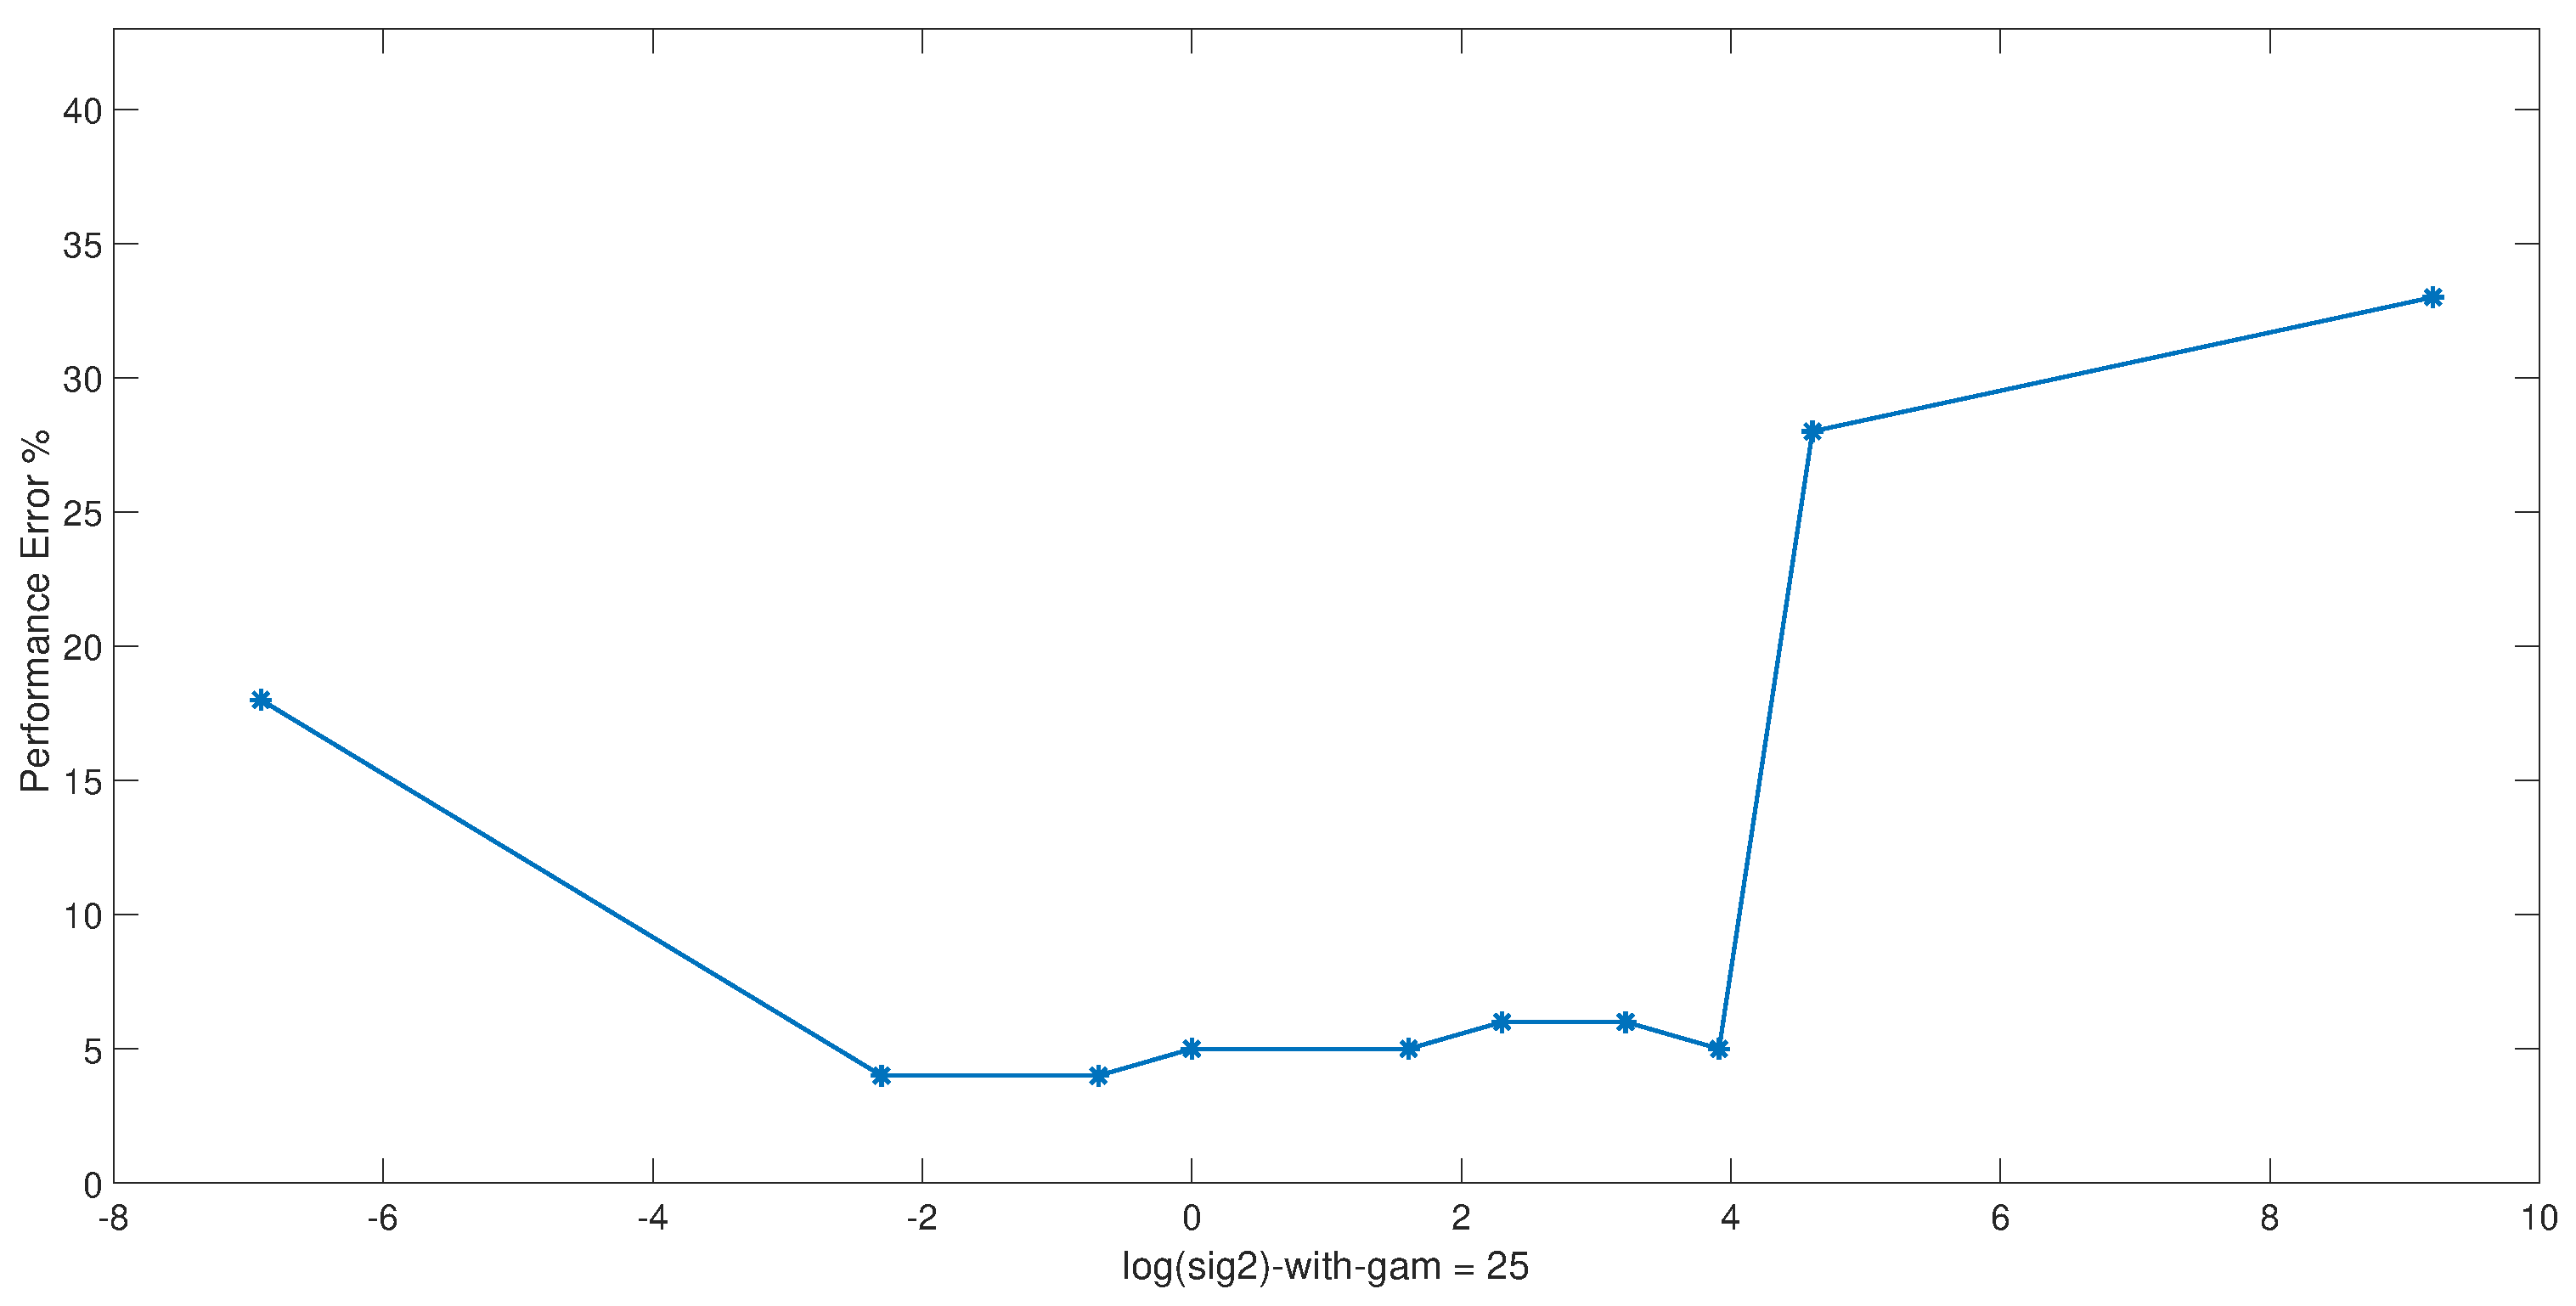
\includegraphics[height=0.35\linewidth,width=0.7\linewidth]{Exercise1/Report/Ex1.3_loo_gam(25).eps}
				\caption{$\gamma$ = 25}
				\label{fig:loo_gamma(25)}
			\end{subfigure}
			\begin{subfigure}{.3\textwidth}
				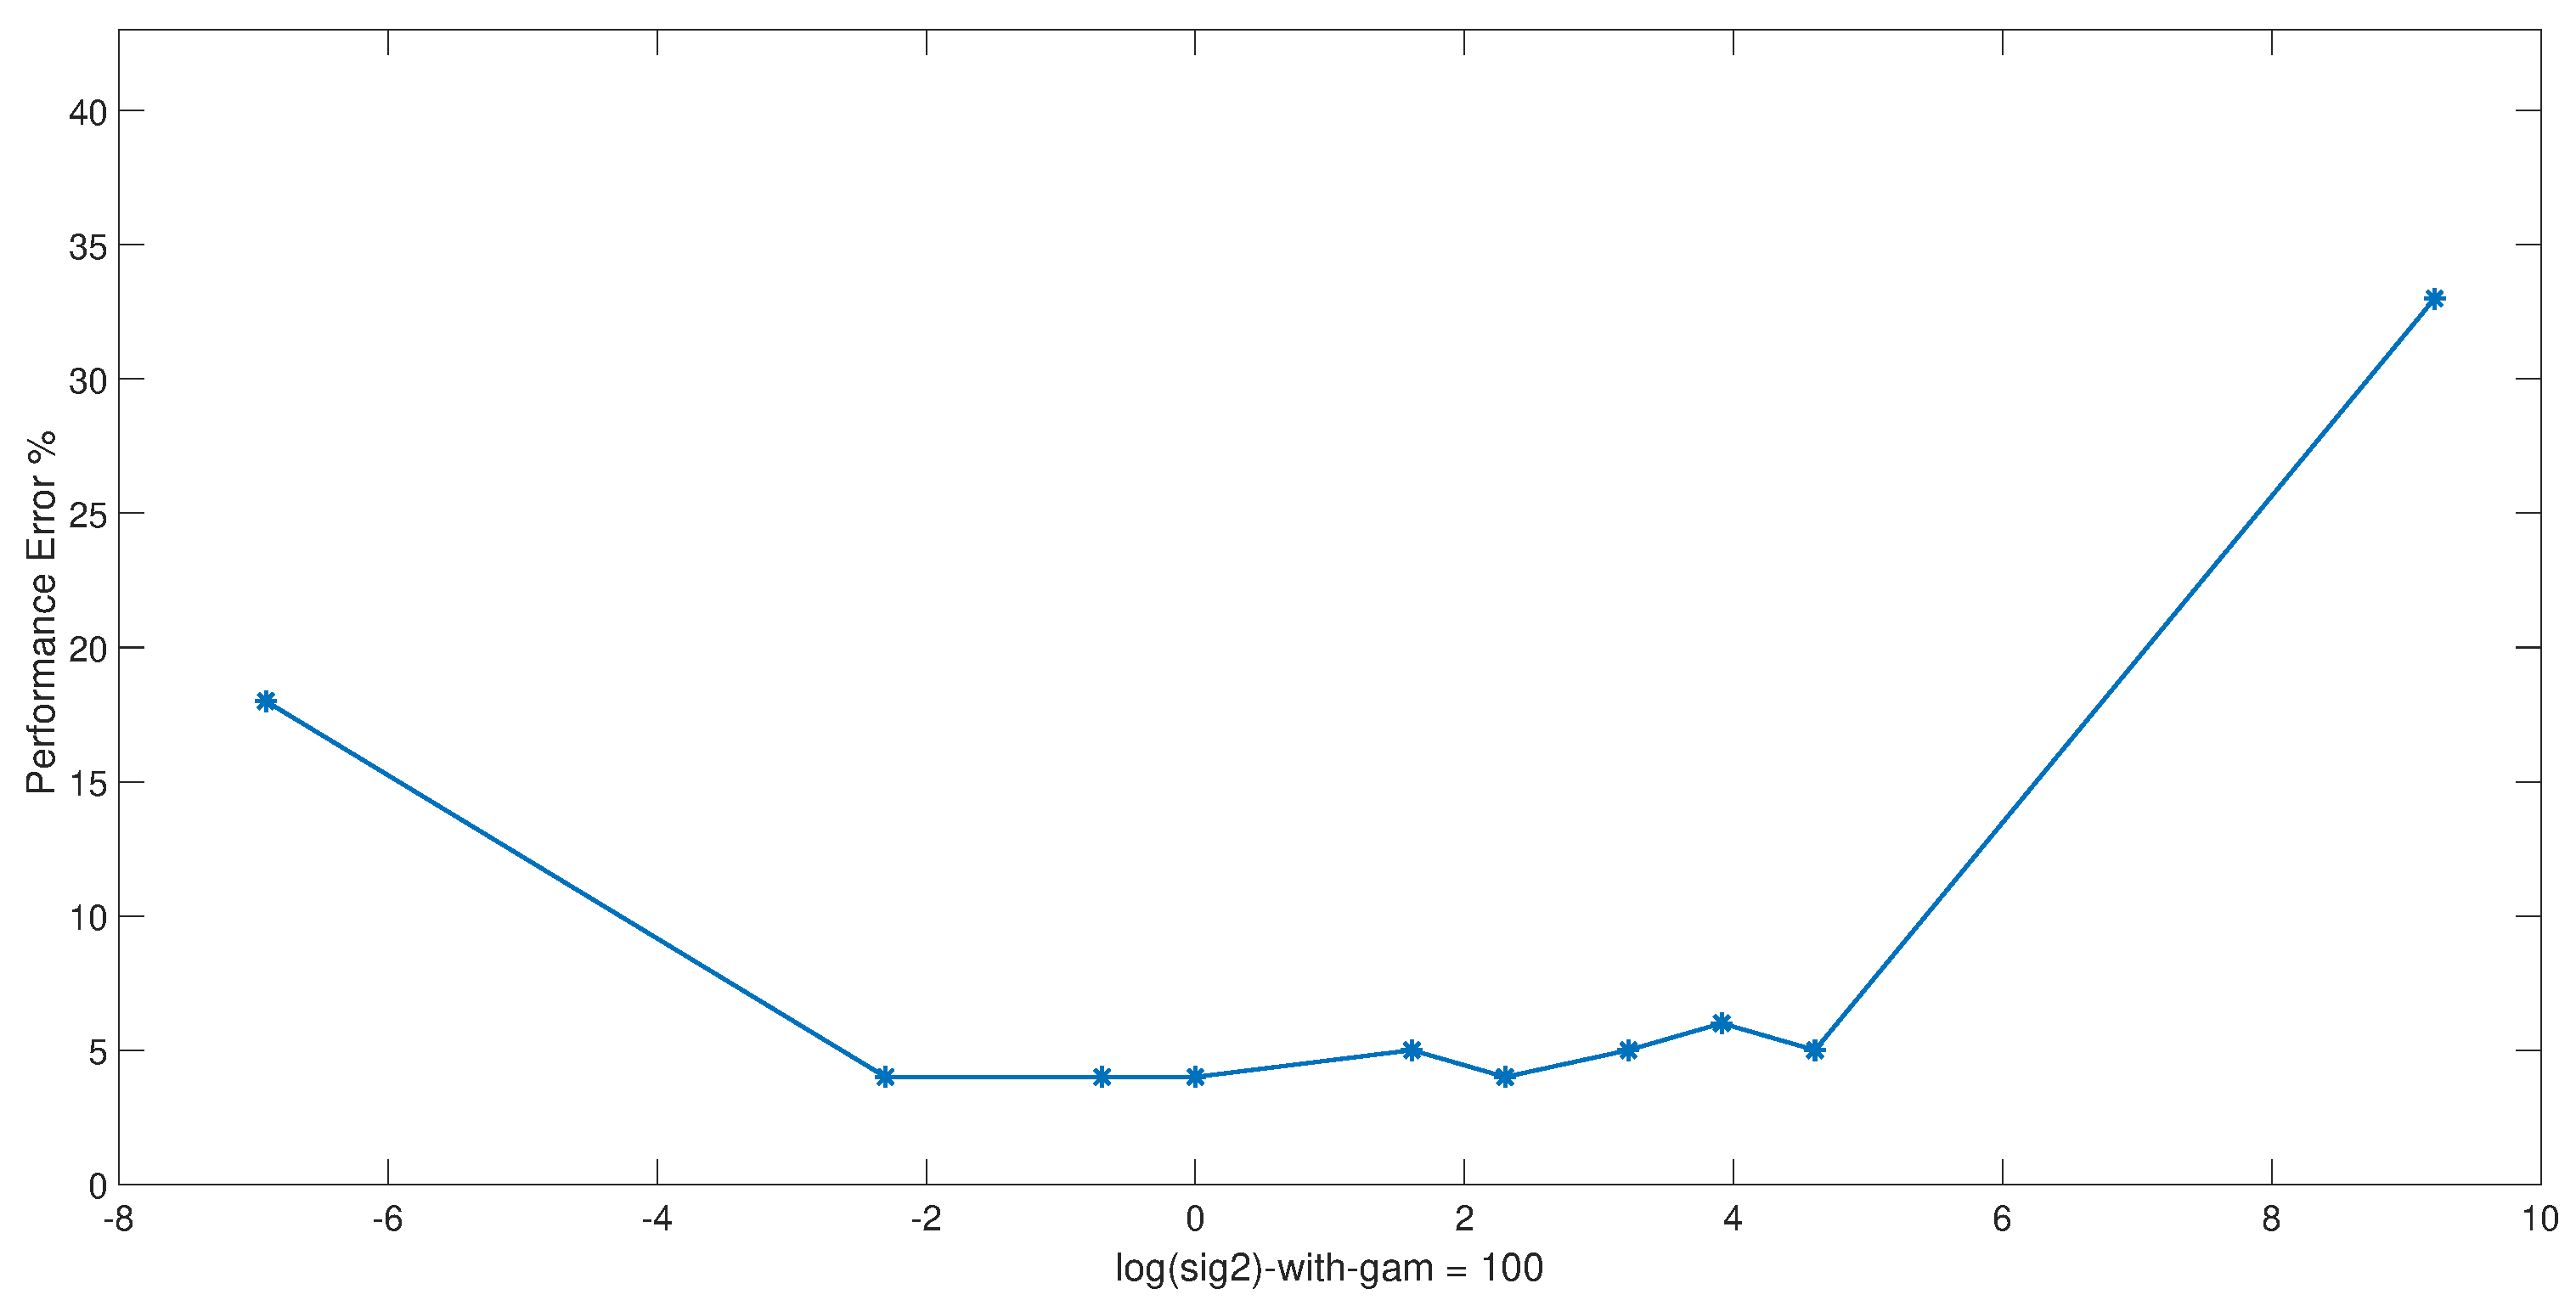
\includegraphics[height=0.35\linewidth,width=0.7\linewidth]{Exercise1/Report/Ex1.3_loo_gam(100).eps}
				\caption{$\gamma$ = 100}
				\label{fig:loo_gamma(100)}
			\end{subfigure}%
			\begin{subfigure}{.3\textwidth}
				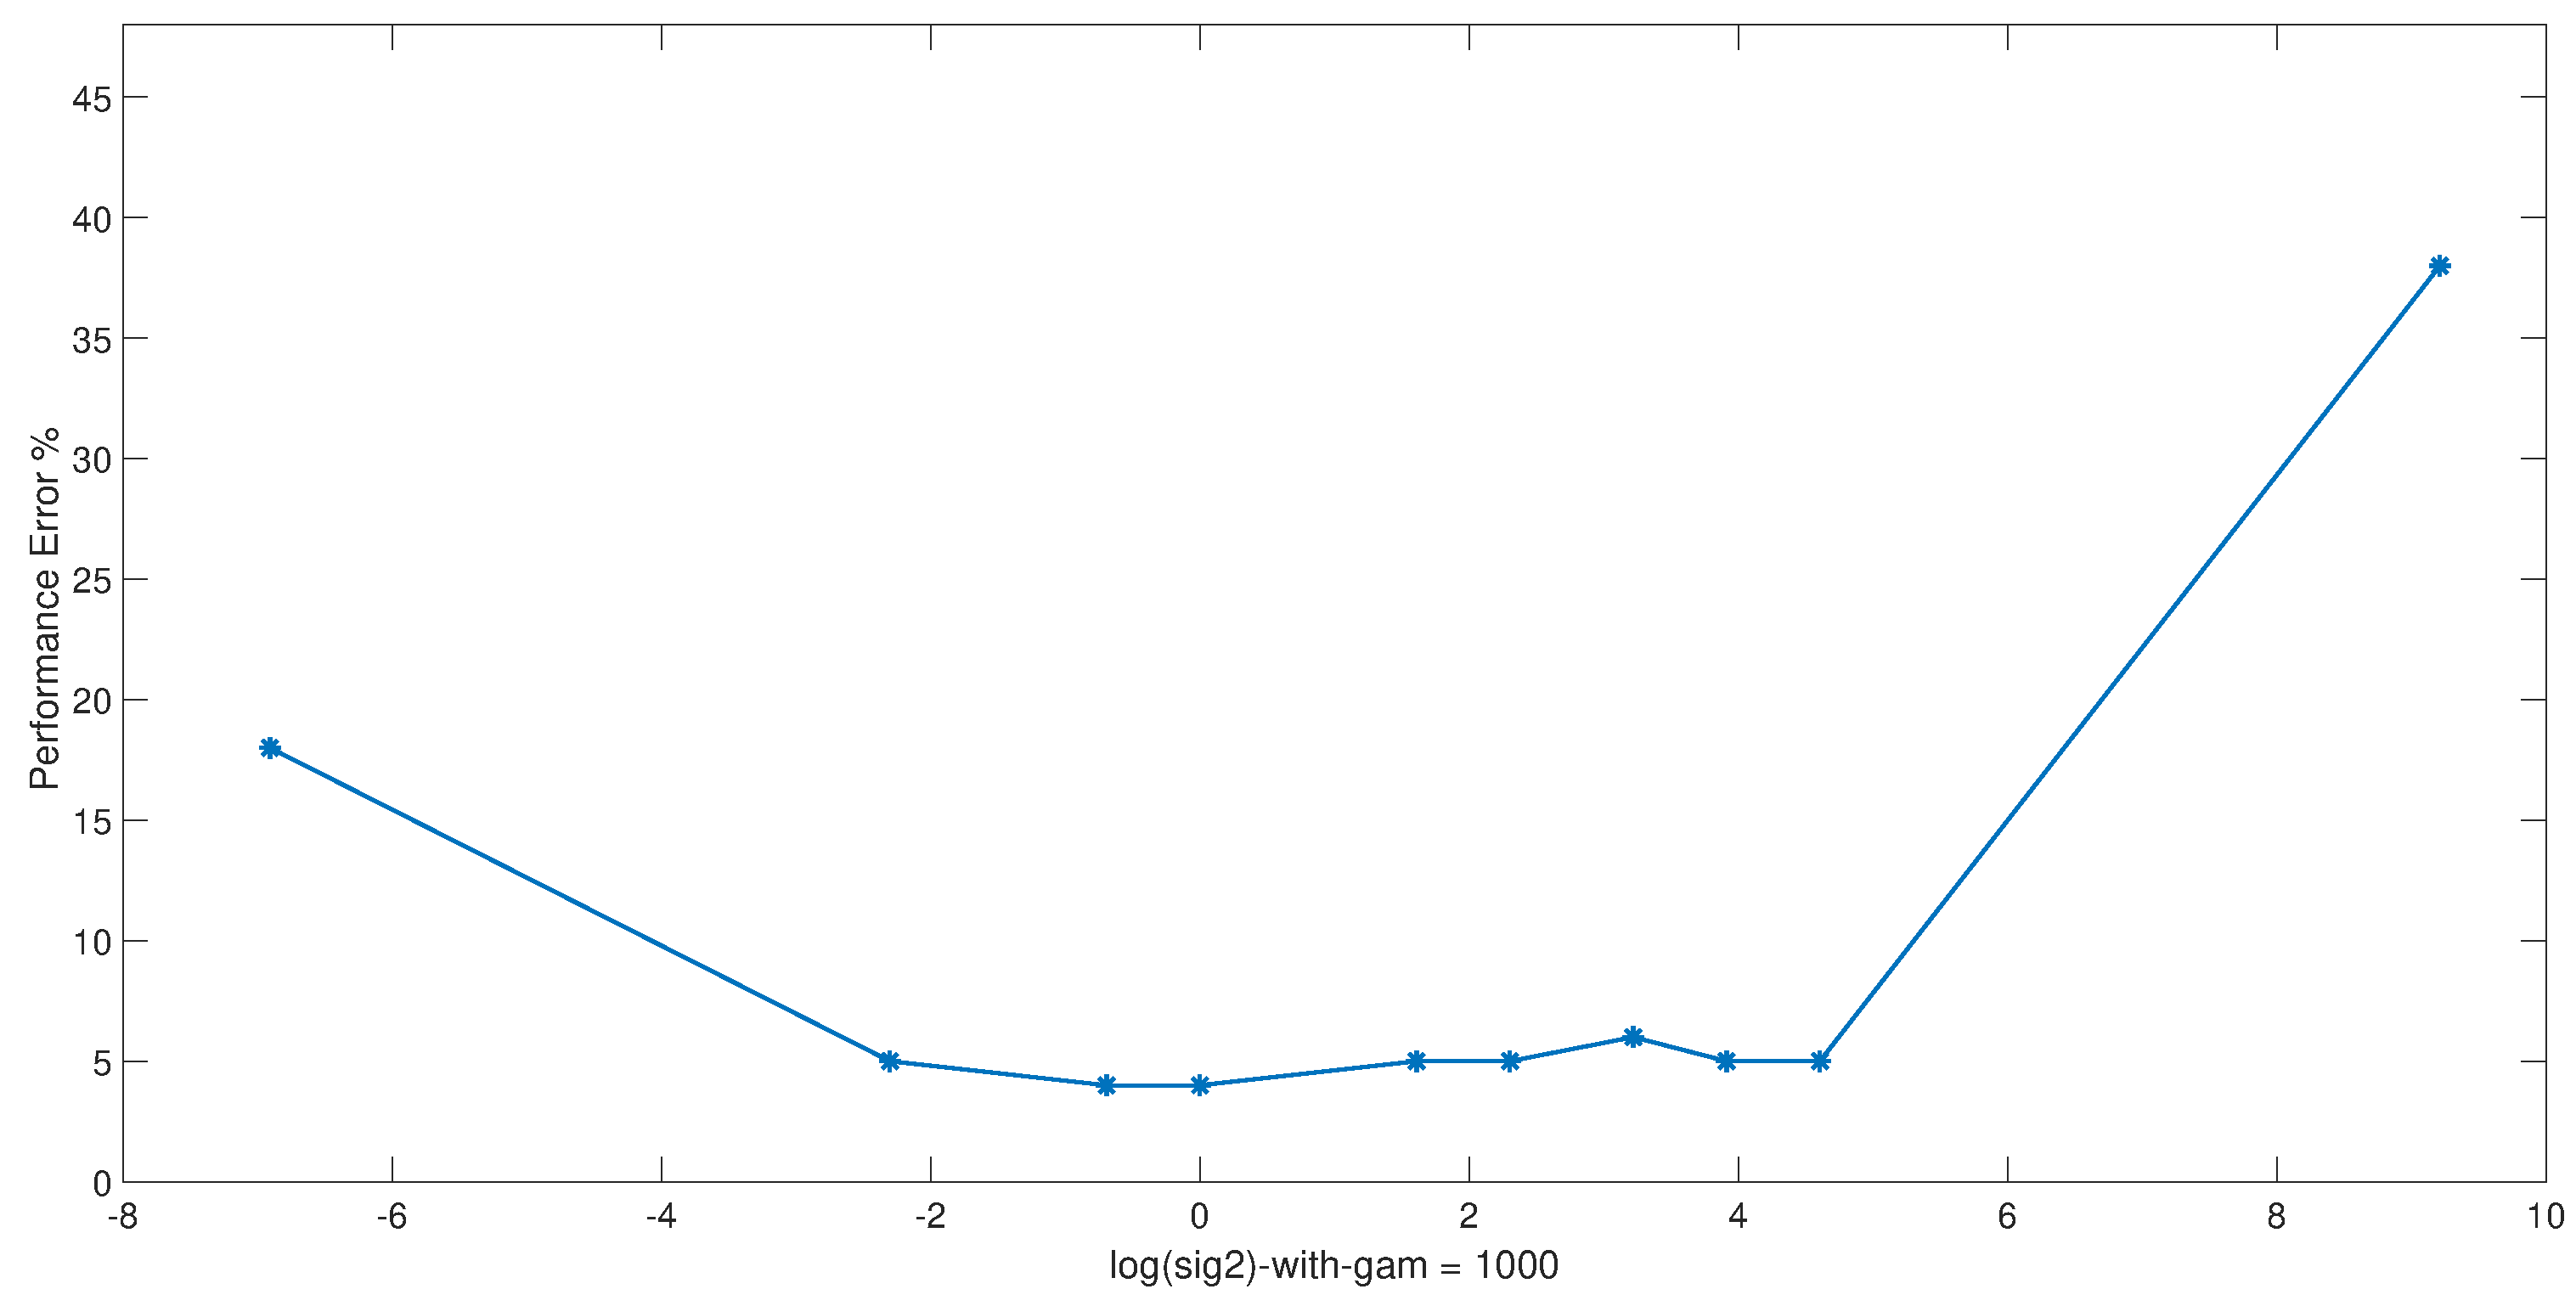
\includegraphics[height=0.35\linewidth,width=0.7\linewidth]{Exercise1/Report/Ex1.3_loo_gam(1000).eps}
				\caption{$\gamma$ = 1000}
				\label{fig:loo_gamma(1000)}
			\end{subfigure}%			
		}{%
			\caption{Iris data : LOOCV (log($\sigma^2$) values for each level of $\gamma$ Vs Performance Error)  (\%).}\label{fig:loo_gam}
		}
	\end{floatrow}
\end{figure}\\\\
\newline
\textbf{Why should one prefer crossvalidation over simple validation (random split)? How to choose the value of k in k-fold crossvalidation?}

In a cross validation method the model is  trained continuously k times over k-1 subsets of data
every time. By doing this the overall error of model is averaged over the errors for each iteration. The overall variance of the end result is small when compared with random split validation. This can be seen in figures \ref{fig:rand_3D} and \ref{fig:kCV_3D}. The value for k is chosen in a such way that the data samples in each set of k splits can statistically represent the original dataset. The choice of k influences the bias-variance trade-off. Factors like size of the data set, computational complexity, etc should also be taken into account while choosing k. For smaller data sets, a higher value of k is chosen so that the training sets have sufficient data samples. For larger data sets, a value of 10 can be chosen. In practice a value of 5 or 10 is chosen as optimal value as these values have proven to give unbiased results.
\subsubsection{Automatic parameter tuning}
\textbf{Try out the different ’algorithm’. What differences do you observe? Why do the obtained hyperparameters differ a lot in different runs? What about the cost? Computational speed? Explain the results.}

\begin{wraptable}[11]{l}{.7\textwidth}
	\begin{tabular}{ |p{1.5cm}|p{1.5cm}|p{1.5cm}||p{1.5cm}|p{1.5cm}|p{1.5cm}| }
		\hline
		\multicolumn{3}{|c|}{Simplex Algorithm} &\multicolumn{3}{|c|}{Grid Search Algorithm}
\\ \hline	
	\cellcolor{blue!25}$\gamma$ &\cellcolor{blue!25}$\sigma^2$ & \cellcolor{blue!25}cost & \cellcolor{blue!25}$\gamma$ &\cellcolor{blue!25}$\sigma^2$ &\cellcolor{blue!25}cost \\ \hline
	 3.54 &0.018991 &0.04 &18.165  &0.026866 &0.04 \\ \hline
	23.508 &0.34958 &0.04 &133.44  &0.024016 &0.02 \\ \hline
	0.4226 &0.18471 &0.04 &98.508  &63.077   &0.04 \\ \hline
	6.0573 &0.19643 &0.04 &3944.3  &0.32205  &0.03 \\ \hline
	106.55 &0.085258 &0.03 &0.2905 &0.020474 &0.03 \\ \hline
	12.893 &0.21712 &0.04 &11.129  &0.01182  &0.03 \\ \hline
	382.45 &0.28002 &0.03 &0.36295 &0.23467  &0.04 \\ \hline
	1.7285 &2.6992 &0.04 &0.046299 &0.41124  &0.04 \\ \hline
	\end{tabular}
	\caption{Optimal ($\gamma$, $\sigma^2$) pairs using auto tuning methods}
	\label{table:5}
\end{wraptable}

We train the SVM model again on Iris data set using tunelssvm for 8 iterations. The function trainlssvm performs 10-fold cross validation on training data and returns optimal values for $\gamma$ and $\sigma^2$. In previous section of tuning hyper-parameters, we saw that for a specific value of $\gamma$ a range of $\sigma$ works better (shown in table \ref{table:4}). How can we decide which pair of ($\gamma$, $\sigma^2$) is optimal. This is where the optimization algorithms simplex and grid search comes. They solve the convex-optimization problem for ($\gamma$,$\sigma^2$) and arrive at a local optima. We calculate the average time taken for each algorithm to give optimal values of ($\gamma$,$\sigma^2$). \\
Time taken to train SVM for 8 iterations using simplex algorithm is {\bf 3.058253 secs}.\\
Time taken to train SVM for 8 iterations using grid search algorithm is {\bf 6.016854 secs}.\\
We notice that simplex algorithm takes lesser time compared to grid search. This is because simplex tries to converge to the nearest local optima by initializing some random values to $\gamma$ and $\sigma^2$ whereas grid search evaluates over a range of parameters and then looks for the local optima.\\
From table \ref{table:5} it can be seen that the cost for all ($\gamma$,$\sigma^2$) pairs is around 0.02 to 0.04 which indicates that these pairs are optimal. As seen earlier in tuning hyper-parameters, the results show that many different ($\gamma$,$\sigma^2$) optimal pairs are possible. Therefore, the difference in ($\gamma$,$\sigma^2$) pairs for each run in auto tuning method is expected. 
\subsubsection{Using ROC Curves}
\textbf{ In practice, we compute the ROC curve on the test set, rather than on the training set. Why?}

ROC curves is one of the evaluation methods for the performance of a classifier. The classifier model is built using the training data. Evaluating the model for classification accuracy using training set will only give a biased estimate as the model has already seen the data samples. Therefore, the proper way to evaluate the classifier is using unseen data samples i.e., using test sets.\\\\
\textbf{Generate the ROC curve for the iris.mat dataset (use tuned gam and sig2 values). Interpret the result.}
\begin{figure}[!ht]
	\begin{subfigure}{0.5\linewidth}
		\centering
		\captionsetup{width=.8\linewidth}
		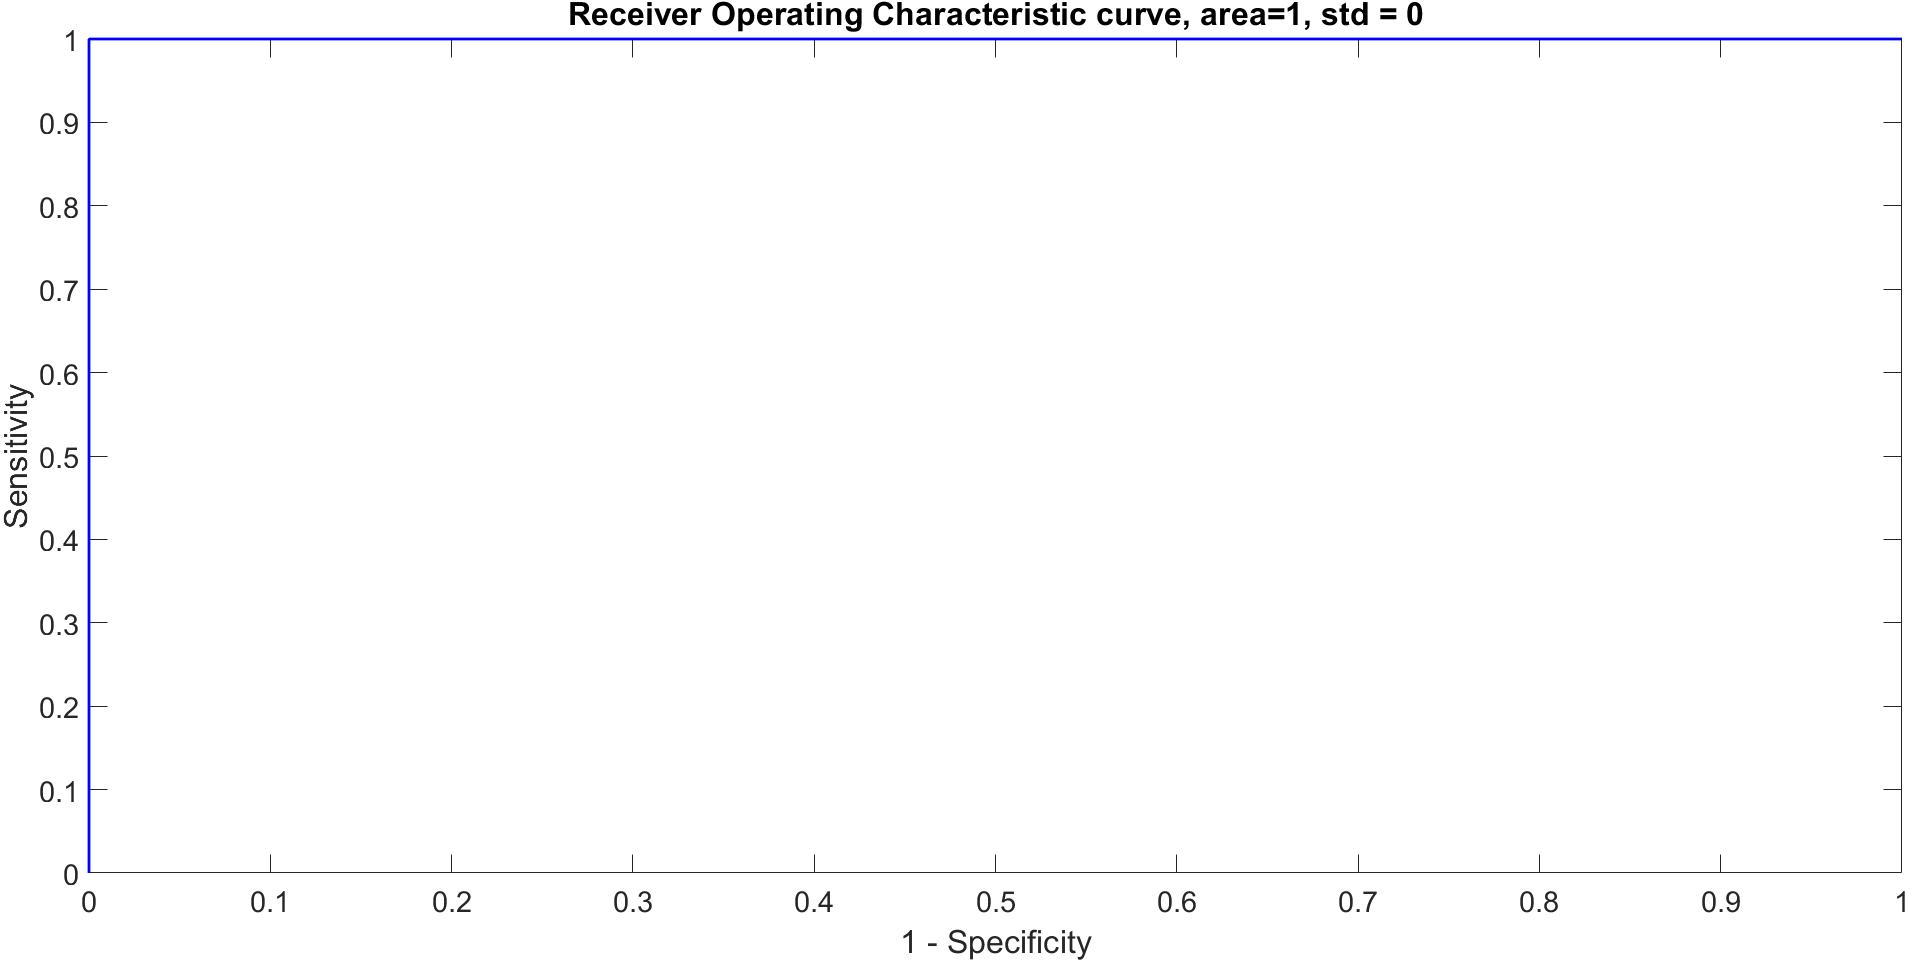
\includegraphics[width=0.8\linewidth]{Exercise1/Report/Ex1.3_ROC_simplex}
		\caption{ROC Curve with ($\gamma$,$\sigma^2$)=(6.0573,0.19643) obtained from auto tuning of hyper-parameters using simplex algorithm}
		\label{fig:ROC_simplex}\par\vfill
	\end{subfigure}%
	\begin{subfigure}{0.5\linewidth}
		\centering
		\captionsetup{width=.8\linewidth}
		\includegraphics[width=0.8\linewidth]{Exercise1/Report/EX1.3_ROC_grid.jpg}
		\caption{ROC Curve with ($\gamma$,$\sigma^2$)=(18.165,0.026866) obtained from auto tuning of hyper-parameters using grid search algorithm}
		\label{fig:ROC_grid}
	\end{subfigure}
	\caption{ROC Curves for SVM classifier with optimal ($\gamma$,$\sigma^2$) pairs}
	\label{fig:ROC}
\end{figure}

The ROC curves in the figure \ref{fig:ROC} tested on IRIS data set resembles an ideal classifier. Therefore, our SVM model built with optimal parameters of ($\gamma$,$\sigma^2$) pair is a perfect model.
\subsubsection{Bayesian framework}
\textbf{How do you interpret the colors of the plot? Change the values of gam and sig2. Visualize and discuss the influence of the parameters on the figure}

The Bayesian framework unlike other methods of SVM cannot give a strong decision boundary. Rather it gives the probability of an observation belonging to a target class based on prior and posterior probabilities of the data distribution. From the figures in fig \ref{fig:bayes}, it can be observed that the bayesian method gives two colors for each class (cyan - negative and magenta - positive) that slowly fade into one other indicating a separation of the two classes without a decision boundary. The colors here denote the probability of finding a positive class. As seen from the values of color bars next to each plot, it can be understood that magenta indicates the high probability of data points of positive class whereas cyan indicates the least probability of finding a positive class and vice versa. To get the results as show in figure \ref{fig:bayes}, the bayes framework is run first with a fixed value of $\gamma$ and varying value of $\sigma^2$ and then  with a fixed value of $\sigma^2$ and varying value of  $\gamma$.\\

 \begin{figure}[!htbp] 
	\centering
	\begin{subfigure}{.33\textwidth}
		\centering
		\includegraphics[height=0.8\linewidth,width=1\linewidth]{Exercise1/Report/Ex1.3.4_gam5_sig0.1.eps}
		\caption{($\gamma$ ; $\sigma^2$) = (5 ; 0.1)}
		\label{fig:gam5_sig0.1}
	\end{subfigure}%
	\begin{subfigure}{.33\textwidth}
		\centering
		\includegraphics[height=0.8\linewidth,width=1\linewidth]{Exercise1/Report/Ex1.3.4_gam5_sig1.eps}
		\caption{($\gamma$ ; $\sigma^2$) = (5 ; 1)}
		\label{fig:gam5_sig1}
	\end{subfigure}%
	\begin{subfigure}{.33\textwidth}
		\centering
		\includegraphics[height=0.8\linewidth,width=1\linewidth]{Exercise1/Report/Ex1.3.4_gam5_sig10.eps}
		\caption{($\gamma$ ; $\sigma^2$) = (5 ; 10)}
		\label{fig:gam5_sig10}
	\end{subfigure}
	\begin{subfigure}{.33\textwidth}
		\centering
		\includegraphics[height=0.8\linewidth,width=1\linewidth]{Exercise1/Report/Ex1.3.4_gam0.1_sig1.eps}
		\caption{($\gamma$ ; $\sigma^2$) = (0.1 ; 1)}
		\label{fig:gam0.1_sig1}
	\end{subfigure}%
	\begin{subfigure}{.33\textwidth}
		\centering
		\includegraphics[height=0.8\linewidth,width=1\linewidth]{Exercise1/Report/Ex1.3.4_gam3_sig1.eps}
		\caption{($\gamma$ ; $\sigma^2$) = (3 ; 1)}
		\label{fig:gam3_sig1}
	\end{subfigure}%
	\begin{subfigure}{.33\textwidth}
		\centering
		\includegraphics[height=0.8\linewidth,width=1\linewidth]{Exercise1/Report/Ex1.3.4_gam15_sig1.eps}
		\caption{($\gamma$ ; $\sigma^2$) = (15 ; 1)}
		\label{fig:gam15_sig1}
	\end{subfigure}%
	\caption{Bayesian Framework for various ($\gamma$ ; $\sigma^2$) values}
	\label{fig:bayes}
\end{figure}
The plots \ref{fig:gam5_sig0.1}, \ref{fig:gam5_sig1}. \ref{fig:gam5_sig10} is obtained by fixing the $\gamma$ value to 5 and varying the $\sigma^2$ values to (0.1; 1 ; 10). The plots \ref{fig:gam0.1_sig1}, \ref{fig:gam3_sig1}. \ref{fig:gam15_sig1} is obtained by fixing the $\sigma^2$ value to 1 and varying the $\gamma$ values to (0.1; 3 ; 15). It can be seen from the plots that for a higher value of $\gamma$ and lower value of $\sigma^2$, the model is able to accurately classify the data points of two classes. When $\sigma^2$ becomes greater than $\gamma$ ($\sigma^2$ $\geq$ 2$\gamma$) in fig \ref{fig:gam5_sig10} and \ref{fig:gam0.1_sig1} the cyan region becomes more dominant than magenta indicating a uncertainty in model. This leads to a lot of misclassifications. If the $\sigma^2$ values is made too small, the classification region can become too small trying to fit all the data points causing over fitting. Therefore, from these observations it can be said that it is preferred to have a balance between the values of ($\gamma$ ; $\sigma^2$) having a $\sigma^2$ value lesser than $\gamma$ for better performance of the model.   
\section{Homework Problems}
\subsection{Ripley Dataset}
\begin{wrapfigure}{l}{.4\textwidth}
	\begin{minipage}{\linewidth}
		\centering\captionsetup[subfigure]{justification=centering}
		\includegraphics[height = 0.5\linewidth, width=0.8\linewidth]{Exercise1/Report/ripley/ripley_train.eps}
		\subcaption{Training samples of ripley dataset}
		\label{fig:ripley_train}\par\vfill
		\includegraphics[height=0.5\linewidth,width=0.8\linewidth]{Exercise1/Report/ripley/ripley_test.eps}
		\subcaption{Test samples of ripley dataset}
		\label{fig:ripley_test}
	\end{minipage}
	\caption{Visualizing training and test samples of ripley data}
	\label{fig:ripley}
\end{wrapfigure}
The data set contains 250 training samples and 1000 test samples with only two features. Therefore, it is easy to visualize on a 2D plot. From the plot \ref{fig:ripley} it can be seen that the data not completely linearly separable as there are some overlaps between the two classes. So, a non-linear decision boundary can separate these two classes better than a linear one.  However, we train the SVM for linear , polynomial, RBF kernels and evaluate the models using ROC curves. The optimal hyper parameters of ($\gamma$, $\sigma^2$) for training is obtained using auto tuning method with simplex algorithm as seen in the earlier sections.\\
As seen from the figures \ref{fig:ripley_poly_svm}, \ref{fig:ripley_RBF_svm} the classifier with polynomial and RBF kernel performs in a similar way allowing only few misclassifications whereas the classifier with linear kernel gives few more misclassifications. In addition to this, the classifier is trained for few iterations with different optimal hyper parameters generated by \textit{tunelssvm} function and some of their results are evaluated and tabulated in \ref{table:6}. The results in table \ref{table:6} and  figures \ref{fig:ripley_lin_ROC}, \ref{fig:ripley_poly_ROC}, \ref{fig:ripley_RBF_ROC} show that, the classifier with RBF kernel gives slightly better accuracy (96.86 \% from ROC curve) than polynomial or linear kernels.
\begin{figure}[!ht] 
	\centering
	\begin{subfigure}{.35\textwidth}
		\centering
		\captionsetup{width=0.8\linewidth}
		\includegraphics[height=.65\linewidth, width=0.9\linewidth]{Exercise1/Report/ripley/ripley_lin_svm.eps}
		\caption{SVM with linear kernel- $\gamma$ = 0.0062614 }
		\label{fig:ripley_lin_svm}
	\end{subfigure}%
	\begin{subfigure}{.35\textwidth}
		\centering
		\captionsetup{width=0.8\linewidth}
		\includegraphics[height=.65\linewidth, width=0.9\linewidth]{Exercise1/Report/ripley/ripley_ploy_svm.eps}
		\caption{SVM with pol kernel- $\gamma$ = 3.0087 and degree = 5}
		\label{fig:ripley_poly_svm}
	\end{subfigure}%
	\begin{subfigure}{.35\textwidth}
		\centering
		\captionsetup{width=0.8\linewidth}
		\includegraphics[height=.65\linewidth, width=0.9\linewidth]{Exercise1/Report/ripley/ripley_RBF_svm.eps}
		\caption{SVM with RBF kernel- ($\gamma$, $\sigma^2$) =(3.3411, 0.72418) } 
		\label{fig:ripley_RBF_svm}
	\end{subfigure}
	\caption{SVM Classifier trained on Ripley dataset}
	\label{fig:ripley_svm}
\end{figure}
\begin{table}[!htpb]
	\begin{tabular}{ |p{1.2cm}|p{1.2cm}|p{1.2cm}||p{1.2cm}|p{1.2cm}|p{1.2cm}||p{1.2cm}|p{1.2cm}|p{1.2cm}|}
		\hline
		\multicolumn{3}{|c||}{Linear Kernel} &\multicolumn{3}{|c||}{Polynomial Kernel}  &\multicolumn{3}{|c|}{RBF Kernel} \\ \hline	
		\cellcolor{blue!25}$\gamma$ &\cellcolor{blue!25}$\sigma^2$ & \cellcolor{blue!25}Error & \cellcolor{blue!25}$\gamma$ &\cellcolor{blue!25}$\sigma^2$ &\cellcolor{blue!25}Error & \cellcolor{blue!25}$\gamma$ &\cellcolor{blue!25}$\sigma^2$ &\cellcolor{blue!25}Error \\ \hline
		0.00291 &-&10.6 &0.12909 &1.109 &10.2 &0.59161 &0.28572 &9.3 \\ \hline
		0.01678 &- &10.5 &3.0087 &2.0829 &10.1 &8.5381 &0.60447 &9.5 \\ \hline
	\end{tabular}
	\caption{SVM classifier on Ripley dataset - Performance results with different kernels for auto tuned hyper parameters}
	\label{table:6}
\end{table}
\begin{figure}[!ht] 
	\centering
	\begin{subfigure}{.35\textwidth}
		\centering
		\captionsetup{width=0.8\linewidth}
		\includegraphics[height=.65\linewidth, width=0.9\linewidth]{Exercise1/Report/ripley/ripley_lin_ROC.eps}
		\caption{ROC curve of SVM classifier with polynomial kernel}
		\label{fig:ripley_lin_ROC}
	\end{subfigure}%
	\begin{subfigure}{.35\textwidth}
		\centering
		\captionsetup{width=0.8\linewidth}
		\includegraphics[height=.65\linewidth, width=0.9\linewidth]{Exercise1/Report/ripley/ripley_poly_ROC.eps}
		\caption{ROC curve of SVM classifier with polynomial kernel}
		\label{fig:ripley_poly_ROC}
	\end{subfigure}%
	\begin{subfigure}{.35\textwidth}
		\centering
		\captionsetup{width=0.8\linewidth}
		\includegraphics[height=.65\linewidth, width=0.9\linewidth]{Exercise1/Report/ripley/ripley_RBF_ROC.eps}
		\caption{ROC curve of SVM classifier with RBF kernel} 
		\label{fig:ripley_RBF_ROC}
	\end{subfigure}
	\caption{ROC curves to evaluate SVM Classifier trained on Ripley dataset}
	\label{fig:ripley_ROC}
\end{figure}
\subsection{Wisconsin Breast Cancer dataset}
This data set contains   400 training samples and 169  test samples. There are 30 features in this dataset and is difficult to visualize on either 2D or 3D plots. As seen from the ROC curves in figure \ref{fig:breast_ROC}, the SVM classifier with linear and RBF kernels gives an accuracy greater than 99\%. This could be because of the reason that both the classes are well separated without many overlaps and the model is able to classify the test samples to the right class. Similar to the previous ripley data, the model is trained for few iterations with different optimal hyper parameters generated by \textit{tunelssvm} function and some of their results are evaluated and tabulated in \ref{table:7}. It is observed that the model performance remains more or less the same for change in hyper parameters in the case of linear and RBF kernels. For polynomial kernel, the model performs better for a degree of 3 than 5
\begin{figure}[!ht] 
	\centering
	\begin{subfigure}{.35\textwidth}
		\centering
		\captionsetup{width=0.8\linewidth}
		\includegraphics[height=.65\linewidth, width=0.9\linewidth]{Exercise1/Report/breast/breast_lin_ROC.eps}
		\caption{ROC curve of SVM classifier with polynomial kernel}
		\label{fig:breast_lin_ROC}
	\end{subfigure}%
	\begin{subfigure}{.35\textwidth}
		\centering
		\captionsetup{width=0.8\linewidth}
		\includegraphics[height=.65\linewidth, width=0.9\linewidth]{Exercise1/Report/breast/breast_poly_ROC.eps}
		\caption{ROC curve of SVM classifier with polynomial kernel}
		\label{fig:breast_poly_ROC}
	\end{subfigure}%
	\begin{subfigure}{.35\textwidth}
		\centering
		\captionsetup{width=0.8\linewidth}
		\includegraphics[height=.65\linewidth, width=0.9\linewidth]{Exercise1/Report/breast/breast_RBF_ROC.eps}
		\caption{ROC curve of SVM classifier with RBF kernel} 
		\label{fig:breast_RBF_ROC}
	\end{subfigure}
	\caption{ROC curves to evaluate SVM Classifier trained on breast cancer dataset}
	\label{fig:breast_ROC}
\end{figure}
\begin{table}[!htpb]
	\begin{tabular}{ |p{1.2cm}|p{1.2cm}|p{1.2cm}||p{2cm}|p{1.2cm}|p{1.2cm}||p{1.2cm}|p{1.2cm}|p{1.2cm}|}
		\hline
		\multicolumn{3}{|c||}{Linear Kernel} &\multicolumn{3}{|c||}{Polynomial Kernel}  &\multicolumn{3}{|c|}{RBF Kernel} \\ \hline	
		\cellcolor{blue!25}$\gamma$ &\cellcolor{blue!25}$\sigma^2$ & \cellcolor{blue!25}Error & \cellcolor{blue!25}$\gamma$ &\cellcolor{blue!25}degree &\cellcolor{blue!25}Error & \cellcolor{blue!25}$\gamma$ &\cellcolor{blue!25}$\sigma^2$ &\cellcolor{blue!25}Error \\ \hline
		0.07253 &-&4.7337 &1.533e-05 &3 &4.7337 &03.261 &37.617 &2.3669 \\ \hline
		8.2338 &- &4.7337 &2.0799e-07 &3  &3.5503 &22.922 &37.755 &1.7751 \\ \hline
		0.47591 &- &4.142 &182.19 &5 &15.976 &168.12 &44.754 &4.142 \\ \hline	
	\end{tabular}
	\caption{ SVM classifier on Breast Cancer dataset - Performance results with different kernels for auto tuned hyper parameters}
	\label{table:7}
\end{table}
\subsection{Diabetes dataset}
This data set contains   300 training samples and 168  test samples. There are 8 features in this dataset and is difficult to visualize on either 2D or 3D plots. As seen from the ROC curves in figure \ref{fig:breast_ROC}, the SVM classifier with polynomial kernel(fig \ref{fig:dia_poly_ROC}) performs with lesser accuracy(81.4 \%) compared with linear(fig \ref{fig:dia_lin_ROC}) and RBF kernels (\ref{fig:dia_RBF_ROC}) which gives an accuracy of 84\%. To investigate this performance accuracy of the model, two of the features were plotted and it is observed that the two classes have over lapping samples as shown in figure \ref{fig:dia_train}. Therefore, the model finds it difficult to generate a good decision boundary that separates these two classes with greater accuracy. Similar to the two previous data sets, the model is trained for few iterations with different optimal hyper parameters generated by \textit{tunelssvm} function and some of their results are evaluated and tabulated in \ref{table:8}. It is observed that the RBF kernel performs better and
the model performances of all three models remain more or less the same despite the change in hyper parameters. 
\begin{figure}[!ht] 
	\centering
	\begin{subfigure}{.35\textwidth}
		\centering
		\captionsetup{width=0.8\linewidth}
		\includegraphics[height=.65\linewidth, width=0.9\linewidth]{Exercise1/Report/diabetes/dia_lin_ROC.eps}
		\caption{ROC curve of SVM classifier with polynomial kernel}
		\label{fig:dia_lin_ROC}
	\end{subfigure}%
	\begin{subfigure}{.35\textwidth}
		\centering
		\captionsetup{width=0.8\linewidth}
		\includegraphics[height=.65\linewidth, width=0.9\linewidth]{Exercise1/Report/diabetes/dia_poly_ROC.eps}
		\caption{ROC curve of SVM classifier with polynomial kernel}
		\label{fig:dia_poly_ROC}
	\end{subfigure}%
	\begin{subfigure}{.35\textwidth}
		\centering
		\captionsetup{width=0.8\linewidth}
		\includegraphics[height=.65\linewidth, width=0.9\linewidth]{Exercise1/Report/diabetes/dia_RBF_ROC.eps}
		\caption{ROC curve of SVM classifier with RBF kernel} 
		\label{fig:dia_RBF_ROC}
	\end{subfigure}
	\caption{ROC curves to evaluate SVM Classifier trained on diabetes dataset}
	\label{fig:dia_ROC}
\end{figure}
 \begin{figure}[!ht]
	\begin{floatrow}
		\ffigbox[0.6\linewidth]
		{
			\includegraphics[height=0.7\linewidth,width= 0.8\linewidth]{Exercise1/Report/diabetes/dia_train.eps}
		}{
			\caption{Diabetes dataset}
			\label{fig:dia_train}
		}
		\capbtabbox{
			\begin{tabular}{ |p{1.cm}|p{1.cm}||p{1cm}|p{1cm}|p{1cm}||p{1cm}|p{1cm}|p{1cm}|}
				\hline
				\multicolumn{2}{|c||}{Linear Kernel} &\multicolumn{3}{|c||}{Polynomial Kernel}  &\multicolumn{3}{|c|}{RBF Kernel} \\ \hline	
				\cellcolor{blue!25}$\gamma$ & \cellcolor{blue!25}Error & \cellcolor{blue!25}$\gamma$ &\cellcolor{blue!25}degree &\cellcolor{blue!25}Error & \cellcolor{blue!25}$\gamma$ &\cellcolor{blue!25}$\sigma^2$ &\cellcolor{blue!25}Error \\ \hline
				0.0136 &25 &0.0020 &3 &29.167 &70.514 &253.93 &21.429 \\ \hline
				0.0176 &23.214 &1.2677 &3  &37.5 &191.73 &94556. &22.619 \\ \hline
				0.0090 &25 &0.0942 &3 &32.143 &4.149 &255.93 &22.619 \\ \hline	
			\end{tabular}
			
		}{
			\caption{SVM classifier on Diabetes dataset - Performance results with different kernels for auto tuned hyper parameters}
			\label{table:8}
		}
	\end{floatrow}
\end{figure}
	\chapter{Exercise 2: Function Estimation and Time Series Prediction}

\section{Support vector machine for function estimation}
\textbf{Construct a dataset where a linear kernel is better than any other kernel (around 20
	data points). What is the influence of e (try small values such as 0:10; 0:25; 0:50;..)
	and of Bound (try larger increments such as 0:01; 0:10; 1; 10; 100). Where does the
	sparsity property come in?}

The parameter $\epsilon$ controls the number of support vectors that the model takes to build the regression function. This in-turn determines width of the margin to fit the training data. Lower the value of $\epsilon$, higher the number of support vectors taken by that the model and vice versa. If $\epsilon$ values keeps increasing, the regressor fails to fit all the training data. This can be observed from the figures \ref{fig:lin_E=0.1_B=0.1}, \ref{fig:lin_E=0.3_B=0.1} and \ref{fig:lin_E=0.5_B=0.1} for a fixed bound value. On the other hand, we fix the value of $\epsilon$ and explore the regressor's performance for various values of bound. From figures \ref{fig:lin_E=0.15_B=0.01}, \ref{fig:lin_E=0.15_B=0.1} and \ref{fig:lin_E=0.15_B=10}m it can seen that the model performs poorly for lower value of bound and fits all the training data for higher value of bound.  Further increasing the bound value can cause the model to over-fit. It can be said that the bound is a trade-off between the error and model confidence. Sparsity comes into the picture when the model estimates better with less data points on unseen data. There won't be any sparseness in the model when it uses all the data points as support vectors. It is only possible for some optimal bound and $\epsilon$ say (0.15 and 0.1) as seen from figure \ref{fig:lin_E=0.15_B=0.1}.
\begin{figure}[ht]
	\centering
	\begin{subfigure}[b]{0.3\textwidth}
		\centering
		\includegraphics[width = 0.85\textwidth]{Exercise2/Report/Ex2.1_E=0.1_B=0.1}
		\caption{$\epsilon = 0.1$, Bound = 0.1 }\label{fig:lin_E=0.1_B=0.1}
	\end{subfigure}%
	\begin{subfigure}[b]{0.3\textwidth}
		\centering
		\includegraphics[width = 0.85\textwidth]{Exercise2/Report/Ex2.1_E=0.3_B=0.1}
		\caption{$\epsilon = 0.3$, Bound = 0.1 }\label{fig:lin_E=0.3_B=0.1}
	\end{subfigure}%
	\begin{subfigure}[b]{0.3\textwidth}
		\centering
		\includegraphics[width = 0.85\textwidth]{Exercise2/Report/Ex2.1_E=0.5_B=0.1}
		\caption{$\epsilon = 0.5$, Bound = 0.1 }\label{fig:lin_E=0.5_B=0.1}
	\end{subfigure}
	\begin{subfigure}[b]{0.3\textwidth}
		\centering
		\includegraphics[width = 0.85\textwidth]{Exercise2/Report/Ex2.1_E=0.15_B=0.01}
		\caption{$\epsilon = 0.15$, Bound = 0.01 }\label{fig:lin_E=0.15_B=0.01}
	\end{subfigure}%
	\begin{subfigure}[b]{0.3\textwidth}
		\centering
		\includegraphics[width = 0.85\textwidth]{Exercise2/Report/Ex2.1_E=0.15_B=0.1}
		\caption{$\epsilon = 0.15$, Bound = 0.1 }\label{fig:lin_E=0.15_B=0.1}
	\end{subfigure}%
	\begin{subfigure}[b]{0.3\textwidth}
		\centering
		\includegraphics[width = 0.85\textwidth]{Exercise2/Report/Ex2.1_E=0.15_B=10}
		\caption{$\epsilon = 0.15$, Bound = 10 }\label{fig:lin_E=0.15_B=10}
	\end{subfigure}
	\caption{SVM for Regression using Linear Kernel: demo \texttt{uiregress}. All the figures have same data points and performance of the regressor for different values of $\epsilon$ and bound are observed}
	\label{fig:uiregress_Linear}
\end{figure}\\
\textbf{Construct a more challenging dataset (around 20 data points). Which kernel is best
	suited for your dataset? Motivate why.}

Figure \ref{fig:uiregress_Kernels} shows the performance of the SVM regressor with different kernels on a challenging dataset for fixed values of $\epsilon$ and bound. Linear kernel as seen in figure \ref{fig:lin_E=0.6_B=inf} doesn't perform well. Polynomial kernels as seen from figures \ref{fig:Poly_deg=3_E=1_B=0.6} and \ref{fig:Poly_deg=5_E=1_B=0.6}, for degree = 3 doesn't perform well but for degree = 5 generalizes better. If the polynomial degree is increase the model over-fits. Figures \ref{fig:RBF_sig=0.05_E=1_B=0.6}, \ref{fig:RBF_sig=0.1_E=1_B=0.6} and \ref{fig:RBF_sig=1_E=1_B=0.6} shows the regressor with RBF kernel for various $\sigma^2$ values. For very lower values of $\sigma^2$, the model over-fits but for higher values the model gives a linear estimate. Therefore, for a value of $\sigma^2$ = 0.1, the model generalizes better. Overall the regressor with RBF kernel performs betters as it learns complex patterns of data better compared to a polynomial kernel.
\begin{figure}[ht]
	\centering
	\begin{subfigure}[b]{0.35\textwidth}
		\centering
		\captionsetup{width=0.8\linewidth}
		\includegraphics[width = 0.85\textwidth]{Exercise2/Report/Ex2.1_E=0.6_B=inf}
		\caption{Linear : $\epsilon = 0.6$, Bound = inf }\label{fig:lin_E=0.6_B=inf}
	\end{subfigure}%
	\begin{subfigure}[b]{0.35\textwidth}
		\centering
		\captionsetup{width=0.8\linewidth}
		\includegraphics[width = 0.85\textwidth]{Exercise2/Report/Ex2.1_Poly_deg=3_E=1_B=0.6}
		\caption{Poly : degree =3, $\epsilon = 1$, Bound = 0.6 }\label{fig:Poly_deg=3_E=1_B=0.6}
	\end{subfigure}%
	\begin{subfigure}[b]{0.35\textwidth}
		\centering
		\captionsetup{width=0.8\linewidth}
		\includegraphics[width = 0.85\textwidth]{Exercise2/Report/Ex2.1_Poly_deg=5_E=1_B=0.6}
		\caption{Poly : degree =5, $\epsilon = 1$, Bound = 0.6 }\label{fig:Poly_deg=5_E=1_B=0.6}
	\end{subfigure}
	\begin{subfigure}[b]{0.35\textwidth}
		\centering
		\captionsetup{width=0.8\linewidth}
		\includegraphics[width = 0.85\textwidth]{Exercise2/Report/Ex2.1_RBF_sig=0.05_E=1_B=0.6}
		\caption{RBF : $\sigma^2 = 0.05$ $\epsilon = 0.15$, Bound = 0.01 }\label{fig:RBF_sig=0.05_E=1_B=0.6}
	\end{subfigure}%
	\begin{subfigure}[b]{0.35\textwidth}
		\centering
		\captionsetup{width=0.8\linewidth}
		\includegraphics[width = 0.85\textwidth]{Exercise2/Report/Ex2.1_RBF_sig=0.1_E=1_B=0.6}
		\caption{RBF : $\sigma^2 = 0.1$ $\epsilon = 0.15$, Bound = 0.01 }\label{fig:RBF_sig=0.1_E=1_B=0.6}
	\end{subfigure}%
	\begin{subfigure}[b]{0.35\textwidth}
		\centering
		\captionsetup{width=0.8\linewidth}
		\includegraphics[width = 0.85\textwidth]{Exercise2/Report/Ex2.1_RBF_sig=1_E=1_B=0.6}
		\caption{RBF : $\sigma^2 = 1$ $\epsilon = 0.15$, Bound = 0.01 }\label{fig:RBF_sig=1_E=1_B=0.6}
	\end{subfigure}
	\caption{SVM for Regression using Linear, Polynomial and RBF Kernels: demo \texttt{uiregress}. }
	\label{fig:uiregress_Kernels}
\end{figure}\\
\textbf{In what respect is SVM regression different from a classical least squares fit?}

The difference in SVM regression and classical least squares is seen in loss function. Classical least squares use a L2 (squared) loss where as SVR uses a L1 loss with a threshold $\epsilon$. The observations outside this $\epsilon$ threshold is considered as points contributing to error.
\section{The sinc function}
\subsection{Regression of the sinc function}
\textbf{Try out a range of different gam and sig2 parameter values (e.g., gam = 10; $10^3$; $10^6$
	and sig2 = 0:01; 1; 100) and visualize the resulting function estimation on the test
	set data points. Discuss the resulting function estimation. Report the mean squared
	error for every combination ($\gamma$, $\sigma^2$).}

The SVM regressor model is trained using \textit{trainlssvm} function for various combinations of ($\gamma$ : $\sigma^2$) values and the results are plotted in figure \ref{fig:sinc_regress}. Also, MSE between the estimated and true results for every ($\gamma$ ; $\sigma^2$) pairs are tabulated in the table \ref{table:9}. From the figure and table it can be seen that the model performs well for ($\gamma$ ; $\sigma^2 $) values (1 ; 0.01), (1 ; 0.1), (10 ; 0.1). For larger values of $\sigma^2$, the model under performs on the dataset and gives poor estimates whereas for very low values it tries to overfit the data points. Therefore, a optimal pair of ($\gamma$, $\sigma^2$) should be such that $\gamma$ $>>$ $\sigma^2$ to get a small MSE between the ground truth and model estimates for the data points.\\
\begin{figure}[ht]
	\centering
	\begin{subfigure}[b]{0.35\textwidth}
		\centering
		\captionsetup{width=0.8\linewidth}
		\includegraphics[width = 0.85\textwidth]{Exercise2/Report/Ex_1_2_1_gam(10)_sig(0.01)}
		\caption{$\gamma = 10$ ; $\sigma^2 = 0.01$}\label{fig:Ex_1_2_1_gam(10)_sig(0.01)}
	\end{subfigure}%
	\begin{subfigure}[b]{0.35\textwidth}
		\centering
		\captionsetup{width=0.8\linewidth}
		\includegraphics[width = 0.85\textwidth]{Exercise2/Report/Ex_1_2_1_gam(10)_sig(0.1)}
		\caption{$\gamma = 10$ ; $\sigma^2 = 0.1$}\label{fig:Ex_1_2_1_gam(10)_sig(0.1)}
	\end{subfigure}%
	\begin{subfigure}[b]{0.35\textwidth}
		\centering
		\captionsetup{width=0.8\linewidth}
		\includegraphics[width = 0.85\textwidth]{Exercise2/Report/Ex_1_2_1_gam(10)_sig(10)}
		\caption{$\gamma = 10$ ; $\sigma^2 = 10$}\label{fig:Ex_1_2_1_gam(10)_sig(10)}
	\end{subfigure}
	\begin{subfigure}[b]{0.35\textwidth}
		\centering
		\captionsetup{width=0.8\linewidth}
		\includegraphics[width = 0.85\textwidth]{Exercise2/Report/Ex_1_2_1_gam(0.1)_sig(0.1)}
		\caption{$\gamma = 0.1$ ; $\sigma^2 = 0.1$}\label{fig:Ex_1_2_1_gam(0.1)_sig(0.1)}
	\end{subfigure}%
	\begin{subfigure}[b]{0.35\textwidth}
		\centering
		\captionsetup{width=0.8\linewidth}
		\includegraphics[width = 0.85\textwidth]{Exercise2/Report/Ex_1_2_1_gam(10)_sig(0.1)}
		\caption{$\gamma = 10$ ; $\sigma^2 = 0.1$ }\label{fig:Ex_1_2_1_gam(1)_sig(0.1)}
	\end{subfigure}%
	\begin{subfigure}[b]{0.35\textwidth}
		\centering
		\captionsetup{width=0.8\linewidth}
		\includegraphics[width = 0.85\textwidth]{Exercise2/Report/Ex_1_2_1_gam(10000)_sig(0.1)}
		\caption{$\gamma = 10000$ ; $\sigma^2 = 0.1$}\label{fig:Ex_1_2_1_gam(10000)_sig(0.1)}
	\end{subfigure}
	\caption{SVM Regressor : Function estimation for various ($\gamma$; $\sigma^2$) values of the RBF kernel}
	\label{fig:sinc_regress}
\end{figure}
\begin{table}[!htpb]
	\centering
	\begin{tabular}{ ||p{1.8cm}||p{1.8cm}|p{1.8cm}|p{1.8cm}|p{1.8cm}|p{1.8cm}|p{1.8cm}|}
		\hline
		\multicolumn{7}{|c|}{Mean Squared Error (MSE) (\%)} \\ \hline\hline
		\cellcolor{blue!25}($\gamma$ ; $\sigma^2$) &\cellcolor{blue!25}$\sigma^2 = 0.01$ & \cellcolor{blue!25}$\sigma^2 = 0.1$ &\cellcolor{blue!25}$\sigma^2 = 1$ & \cellcolor{blue!25}$\sigma^2 = 10$ &\cellcolor{blue!25}$\sigma^2 = 10^2$ &\cellcolor{blue!25}$\sigma^2 = 10^3$ \\ \hline \hline
		\cellcolor{blue!25}$\gamma = 0.1$ &2.2498&1.5692&8.3871&12.988&13.631&13.641 \\ \hline
		\cellcolor{blue!25}$\gamma = 1$ &1.1784&1.1024&5.1397&11.392&13.553&13.639 \\ \hline
		\cellcolor{blue!25}$\gamma = 10$ &1.2326&1.121&3.261&10.967&12.937&13.631 \\ \hline
		\cellcolor{blue!25}$\gamma = 10^2$ &1.2621&1.1367&1.481&10.526&11.474&13.552 \\ \hline
		\cellcolor{blue!25}$\gamma = 10^3$ &1.2758&1.1503&1.2254&8.2999&11.205&12.932 \\ \hline
		\cellcolor{blue!25}$\gamma = 10^4$ &1.2791&1.1612&1.1065&6.659&11.201&11.483 \\ \hline
	\end{tabular}
	\caption{MSE (\%) between SVR estimations and ground truth data for various ($\gamma$ ; $\sigma^2$)}
	\label{table:9}
\end{table}\\
\textbf{Do you think there is one optimal pair of hyperparameters? }

As seen from figure \ref{fig:sinc_regress} and table \ref{table:9}, it can be inferred that the model performs better and have least MSE for lower values of $\sigma^2$ such as 0.01 and 0.1 for $\gamma$ in range of 1 to $10^4)$.  One such optimal pair can be  ($\gamma$, $\sigma^2$) = (1 ; 0.1) and (10;0.1)\\
\newline
\textbf{Tune the gam and sig2 parameters using the tunelssvm procedure. Use multiple runs:
	what can you say about the hyperparameters and the results? Use both the simplex
	and gridsearch algorithms and report differences.}

\begin{wraptable}[11]{l}{.7\textwidth}
	\centering
	\begin{tabular}{ |p{1.5cm}|p{1.5cm}|p{1.7cm}||p{1.5cm}|p{1.5cm}|p{1.7cm}| }
		\hline
		\multicolumn{3}{|c||}{Simplex Algorithm} &\multicolumn{3}{c|}{Grid Search Algorithm}
		\\ \hline	
		\cellcolor{blue!25}$\gamma$ &\cellcolor{blue!25}$\sigma^2$ & \cellcolor{blue!25}cost & \cellcolor{blue!25}$\gamma$ &\cellcolor{blue!25}$\sigma^2$ &\cellcolor{blue!25}cost \\ \hline
		44.681 &0.36072 &0.0099951 &222.33 &0.44703 &0.0098997 \\ \hline
		390.57 &0.48974 &0.010855 &21.733  &0.33129 &0.010041 \\ \hline
		46.424 &0.38045 &0.010003 &44.117  &0.3663   &0.0099097 \\ \hline
		76.299 & 0.39569 &0.010843 &23.237  &0.34383  &0.0099472 \\ \hline
		57.125 &0.39352 &0.0099651 &16.346 &0.31191 &0.010876 \\ \hline
		
	\end{tabular}
	\caption{Optimal ($\gamma$, $\sigma^2$) pairs using auto tuning methods}
	\label{table:10}
\end{wraptable}
From table \ref{table:10} it can seen that both the algorithms produce different optimal ($\gamma$;$\sigma^2$) for each run but the error approximately remains the same. Also, a lot of variability is seen only in $\gamma$ values whereas $\sigma^2$ has much lesser variance. Overall, it can be said that $\gamma$ $>>$ $\sigma^2$. Also, simplex algorithm executes faster with 0.85 secs compared to grid search method which takes 1.2 sec approximately. 
\subsection{Application of the Bayesian framework}
\textbf{Discuss in a schematic way how parameter tuning works using the Bayesian framework.
	Illustrate this scheme by interpreting the function calls denoted above.}

\begin{figure}[ht]
	\centering
	\begin{subfigure}[b]{0.5\textwidth}
		\centering
		\captionsetup{width=0.7\linewidth}
		\includegraphics[height = 0.5\linewidth, width=0.8\linewidth]{Exercise2/Report/Bayesian_1.eps}
		\caption{Bayes Framework: LS-SVM with ($\gamma$,$\sigma^2$)=(10,0.4)}
		\label{fig:Bayesian_1}
	\end{subfigure}%
	\begin{subfigure}[b]{0.5\textwidth}
		\centering
		\captionsetup{width=0.7\linewidth}
		\includegraphics[height = 0.5\linewidth, width=0.8\linewidth]{Exercise2/Report/Bayesian_2.eps}
		\caption{Bayes Framework: LS-SVM with ($\gamma$,$\sigma^2$) obtained from auto tune method}
	\label{fig:Bayesian_2}
	\end{subfigure}

	\caption{Bayesian Framework : LS-SVM }	\label{fig:bayes_1}
\end{figure}
In this section we analyze the function estimation in Bayesian Framework. We first initialize ($\gamma$,$\sigma^2$) values as (10,0.4). We obtain the corresponding posterior parameters as (0.41251, 0.26488) and MSE as 0.1957.  Instead of these random ($\gamma$;$\sigma^2$), we obtain the optimal hyperparameter values using \textit{tunelssvm} with simplex algorithm as (25.6337 ; 0.3815). With these settings we get the posterior parameters as (7.8817; 0.31367) and MSE 0.0423 after bayesian optimization. The corresponding plots are given in figure \ref{fig:bayes_1}.

The optimization in bayesian learning happens in three levels. We assign a probability over all the values of the weight vector $w$ instead of single point of the vector space. For this we need to a prior $p(w)$ and a likelihood                                                                                                                                                                                                                                                                                                                                                                                                                                                                                                                                                                                                                                                                                                                                                                                                                                                                                                                                                                                                                                                                                                                                                                                                                                                                                                                                                                                                                                                                                                                                                                                                                                                                                                                                                                                                                                                                                                                                                                                                                                                                                                                                                                                                                                                                                                                                                                                                                                                                                                                                                                                                                                                                                                                                                                                                                                        probabilities $p(D|w)$ over the data distribution $D$. The posterior probability distribution  can be obtained from prior and likelihood as $P(w|D)=\frac{P(D|w)P(w)}{P(D}$.

\textbf{Level 1:} The main objective here is to minimize the weight space parameters $w$ and $b$. The LS-SVM also includes the regularization hyperparameters $\mu$ and $\zeta$ in its objective function as shown in the below equation \ref{eq:2.1}. Here the optimization is done for $w$ and the bias $b$.

\begin{equation}\label{eq:2.1}
\min\limits_{w,b,e_c} J_P(w,e_c) = \mu \frac{1}{2}w^Tw + \zeta \sum_{k=1}^{N}e_{c,k}^2
\end{equation} 
In the above equation the first term corresponds to prior distribution and the second term corresponds to the likelihood. The posterior distribution and the model $H_\sigma$ is given by:

\begin{equation}\label{eq:2.2}
p(w,b|D,\mu,\zeta,H_\sigma) = \frac{p(D|w,b,\mu,\zeta,H_\sigma)}{p(D|\mu,\zeta,H_\sigma)}p(w,b|\mu,\zeta,H_\sigma)
\end{equation}
Minimization of equation \ref{eq:2.1} for $\mu$, $w$ and $\zeta$ gives the maximization of equation \ref{eq:2.2}. 

\textbf{Level 2:} The regularization parameters $\mu$ and $\zeta$ are optimized in second level.

\textbf{Level 3:} In level three the optimization is done for the kernel parameters. It can used for model selection. 

Therefore, as shown in figure \ref{fig:Bayesian_2}, it results in a better performance for the bayesian framework when tuned with optimal hyperparameters and optimization as MSE given by that model is very less.
\section{Automatic Relevance Determination}
 \begin{figure}[!ht]
	\begin{floatrow}
		\ffigbox{%
			\centering
				\includegraphics[height = 0.5\textwidth, width = 0.6\textwidth]{Exercise2/Report/Bayes_ARD_1} %
		}{%
			
			\caption{Data distribution}\label{fig:Bayes_ARD_1}%
		}
		\ffigbox{%
			\begin{subfigure}[b]{0.35\textwidth}
				\centering
				\captionsetup{width=1\linewidth}
				\includegraphics[width = 1\textwidth]{Exercise2/Report/Bayes_ARD_2}
				\caption{Bayes ARD ranking for ($\gamma$;$\sigma^2$)=(10,0.4)}\label{fig:Bayes_ARD_2}
			\end{subfigure}
			\begin{subfigure}[b]{0.35\textwidth}
				\centering
				\captionsetup{width=1\linewidth}
				\includegraphics[width = 1\textwidth]{Exercise2/Report/Bayes_ARD_3}
				\caption{Bayes ARD ranking for ($\gamma$;$\sigma^2$) selected from cross validation}\label{fig:Bayes_ARD_3}
			\end{subfigure}			
		}{%
		\caption{Bayes : ARD}
		\label{fig:Bayes_ARD}
		}
	\end{floatrow}
\end{figure}
The Automatic Relevance Distribution ranks the best input data distribution that fits the target by estimating the hyper parameters. To illustrate this, we build three random data distributions X1, X2 and X3.The target label Y is built from X1. The result of figure \ref{fig:Bayes_ARD_2}, is plotted for the model built by randomly choosing ($\gamma$;$\sigma^2$) pair. In figure \ref{fig:Bayes_ARD_3}, the model is built by selecting the inputs using cross validation. As seen from figures \ref{fig:Bayes_ARD_1} and \ref{fig:Bayes_ARD}, the ARD algorithm in both cases gives the data X1 and the most relevant one which is obvious as Y corresponds to X1. Similar results are seen when changing the target Y corresponding to X2 and X3 distributions.   
\section{Robust regression}
\textbf{Visualize and discuss the results. Compare the non-robust version with the robust
	version. Do you spot any differences?}

The figure \ref{fig:robust} shows robust vs non-robust LS-SVM estimations for data points with and without outliers. The non-robust regressor with outliers fail to perform well as the estimations try to take the outliers also into account. This results in a poor fit over the data points as seen in figure \ref{fig:rob_outliers}. On the other hand, the robust regressor with cross validation gives good performance with better function estimations ignoring the outliers as seen in figure \ref{fig:rob_huber}\\\\
\begin{figure}[!ht] 
	\begin{subfigure}{.35\textwidth}
		\centering
		\captionsetup{width=0.8\linewidth}
		\includegraphics[height=.65\linewidth, width=0.9\linewidth]{Exercise2/Report/robust_withoutOutliers}
		\caption{LS-SVM Regressor : Without Outliers}
		\label{fig:rob_nooutliers}
	\end{subfigure}%
	\begin{subfigure}{.35\textwidth}
		\centering
		\captionsetup{width=0.8\linewidth}
		\includegraphics[height=.65\linewidth, width=0.9\linewidth]{Exercise2/Report/robust_withOutliers}
		\caption{LS-SVM Regressor : With Outliers}
		\label{fig:rob_outliers}
	\end{subfigure}%
	\begin{subfigure}{.35\textwidth}
		\centering
		\captionsetup{width=0.8\linewidth}
		\includegraphics[height=.65\linewidth, width=0.9\linewidth]{Exercise2/Report/robust_huber}
		\caption{LS-SVM Regressor : Robust Cross Validation}
		\label{fig:rob_huber}
	\end{subfigure}
	\caption{LS-SVM : Robust Vs Non-Robust versions}
	\label{fig:robust}
\end{figure}
\textbf{Why in this case is the mean absolute error (’mae’) preferred over the classical mean
	squared error (’mse’)?}

MAE is the measure of average magnitude of errors between true and estimated data points. Whereas MSE is the measure of squared average magnitude of errors. Since, MSE is the squared error, it adds more weight to outliers where the errors are high.This makes the model perform poorly when trying to minimize the errors. This is not the case with MAE as it only takes the absolute average of errors and that makes it more robust to outliers.
\begin{align*}
MAE = \frac{1}{N} \sum_{i=1}^{N} |y_i - \hat{y_i}| && MSE = \frac{1}{N} \sum_{i=1}^{N} (y_i - \hat{y_i})^2 \label{eq:label1}
\end{align*}\\
\textbf{Try alternatives to the weighting function wFun (e.g., ’whampel’, ’wlogistic’ and
	’wmyriad’. Report on differences. Check the user’s guide of LS-SVMlab for more
	information.}
\begin{figure}[!ht] 
	\begin{subfigure}{.35\textwidth}
		\centering
		\captionsetup{width=0.8\linewidth}
		\includegraphics[height=.65\linewidth, width=0.9\linewidth]{Exercise2/Report/robust_logistic}
		\caption{Robust LS-SVM Regressor : Logistic}
		\label{fig:rob_nooutliers}
	\end{subfigure}%
	\begin{subfigure}{.35\textwidth}
		\centering
		\captionsetup{width=0.8\linewidth}
		\includegraphics[height=.65\linewidth, width=0.9\linewidth]{Exercise2/Report/robust_myriad}
		\caption{Robust LS-SVM Regressor : Myriad}
		\label{fig:rob_myriad}
	\end{subfigure}%
	\begin{subfigure}{.35\textwidth}
		\centering
		\captionsetup{width=0.8\linewidth}
		\includegraphics[height=.65\linewidth, width=0.9\linewidth]{Exercise2/Report/robust_hampel}
		\caption{Robust LS-SVM Regressor : Hampel}
		\label{fig:rob_hampel}
	\end{subfigure}
	\caption{LS-SVM : Robust versions with different weighting functions}
	\label{fig:robust_versions}
\end{figure}
\begin{table}[!htpb]
	\centering
	\begin{tabular}{ |p{4.5cm}||p{2.5cm}||p{2.5cm}||p{2.5cm}||p{2.5cm}|}
		\hline
		\cellcolor{blue!25} Weighting Function &\cellcolor{blue!25}$\gamma$ &\cellcolor{blue!25}$\sigma^2$ & \cellcolor{blue!25} Iterations for convergence & \cellcolor{blue!25} Cost \\ \hline
		\cellcolor{blue!25} wHuber  &12190.9097 & 0.10022 & 112 & 1.368683e-01 \\ \hline
		\cellcolor{blue!25} wLogistic &101.6236 & 0.081962 & 62&1.392045e-01  \\ \hline
		\cellcolor{blue!25} wMyriad & 11.4796&0.025126 & 13& 1.339679e-01 \\ \hline
		\cellcolor{blue!25} wHampel & 17.26 & 0.034283 & 4 & 1.360631e-01 \\ \hline
	\end{tabular}
	\caption{LS-SVM Robust Regressor with different weighting functions and their optimal hyper parameters ($\gamma$;$\sigma^2$)}
	\label{table:11}
\end{table}

The estimations of robust LS-SVM for various weighting functions are plotted in figure \ref{fig:robust_versions} and the results are given in the table \ref{table:11}. From the table \ref{table:11}, it can be seen that Hampel is faster as it achieves the convergence with only 4 iterations and Huber is the slowest. But, as seen from cost, the overall performance of all the weighting functions remain same. Every model gives approximately same estimations over the training data ignoring the outliers.
\section{Homework Problems}
\subsection{Logmap dataset}

\begin{wrapfigure}{L}{0.5\textwidth}
	\begin{center}
		\includegraphics[height=0.5\linewidth,width= 1\linewidth]{Exercise2/Report/HWOriginal.eps} 
		\caption{LS-SVM: Logmap Dataset with ($\gamma$;$\sigma^2$)=(10;10)}
		\label{fig:hw1}
	\end{center}
\end{wrapfigure}
In this section, we follow the instructions given in the exercise to obtain a model fit on the logmap dataset. From figure \ref{fig:hw1} it can be noticed that for initial ($\gamma$;$\sigma^2$) values of (10;10), the model estimates are very poor. The predictions fit the ground truth data only between the range 22 to 30. To get better model performance we use auto tune methods and cross validation method to obtain the optimal hyper parameters ($\gamma$;$\sigma^2$). For the lag parameter, we try out a range from 1 to 50 with each of the obtained optimal ($\gamma$;$\sigma^2$) pairs. The best fit obtained from the model is plotted in the figure \ref{fig:hw2}. The optimal values of ($\gamma$;$\sigma^2$) and the lag is chosen by calculating MAE of the model on the test set for which the MAE $\leq$ 15. The model estimates are not completely perfect as it fails to fit at the huge peaks of the data set. The plots shown in figure \ref{fig:hw2} are the ones with the least MAE values.
\begin{figure}[!ht] 
	\begin{subfigure}{.5\textwidth}
		\centering
		\captionsetup{width=0.8\linewidth}
		\includegraphics[height=.5\linewidth, width=0.85\linewidth]{Exercise2/Report/Hw_tuned1}
		\caption{LogMap: LS-SVM Regressor with optimal ($\gamma$;$\sigma^2$)=(2702.4514 ; 86.8411), lag = 23 and MAE = 12.09(\%)}
		\label{fig:hw_tuned1}
	\end{subfigure}%
	\begin{subfigure}{.5\textwidth}
		\centering
		\captionsetup{width=0.8\linewidth}
		\includegraphics[height=.5\linewidth, width=0.85\linewidth]{Exercise2/Report/Hw_tuned3}
		\caption{LogMap : LS-SVM Regressor with optimal ($\gamma$;$\sigma^2$)=(11029.3131 ; 269.0996), lag = 23 and MAE = 12.5799(\%)}
		\label{fig:hw_tuned2}
	\end{subfigure}
\caption{LS-SVM: Logmap Dataset with optimally tuned hyper parameters}
\label{fig:hw2}
\end{figure}
\subsection{Santa Fe dataset}
\textbf{Does order = 50 for the utilized auto-reressive model sounds like a good choice?}

The data set contains 1000 training and 200 test points. In time-series prediction, the future values are predicted based on the past values during the function estimation. This is known as a auto-regressive model. The prder/lag in this model determines the numbers of samples/period away from which the prediction is to be made which means the prediction starts after lag number of points. With the setting of lag = 50, the model gives a decent performance initially but later, a small shift is seen between the actual and predicted data set in figure \ref{fig:sfe1}. The order 50 seems like a good choice, but the model performance can still be improved by reducing its value. \\
\begin{wrapfigure}{L}{0.5\textwidth}
	\begin{center}
		\includegraphics[height=0.5\linewidth,width= 1\linewidth]{Exercise2/Report/sfe1} 
		\caption{Santa Fe Dataset: ($\gamma$;$\sigma^2$)=(10,10) and Lag = 50}
		\label{fig:sfe1}
	\end{center}
\end{wrapfigure}
 
 \textbf{Would it be sensible to use the performance of this recurrent prediction on the validation set to optimize hyperparameters and the model order?}
 
 Yes, we can use the performance of this model to optimize the hyper parameters. We can divide the training set of 1000 points into say 700 training and 300 validation points. The validation set can be used for fine tuning the model parameters so that the model can perform better on the test set.\\\\
 \textbf{Tune the parameters (order, gam and sig2) and do time series prediction.}

 The model is tuned with optimal hyper parameters obtained from \textit{tunelssvm} over a range of order/lag values 1-50. MAE values are calculated for the corresponding order and ($\gamma$;$\sigma^2$) pairs. The plot \ref{fig:sfe2} shows the model with least MAE value which is obtained for a lag of 22. It can be seen that the model gives good estimate for the larger peaks of the dataset and poor estimates in the later part. Figure \ref{fig:sfe3} shows MAE's calculated over the range of order/lag. 
 \begin{figure}[!ht] 
 	\begin{subfigure}{.5\textwidth}
 		\centering
 		\captionsetup{width=0.8\linewidth}
 		\includegraphics[height=.5\linewidth, width=0.85\linewidth]{Exercise2/Report/sfe2}
 		\caption{Santa Fe Dataset: ($\gamma$;$\sigma^2$) = (5709.0283 ; 10.6468) and MAE = 30.6207(\%)}
 		\label{fig:sfe2}
 	\end{subfigure}%
 	\begin{subfigure}{.5\textwidth}
 		\centering
 		\captionsetup{width=0.8\linewidth}
 		\includegraphics[height=.5\linewidth, width=0.85\linewidth]{Exercise2/Report/sfe3}
 		\caption{Santa Fe Dataset : MAPE for optimal ($\gamma$;$\sigma^2$) over a range of order/lag values}
 		\label{fig:sfe3}
 	\end{subfigure}
 	\caption{Santa Fe Dataset: Best Fit with optimal hyper parameters and corresponding MAPE for the tuned ($\gamma$;$\sigma^2$) pairs}
 	\label{fig:sfe}
 \end{figure}
	\chapter{Unsupervised Learning and Large Scale Problems}
\section{Exercises}
\subsection{Kernel principal component analysis}
\textbf{Describe how you can do denoising using PCA. Describe what happens with the denoising if you increase the number of principal components.}

PCA is a technique that transforms and maps the observations to a lower dimension space such that the greatest variance by some scalar projection of the data lies on the first coordinate (called the first principal component), the second greatest variance on the second coordinate, and so on. The projections or the principal components is meant to have only the relevant features of the data. Therefore, PCA can be used for the purpose of denoising where the components are expected to have only the data features and not the noise. PCA does a linear orthogonal transformation and therefore cannot handle complex or non-linear data patterns. This motivates us to  use a kernel PCA which can handle non-linear features. In the provided kpca script we use an example dataset with 400 points and noise has been added. To denoise the original data from the noisy one, we use (1;2;3;7;11;15) principal components. The model performance is shown in figure \ref{fig:pca_nc}. It can be observed from the figure \ref{fig:pca_nc} that as the number of principal components increases, more information is retained during the denoising and it becomes close to the actual data.
\begin{figure}[ht]
	\centering
	\begin{subfigure}[b]{0.32\textwidth}
		\centering
		\includegraphics[width = 0.85\textwidth]{Exercise3/Report/pca_nc_1}
		\caption{kpca components = 1 }\label{fig:pca_nc_1}3
	\end{subfigure}%
	\begin{subfigure}[b]{0.32\textwidth}
		\centering
		\includegraphics[width = 0.85\textwidth]{Exercise3/Report/pca_nc_2}
		\caption{kpca components = 2}\label{fig:pca_nc_2}
	\end{subfigure}%
	\begin{subfigure}[b]{0.32\textwidth}
		\centering
		\includegraphics[width = 0.85\textwidth]{Exercise3/Report/pca_nc_3}
		\caption{kpca components = 3 }\label{fig:pca_nc_3}
	\end{subfigure}
	\begin{subfigure}[b]{0.32\textwidth}
		\centering
		\includegraphics[width = 0.85\textwidth]{Exercise3/Report/pca_nc_7}
		\caption{kpca components = 7 }\label{fig:pca_nc_7}
	\end{subfigure}%
	\begin{subfigure}[b]{0.32\textwidth}
		\centering
		\includegraphics[width = 0.85\textwidth]{Exercise3/Report/pca_nc_11}
		\caption{kpca components = 11 }\label{fig:pca_nc_11}
	\end{subfigure}%
	\begin{subfigure}[b]{0.32\textwidth}
		\centering
		\includegraphics[width = 0.85\textwidth]{Exercise3/Report/pca_nc_15}
		\caption{kpca components = 15}\label{fig:pca_nc_15}
	\end{subfigure}
	\caption{Kernal PCA: Denoising the dataset with different PCA components }
	\label{fig:pca_nc}
\end{figure}\\
\textbf{Compare linear PCA with kernel PCA. What are the main differences? How many
principal components can you obtain?}

A linear PCA always needs linear principal components to map the data to lower dimensions. But our data set in non-linear and when linear PCA is used for denoising this data set, the principal components cannot retrieve all the information. This lead to huge information loss in linear PCA but it is not he case with kernal PCA. Linear PCA finds new projects based on covariance matrix of original variables. If the features are N dimensional then linear PCA can extract a maximum of N eigen values whereas  kernel PCA can extract as many eigenvalues as the number of data points/observations. For linear PCA the number of principal components that can be obtained are equal to the feature dimensions whereas for kernel pca it is equal to the number of data points/observations.\\\\
\textbf{For the dataset at hand, propose a technique to tune the number of components, the
	hyperparameter and the kernel parameters.}

The kernel hyper parameters like $\sigma^2$ can be tuned using cross-validation techniques. The number of principal components can be chosen by plotting the eigen vlaues divided by their cumulative sum over the number of eigen values. From the plot, the principle component can be selected looking at the region where the graph shows diminishing values. Other way could be by selecting a value from a range of values that gives less denoising error over few iterations.

\subsection{Spectral Clustering}
Spectral clustering is a graph based technique with improved performance than k-means methods. It involves three main steps: A similarity graph is constructed between the N objects that are to be  clustered ; Grouping more similar features based on the first k eigenvectors computations; Finally applying k-means method on these features to separate objects into k classes. \\\\
\textbf{What are the differences between spectral clustering and classification?}

Spectral clustering is an unsupervised technique where the data samples with similar features are grouped into a cluster. Classification is a supervised learning method, where the model learns to associate the data features to a class label. On unseen datasets, spectral clustering can only say if the data point belongs to a cluster whereas classification can say to which class the data point belongs to.\\\\
\textbf{What is the influence of the sig2 parameter on the clustering results?} 

We run the spectral clustering algorithm for various $\sigma^2$ values (0.001;0.005;0.01;0.02;0.5;1) and some of the plots are given in the figure \ref{fig:sclust}. It can be noticed that for smaller values of $\sigma^2$, the results are the best as there is good separation between the two rings as  well as the 2nd and 3rd eigen vectors projections on the subspace. For $\sigma^2$ $>$ 0.5, the rings overlaps and the clustering gives poor results. Also, the projections of 2nd and 3rd eigen vectors  gets overlapped. 
\begin{figure}[ht]
	\centering
	\begin{subfigure}[b]{0.32\textwidth}
		\centering
		\includegraphics[height= 0.55\textwidth, width = 0.85\textwidth]{Exercise3/Report/sclust_sig_0.001.jpg}
		\caption{Clustering Results :$\sigma^2 = 0.001$ }\label{fig:sclust_sig_0.001}
	\end{subfigure}%
	\begin{subfigure}[b]{0.32\textwidth}
		\centering
		\includegraphics[height= 0.55\textwidth, width = 0.85\textwidth]{Exercise3/Report/sclust_sig_0.001_1}
		\caption{Eigen Vectors Projection}\label{fig:sclust_sig_0.001_1}
	\end{subfigure}%
	\begin{subfigure}[b]{0.32\textwidth}
		\centering
		\includegraphics[height= 0.55\textwidth, width = 0.85\textwidth]{Exercise3/Report/sclust_sig_0.001_2}
		\caption{Kernel Matrix : $\sigma^2 = 0.001$}\label{fig:sclust_sig_0.001_2}
	\end{subfigure}
	\begin{subfigure}[b]{0.32\textwidth}
		\centering
		\includegraphics[height= 0.55\textwidth, width = 0.85\textwidth]{Exercise3/Report/sclust_sig_0.02.eps}
		\caption{Clustering Results : $\sigma^2 = 0.02$}\label{fig:sclust_sig_0.02}
	\end{subfigure}%
	\begin{subfigure}[b]{0.32\textwidth}
		\centering
		\includegraphics[height= 0.55\textwidth, width = 0.85\textwidth]{Exercise3/Report/sclust_sig_0.02_1}
		\caption{Eigen Vectors Projection }\label{fig:sclust_sig_0.02_1}
	\end{subfigure}%
	\begin{subfigure}[b]{0.32\textwidth}
		\centering
		\includegraphics[height= 0.55\textwidth, width = 0.85\textwidth]{Exercise3/Report/sclust_sig_0.02_2}
		\caption{Kernel Matrix : $\sigma^2 = 0.02$}\label{fig:sclust_sig_0.02_2}
	\end{subfigure}
		\begin{subfigure}[b]{0.32\textwidth}
		\centering
		\includegraphics[height= 0.55\textwidth, width = 0.85\textwidth]{Exercise3/Report/sclust_sig_1.eps}
		\caption{Clustering Results : $\sigma^2 = 1$ }\label{fig:sclust_sig_1}
	\end{subfigure}%
	\begin{subfigure}[b]{0.32\textwidth}
		\centering
		\includegraphics[height= 0.55\textwidth, width = 0.85\textwidth]{Exercise3/Report/sclust_sig_1_1}
		\caption{Eigen Vectors Projection}\label{fig:sclust_sig_1_1}
	\end{subfigure}%
	\begin{subfigure}[b]{0.32\textwidth}
		\centering
		\includegraphics[height= 0.55\textwidth, width = 0.85\textwidth]{Exercise3/Report/sclust_sig_1_2}
		\caption{Kernel Matrix : $\sigma^2 = 1$}\label{fig:sclust_sig_1_2}
	\end{subfigure}
	\caption{Spectral Clustering Results; ($\sigma^2$) = (0.001;0.02;1) }
	\label{fig:sclust}
\end{figure}\\
\subsection{Fixed-size LS-SVM}
Solving a model in primal space would be useful for large datasets whereas dual space would be suitable for large dimensional inputs. \\\\ 
\textbf{What is the effect of the chosen kernel parameter sig2 on the resulting fixed-size subset of data points (see fixedsize script1.m)? Can you intuitively describe to what subset the algorithm converges?}

The function \textit{kentropy} uses Quadratic Renyi Entropy in the selection of the subset. The algorithm selects the subset when it converges to the subset with maximum entropy and the subset gives a better representation of the original data. The algorithm is run with 6 different hyper parameters of $\sigma^2$ (0.001 ; 0.01 ; 0.1 ; 1 ; 10 ; 100). Some of the results are plotted in the figure \ref{fig:fixedlssvm}. For lower values of $\sigma^2$, the chosen support vectors are very close and as the $\sigma^2$ increases, the support vectors spread out evenly  away from the data point. From the figure \ref{fig:fixed_lssvm_sig_100}, it can be seen that all the support vectors are mostly outliers. For $\sigma^2$ = 0.1 and 1, the chosen candidates have better entropy and a gives a good representation of the data set.
\begin{figure}[!htpb]
	\begin{subfigure}[b]{0.25\textwidth}
		\centering
		\includegraphics[height= 0.65\textwidth, width = 0.9\textwidth]{Exercise3/Report/fixed_lssvm_sig_0.001}
		\caption{$\sigma^2 = 0.001$ }\label{fig:fixed_lssvm_sig_0.001}
	\end{subfigure}%
	\begin{subfigure}[b]{0.25\textwidth}
		\centering
		\includegraphics[height= 0.65\textwidth, width = 0.9\textwidth]{Exercise3/Report/fixed_lssvm_sig_0.1}
		\caption{$\sigma^2 = 0.1$}\label{fig:fixed_lssvm_sig_0.1}
	\end{subfigure}%
	\begin{subfigure}[b]{0.25\textwidth}
		\centering
		\includegraphics[height= 0.65\textwidth, width = 0.9\textwidth]{Exercise3/Report/fixed_lssvm_sig_1}
		\caption{$\sigma^2 = 1$}\label{fig:fixed_lssvm_sig_1}
	\end{subfigure}%
	\begin{subfigure}[b]{0.25\textwidth}
		\centering
		\includegraphics[height= 0.65\textwidth, width = 0.9\textwidth]{Exercise3/Report/fixed_lssvm_sig_100}
		\caption{$\sigma^2 = 100$}\label{fig:fixed_lssvm_sig_100}
	\end{subfigure}%
	\caption{Fixed-size LS-SVM for a two dimensional problem using
		RBF kernel}
	\label{fig:fixedlssvm}
\end{figure}\\\\
\textbf{Run fslssvm script.m. Use the Wisconsin Breast Cancer dataset for this exercise. Compare the results of fixed-size LS-SVM to $l_0$-approximation in terms of test errors, number of support vectors and computational time.}

In this exercise we compare the results of FS-LSSVM with $l_0$ approximation using breast cancer dataset. The error estimates for both the methods remains same without any variability as seen from the figure \ref{fig:Ex3_3.3_1}. The number of support vectors also remain the same. From figure \ref{fig:Ex3_3.3_3}, it can seen that FS-LSSVM takes lesser computations compared to $l_0$ approximation, but FS-LSSVM has higher variability than $l_0$.
\begin{figure}[!htpb]
	\begin{subfigure}[b]{0.34\textwidth}
		\centering
		\includegraphics[height= 0.65\textwidth, width = 0.8\textwidth]{Exercise3/Report/Ex3_3.3_1.eps}
		\caption{Error estimates }\label{fig:Ex3_3.3_1}
	\end{subfigure}%
	\begin{subfigure}[b]{0.34\textwidth}
		\centering
		\includegraphics[height= 0.65\textwidth, width = 0.8\textwidth]{Exercise3/Report/Ex3_3.3_2.eps}
		\caption{Number of Support Vectors}\label{fig:Ex3_3.3_2}
	\end{subfigure}%
	\begin{subfigure}[b]{0.34\textwidth}
		\centering
		\includegraphics[height= 0.65\textwidth, width = 0.8\textwidth]{Exercise3/Report/Ex3_3.3_3.eps}
		\caption{Computation Time}\label{fig:Ex3_3.3_3}
	\end{subfigure}%
	\caption{Breast Cancer Dataset; Fixed Size - LSSVM vs $l_0$ - type approximation}
	\label{fig:Ex3_3.3}
\end{figure}
\section{Homework Problems}
\subsection{Kernel principal component analysis}
We run the provided script for denoising the digit images with a noise level of 1.0 and the results are plotted in the figure \ref{fig:dig_denoise} for the models with linear and RBF kernels. It can be seen that the model with RBF kernel does a good job in denoising the noisy images. For number of PC's = 16 and above, the model denoises the original images from noisy ones except for the the digit 7 where it decodes it as digit 2. Linear kernel on the other hand does a very poor job for higher principal components and the denoised images are more or less noisy. 
\begin{figure}[!htpb]
	\begin{subfigure}[b]{0.4\textwidth}
		\centering
		\includegraphics[height= 0.75\textwidth, width = 0.9\textwidth]{Exercise3/Report/dig_denoise_linear}
		\caption{Noise Level: 1.0 - Linear Kernel }\label{fig:dig_denoise_linear}
	\end{subfigure}%
	\begin{subfigure}[b]{0.4\textwidth}
		\centering
		\includegraphics[height= 0.75\textwidth, width = 0.9\textwidth]{Exercise3/Report/dig_denoise_rbf}
		\caption{Noise Level: 1.0 - RBF Kernel}\label{fig:dig_denoise_rbf}
	\end{subfigure}%
	\caption{Digit denoising using RBF and Linear Kernels}
	\label{fig:dig_denoise}
\end{figure}
In the script the default settings has a $\sigma^2$ value of 35. To analyze the effect of change in $\sigma^2$ we run the algorithm with multiples values such as (0.001;0.01;0.1;1;10;100) and some of the results are shown in the figure \ref{fig:dig_denoise_rbf_sig}. From the figure it can be seen that for values 0.1 and 1, the denoising of images from noisy data is clear with only few wrong images (digit 3, 5, 9). As the $\sigma^2$ increases, the denoised images tend to be more nosier as the reconstruction error is high and the output resembles the one similar to a linear kernel.  
\begin{figure}[!htpb]
	\begin{subfigure}[b]{0.25\textwidth}
		\centering
		\includegraphics[height= 0.75\textwidth, width = 0.95\textwidth]{Exercise3/Report/dig_denoise_rbf_sig_0.1}
		\caption{$\sigma^2 = 0.001$ }\label{fig:dig_denoise_rbf_sig_0.1}
	\end{subfigure}%
	\begin{subfigure}[b]{0.25\textwidth}
		\centering
		\includegraphics[height= 0.75\textwidth, width = 0.95\textwidth]{Exercise3/Report/dig_denoise_rbf_sig_1}
		\caption{$\sigma^2 = 0.1$}\label{fig:dig_denoise_rbf_sig_1}
	\end{subfigure}%
	\begin{subfigure}[b]{0.25\textwidth}
		\centering
		\includegraphics[height= 0.75\textwidth, width = 0.95\textwidth]{Exercise3/Report/dig_denoise_rbf_sig_10}
		\caption{$\sigma^2 = 1$}\label{fig:dig_denoise_rbf_sig_10}
	\end{subfigure}%
	\begin{subfigure}[b]{0.25\textwidth}
		\centering
		\includegraphics[height= 0.75\textwidth, width = 0.95\textwidth]{Exercise3/Report/dig_denoise_rbf_sig_100}
		\caption{$\sigma^2 = 100$}\label{fig:dig_denoise_rbf_sig_100}
	\end{subfigure}%
	\caption{Digit Denoising with RBF kernel for various $\sigma^2$ values}
	\label{fig:dig_denoise_rbf_sig}
\end{figure}
\subsection{ Fixed-size LS-SVM}
\subsubsection{ Shuttle (statlog)}
The shuttle log dataset contains 700 data points with 9 features and 1 class. Fixed-size LS-SVM algorithm is run on this dataset and the results are plotted in the below figure \ref{fig:shuttle}. The error estimates is almost same for both the methods but Fixed-size LSSVM is has slight lower error by a value of 0.003. FS-LSSVM takes around 13 support vectors whereas $l_0$ -type method takes only 6 about one-third of FS-LSSVM method. Regarding the computational complexity, FS-LSSVM is faster and can be seen from figure \ref{fig:shuttle_3}. 
\begin{figure}[!htpb]
	\begin{subfigure}[b]{0.34\textwidth}
		\centering
		\includegraphics[height= 0.65\textwidth, width = 0.8\textwidth]{Exercise3/Report/shuttle_1}
		\caption{Error estimates }\label{fig:shuttle_1}
	\end{subfigure}%
	\begin{subfigure}[b]{0.34\textwidth}
		\centering
		\includegraphics[height= 0.65\textwidth, width = 0.8\textwidth]{Exercise3/Report/shuttle_2}
		\caption{Number of Support Vectors}\label{fig:shuttle_2}
	\end{subfigure}%
	\begin{subfigure}[b]{0.34\textwidth}
		\centering
		\includegraphics[height= 0.65\textwidth, width = 0.8\textwidth]{Exercise3/Report/shuttle_3}
		\caption{Computation Time}\label{fig:shuttle_3}
	\end{subfigure}%
	\caption{Shuttle Dataset; Fixed Size - LSSVM vs $l_0$ - type approximation}
	\label{fig:shuttle}
\end{figure}

\subsubsection{ California dataset}
The California log dataset contains 20.640 data points with 9 different features. Fixed-size LS-SVM algorithm is run on this dataset and the results are plotted in the below figure \ref{fig:cali}. The error estimates is almost same for both the methods but Fixed-size LSSVM is has slight lower error by a value of 0.001 with no variability. Both FS-LSSVM and $l_0$ type methods takes equal number of support vectors around 42  as seen from figure \ref{fig:cali_2}. Also both methods takes same computational time as seen from figure \ref{fig:cali_3}. 
\begin{figure}[!htpb]
	\begin{subfigure}[b]{0.34\textwidth}
		\centering
		\includegraphics[height= 0.65\textwidth, width = 0.8\textwidth]{Exercise3/Report/cali_1}
		\caption{Error estimates }\label{fig:cali_1}
	\end{subfigure}%
	\begin{subfigure}[b]{0.34\textwidth}
		\centering
		\includegraphics[height= 0.65\textwidth, width = 0.8\textwidth]{Exercise3/Report/cali_2}
		\caption{Number of Support Vectors}\label{fig:cali_2}
	\end{subfigure}%
	\begin{subfigure}[b]{0.34\textwidth}
		\centering
		\includegraphics[height= 0.65\textwidth, width = 0.8\textwidth]{Exercise3/Report/cali_3}
		\caption{Computation Time}\label{fig:cali_3}
	\end{subfigure}%
	\caption{California Dataset; Fixed Size - LSSVM vs $l_0$ - type approximation}
	\label{fig:cali}
\end{figure}

\end{document}